% \iffalse meta-comment
%
% Copyright (C) 2021 Universite Laval
%
% This file may be distributed and/or modified under the conditions
% of the LaTeX Project Public License, either version 1.3c of this
% license or (at your option) any later version. The latest version
% of this license is in:
%
%   http://www.latex-project.org/lppl.txt
%
% and version 1.3c or later is part of all distributions of LaTeX
% version 2006/05/20 or later.
%
% This work has the LPPL maintenance status `maintained'.
%
% The Current Maintainer of this work is Universite Laval
% <ulthese-dev@bibl.ulaval.ca>.
%
% This work consists of the files ulthese.dtx and ulthese.ins
% and the derived files listed in the README.md file.
%
% \fi
%
% \iffalse
%<*dtx>
\ProvidesFile{ulthese.dtx}
%</dtx>
%<class>\NeedsTeXFormat{LaTeX2e}[2009/09/24]
%<class>\ProvidesClass{ulthese}%
%<*class>
  [2021/08/09 v5.3a Universite Laval thesis and memoir class]
%</class>
%<*driver>
\documentclass[11pt,english,french]{ltxdoc}
  \usepackage[utf8]{inputenc}
  \usepackage[T1]{fontenc}
  \usepackage{natbib}
  \usepackage{babel}
  \usepackage[autolanguage]{numprint}
  \usepackage{microtype}
  \usepackage[scaled=0.92]{helvet}
  \usepackage[scaled=1.02]{inconsolata}
  \usepackage[sc]{mathpazo}
  \usepackage{fontawesome}
  \usepackage{metalogo}
  \usepackage{tabularx,booktabs,caption}
  \DisableCrossrefs
  \CodelineNumbered
  \RecordChanges
  \GlossaryPrologue{\section*{Historique des versions}%
    \addcontentsline{toc}{section}{Historique des versions}}

  %% Couleurs
  \usepackage{xcolor}
  \definecolor{link}{rgb}{0,0.4,0.6}   % ~RoyalBlue de dvips
  \definecolor{url}{rgb}{0.6,0,0}      % rouge foncé
  \definecolor{citation}{rgb}{0,0.5,0} % vert foncé

  %% Liste description alignée à gauche
  \usepackage{enumitem}
  \setlist[description]{leftmargin=*,align=left}

  %% Environnement pour remarques
  \usepackage{amsthm}
  \theoremstyle{definition}
  \newtheorem*{rem}{Remarque}

  %% Hyperliens
  \usepackage{hyperref}
  \hypersetup{%
    pdfauthor = {Faculté des études supérieures et postdoctorales},
    pdftitle = {Guide de l'utilisateur de la classe ulthese},
    colorlinks = {true},
    linktocpage = {true},
    urlcolor = {url},
    linkcolor = {link},
    citecolor = {citation},
    pdfpagemode = {UseOutlines},
    pdfstartview = {Fit},
    bookmarksopen = {true},
    bookmarksnumbered = {true},
    bookmarksdepth = {subsubsection}}
  \addto\extrasfrench{%
    \def\appendixautorefname{annexe}%
    \def\tableautorefname{tableau}%
    \def\subsectionautorefname{section}%
  }

  %% Paramétrage de babel
  \frenchbsetup{%
    StandardItemizeEnv=true,       % listes standards
    ThinSpaceInFrenchNumbers=true, % espace fine dans les nombres
    og=«, fg=»                     % « et » sont les guillemets
  }
  \def\frenchtablename{{\scshape Tab.}}

  %% Commandes de mise en forme spéciales
  \newcommand{\class}[1]{\textsf{#1}}
  \newcommand{\pkg}[1]{\textbf{#1}}

  %% Commandes pour les liens vers la documentation
  \newcommand{\link}[2]{\href{#1}{#2~\raisebox{-0.2ex}{\faExternalLink}}}
  \newcommand{\doc}[2][documentation]{\link{#2}{#1}}

  %% Francisation d'un mot clé de l'historique des commandes
  \def\generalname{Général}

\begin{document}
  \DocInput{ulthese.dtx}
\end{document}
%</driver>
% \fi
% \CheckSum{914}
% \DoNotIndex{\',\^,\`,\ ,\ae}
% \DoNotIndex{\RequirePackage,\ExecuteOptions,\ProcessOptions}
% \DoNotIndex{\newcommand,\newcommand*}
% \DoNotIndex{\setlength}
% \changes{4.4}{2017-05-16}{Prise en charge des bibliographies
%   multiples pour les thèses et mémoires par articles.}
% \changes{4.4}{2017-05-16}{Documentation révisée, principalement ce
%   qui touche à la préparation de la bibliographie.}
% \changes{4.3}{2017-03-01}{Nouvelles options pour les titres de
%   docteur en musique, maître en architecture, maître en
%   ergothérapie, maître en physiothérapie et maître en
%   psychoéducation.}
% \changes{4.3}{2017-03-01}{Modifications à la composition des sigles de
%   grades.}
% \changes{4.3}{2017-03-01}{Vérification de la compatibilité entre le
%   grade et les options multifacultaire, cotutelle, bidiplomation et
%   extension.}
% \changes{4.3}{2017-03-01}{Améliorations à la documentation.}
% \changes{4.2}{2016-03-29}{Ajout de l'option «examen».}
% \changes{4.1}{2016-02-13}{Paquetage geometry déclaré incompatible
%   avec la classe.}
% \changes{4.0}{2015-06-12}{Nouvelles règles de présentation matérielle
%   de la FESP: recto seulement, page frontispice.}
% \changes{3.1}{2014-05-23}{Prise en charge de la maîtrise en bidiplomation.}
% \changes{3.0a}{2014-03-24}{Modifications et corrections à la
%   documentation, notamment relativement à la configuration de natbib.}
% \changes{3.0}{2014-01-06}{Déclaration du grade en option de la
%   classe.}
% \changes{3.0}{2014-01-06}{Moteur XeLaTeX supporté.}
% \changes{3.0}{2014-01-06}{Ajout de l'option nobabel.}
% \changes{2.1}{2013-01-16}{Utilisation transparente de la police
%   Helvetica pour la page de titre.}
% \changes{2.0}{2013-01-13}{Traitement automatique des longs titres.}
% \changes{1.0b}{2012-11-11}{Ajouts et corrections mineures dans la
%   documentation.}
% \changes{1.0a}{2012-10-17}{Précisions dans la documentation.}
% \changes{1.0}{2012-09-30}{Version initiale.}
% \GetFileInfo{ulthese.dtx}
% \title{\class{ulthese}: la classe pour les thèses et mémoires de
%   l'Université Laval\thanks{Ce document décrit la classe
%   \class{ulthese}~\fileversion, datée du \filedate.}}
% \author{Faculté des études supérieures et postdoctorales\thanks{%
%   Cette classe et sa documentation ont été rédigées par Vincent
%   Goulet~(Faculté des sciences et de génie) avec la collaboration de
%   Koassi D'Almeida~(Faculté des études supérieures et postdoctorales) et
%   de Pierre Lasou~(Bibliothèque).}}
% \date{}
% \maketitle
%
% \section{Introduction}
%
% La classe \class{ulthese} permet de composer avec {\LaTeX} ou
% {\XeLaTeX} des thèses et mémoires immédiatement conformes aux règles
% générales de présentation matérielle de la Faculté des études
% supérieures et postdoctorales (FESP) de l'Université Laval. Ces
% règles définissent principalement la présentation des pages de titre
% des thèses et mémoires ainsi que la disposition du texte sur la
% page. La classe en elle-même est donc relativement simple.
%
% Cependant, \class{ulthese} est basée sur la classe \class{memoir}
% \citep{memoir}, une extension de la classe standard \class{book}
% facilitant à plusieurs égards la préparation de documents d'allure
% professionnelle dans {\LaTeX}. La classe \class{memoir} incorpore
% d'office plus de 30 des paquetages les plus populaires\footnote{%
% Consulter la section~18.24 de la documentation de \class{memoir}
% pour la liste ou encore le journal de la compilation (\emph{log})
% d'un document utilisant la classe \class{ulthese}.}. %
% L'intégralité des fonctionnalités de \class{memoir} se retrouve donc
% dans \class{ulthese}.
%
% La classe \class{memoir} fait partie des distributions {\LaTeX}
% modernes; elle devrait donc être installée et disponible sur votre
% système. Elle est livrée avec une %
% \doc{http://texdoc.net/pkg/memoir} %
% exhaustive: le guide de l'utilisateur fait près de 600~pages!
% N'hésitez pas à vous y référer pour réaliser une mise en page
% particulière.
%
% L'autre compagnon naturel de la présente documentation est
% \doc[Rédaction avec {\LaTeX}]{http://texdoc.net/pkg/formation-latex-ul} ^^A
% \citep{formation-latex-ul}, la formation {\LaTeX} de l'Université Laval.
% Vous y trouverez des informations additionnelles sur l'utilisation des
% classes \class{ulthese} et \class{memoir}.
%
% \section{Démarrage rapide (pour les impatients)}
% \label{sec:utilisation:rapide}
%
% La classe est livrée avec les distributions {\TeX}~Live, Mac{\TeX} et
% MiK{\TeX}. Si vous utilisez l'une ou l'autre de ces distributions et
% qu'elle est à jour\footnote{%
%   Validez à l'aide de l'assistant de mise à jour de votre
%   distribution.}, %
% vous devriez pouvoir utiliser \class{ulthese} sans autre
% intervention.
%
% Il est recommandé de segmenter tout document d'une certaine ampleur
% dans des fichiers |.tex| distincts pour chaque partie ---
% habituellement un fichier par chapitre. Le document complet est alors
% composé à l'aide d'un fichier maître qui contient le préambule
% {\LaTeX} et un ensemble de commandes \cmd{\include} pour réunir les
% parties dans un tout.
%
% La classe \class{ulthese} est livrée avec un ensemble de gabarits sur
% lesquels se baser pour:
% \begin{itemize}
% \item le document maître de divers types de thèses et de mémoires
%   (standard, par articles, en cotutelle, en bidiplomation);
% \item les fichiers des parties les plus usuelles (résumés français
%   et anglais, avant-propos, introduction, chapitres, conclusion,
%   etc.).
% \end{itemize}
% Les noms des fichiers devraient permettre de facilement identifier
% leur contenu (c'est là une bonne pratique: le nom |rappels.tex|
% parle de lui-même et résiste mieux aux changements à l'ordre des
% chapitres que |chapitre1.tex|).
%
% Dans {\TeX}~Live, les gabarits sont classés avec la documentation de
% la classe. Pour les utiliser, copiez les fichiers appropriés dans votre
% dossier de travail.
%
% Pour débuter la rédaction, renommez le gabarit de document maître
% approprié d'après votre numéro de dossier. Par exemple, l'étudiante
% dont le numéro de dossier est 111555555 et qui entame la rédaction
% d'une thèse par articles renommera le fichier
% \begin{quote}
%   |gabarit-doctorat-articles.tex|
% \end{quote}
% en
% \begin{quote}
%   |111555555.tex|.
% \end{quote}
%
% Les gabarits comportent des commentaires succincts pour vous guider
% dans la préparation de votre document. La \autoref{sec:gabarits}
% fournit les informations détaillées.
%
% \section{Installation}
%
% Cette section explique comment installer la classe \class{ulthese}
% si elle n'est pas disponible sur votre système ou si la version
% n'est pas à jour.
%
% La classe est distribuée sous forme d'une archive |ulthese.zip| via
% le réseau de sites \emph{Comprehensive {\TeX} Archive Network} (CTAN):
% \begin{quote}
%   \url{https://www.ctan.org/pkg/ulthese}
% \end{quote}
%
% L'installation de la classe consiste à créer le fichier
% |ulthese.cls| et les gabarits |.tex| à partir du code source
% documenté se trouvant dans le fichier |ulthese.dtx|. Il est
% recommandé de simplement créer ces fichiers dans le dossier de
% travail de la thèse ou du mémoire.
%
% Pour procéder à l'installation, décompressez l'archive |ulthese.zip|
% dans votre dossier de travail, puis compilez avec {\LaTeX} le fichier
% |ulthese.ins| en exécutant la commande suivante depuis une invite
% de commande:
% \begin{quote}
%   |latex ulthese.ins|
% \end{quote}
% Vous pouvez aussi ouvrir le fichier |ulthese.ins| dans votre éditeur
% de texte favori et lancer depuis celui-ci la compilation avec
% {\LaTeX}, pdf{\LaTeX}, {\XeLaTeX} ou un autre moteur {\TeX}.
%
% \changes{5.3a}{2021-08-09}{Ajout à la documentation de la
%   disponibilité d'une archive pour les personnes qui ne disposent
%   pas d'une installation de {\TeX} locale.}
% \begin{rem}
%   Si vous ne disposez pas d'une version de {\TeX} sur votre poste de
%   travail --- vraisemblablement parce que vous utilisez une
%   plateforme de rédaction en ligne --- téléchargez
%   l'archive |ulthese-sans-tex-local.zip| depuis le
%   \link{https://gitlab.com/vigou3/ulthese/-/releases}{dépôt du
%   projet}. Celle-ci contient tous les fichiers
%   normalement créés lors de l'installation de la classe.
% \end{rem}
%
% \section{Utilisation}
%
% La classe est compatible avec les moteurs {\LaTeX} traditionnels
% ainsi qu'avec le plus récent moteur {\XeLaTeX}.
%
% On charge la classe avec la commande
% \begin{quote}
% |\documentclass|\oarg{options}|{ulthese}|
% \end{quote}
% Les marges, l'interligne et la numérotation des pages sont adaptées
% aux règles de présentation matérielle de la FESP. Les sections
% suivantes décrivent les options et les commandes définies par la
% classe.
%
% \changes{5.0}{2018-04-24}{La classe ne crée plus de page de titre
%   suite à une nouvelle directive de la FESP.}
% \begin{rem}
%   Depuis la version 5.0, la classe ne crée plus de page de titre
%   par défaut, sa production étant désormais prise en charge par la
%   FESP. Néanmoins, les fonctionnalités de composition d'une page
%   de titre demeurent disponibles dans la classe. Les commandes
%   pertinentes sont regroupées à l'\autoref{sec:pagetitre}.
% \end{rem}
%
% \subsection{Options de la classe}
% \label{sec:utilisation:options}
%
% Cette section passe en revue les \meta{options} que l'on peut
% spécifier au chargement de la classe. Les commandes mentionnées
% ci-dessous font quant à elles l'objet de la
% \autoref{sec:utilisation:commandes}.
%
% \begin{DescribeMacro}{PhD,MSc,MA, ...}
%   Identifie le type de grade; consulter le \autoref{tab:grades} pour
%   la liste complète des options et les grades correspondants. La
%   déclaration d'un type de grade est obligatoire, sauf en cas de
%   l'utilisation de l'option |projet| (voir ci-dessous).
% \end{DescribeMacro}
%
% \begin{table}[t]
%   \centering
%   \caption{Options de la classe pour la déclaration du grade et libellés
%     correspondants}
%   \label{tab:grades}
%   \begin{tabularx}{0.85\linewidth}{lX}
%     \toprule
%     Option & Nom du grade (sigle) \\
%     \midrule
%     |LLD|
%       & Docteur en droit (LL.~D.) \\
%     |DMus|
%       & Docteur en musique (D.~Mus.) \\
%     |DPsy|
%       & Docteur en psychologie (D.~Psy.) \\
%     |DThP|
%       & Docteur en théologie pratique (D.~Th.~P.) \\
%     |PhD|
%       & Philosophi{\ae} doctor (Ph.~D.) \\
%     \addlinespace[6pt]
%     |MATDR|
%       & Maître en aménagement du territoire et développement régional
%       (M.ATDR) \\
%     |MArch|
%       & Maître en architecture
%       (M.~Arch.) \\
%     |MA|
%       & Maître ès arts (M.A.) \\
%     |LLM|
%       & Maître en droit (LL.~M.) \\
%     |MErg|
%       & Maître en ergothérapie (M.~Erg.) \\
%     |MMus|
%       & Maître en musique (M.~Mus.) \\
%     |MPht|
%       & Maître en physiothérapie (M.~Pht.) \\
%     |MSc|
%       & Maître ès sciences (M.~Sc.) \\
%     |MScGeogr|
%       & Maître en sciences géographiques (M.~Sc.~géogr.) \\
%     |MServSoc|
%       & Maître en service social (M.~Serv.~soc.) \\
%     |MPsEd|
%       & Maître en psychoéducation (M.~Ps.~éd.) \\
%     \bottomrule
%   \end{tabularx}
% \end{table}
%
% \begin{DescribeMacro}{cotutelle}
%   Identifie une thèse effectuée en cotutelle avec une autre
%   université. Valide uniquement avec un grade de doctorat.
% \end{DescribeMacro}
%
% \begin{DescribeMacro}{bidiplomation}
%   Identifie un mémoire effectué en bidiplomation avec une autre
%   université. Valide uniquement avec un grade de maîtrise.
% \end{DescribeMacro}
%
% \begin{DescribeMacro}{examen}
%   Identifie un examen de doctorat. Cette option permet d'utiliser la
%   classe pour la rédaction d'un examen de doctorat respectant les
%   règles de présentation matérielle de la FESP. Elle a pour effet de
%   changer l'appellation «Thèse» sur la page de titre pour «Examen
%   de doctorat». Elle supprime également la page frontispice.
%   L'option n'est compatible qu'avec l'une des options de grade de
%   doctorat.
% \end{DescribeMacro}
%
% \changes{5.0}{2018-05-09}{Ajout d'une option «essai» pour les
%   maîtrises analogue à «examen» pour les doctorats.}
% \changes{5.2}{2019-05-06}{L'option «essai» n'empêche plus
%   l'utilisation d'une page frontispice.}
% \begin{DescribeMacro}{essai}
%   Identifie un essai de maîtrise. Cette option permet d'utiliser la
%   classe pour la rédaction d'un essai de maîtrise respectant les
%   règles de présentation matérielle de la FESP. Elle a pour effet de
%   changer l'appellation «Maîtrise» sur la page de titre pour
%   «Essai». L'option n'est compatible qu'avec l'une des options de
%   grade de maîtrise. Pour un essai de maîtrise, l'utilisation
%   simultanée de l'option |article| de la classe \class{memoir} peut
%   s'avérer tout indiquée.
% \end{DescribeMacro}
%
% \changes{5.2}{2019-05-06}{Ajout d'une option «projet» pour les
%   cours de projet de recherche.}
% \begin{DescribeMacro}{projet}
%   Identifie un projet de recherche. Cette option permet d'utiliser
%   la classe pour la rédaction d'un rapport de projet de recherche
%   respectant les règles de présentation matérielle de la FESP. Elle
%   a pour effet d'inscrire l'appellation «Projet de recherche» sur la
%   page de titre et de supprimer la mention du grade. L'utilisation
%   de cette option rend d'ailleurs non obligatoire la déclaration de
%   grade qui, si elle est présente, est simplement ignorée. Comme
%   pour un essai de maîtrise, l'utilisation simultanée de l'option
%   |article| de la classe \class{memoir} peut s'avérer tout indiquée
%   avec les cette option.
% \end{DescribeMacro}
%
% \changes{5.3}{2019-11-29}{Ajout d'une option «stage» pour les
%   rapports de stage.}
% \begin{DescribeMacro}{stage}
%   Identifie un rapport de stage. L'effet de cette option est
%   identique à celui de l'option |projet| à deux exceptions près:
%   l'inscription sur la page de titre est «Rapport de stage» et la
%   page frontispice est supprimée.
% \end{DescribeMacro}
%
% \begin{DescribeMacro}{10pt,11pt,12pt}
%   Sélectionne une taille de police de 10, 11 ou 12~points. Par
%   défaut la classe utilise une police de 11~points. Ces options
%   n'ont aucun effet sur la taille des polices des pages de titre.
% \end{DescribeMacro}
%
% \changes{4.4}{2017-05-15}{Ajout de l'option bibchapitre.}
% \changes{4.4}{2017-05-15}{Ajout de l'option bibsection.}
% \begin{DescribeMacro}{bibchapitre}
%   \begin{DescribeMacro}{bibsection}
%     Permettent de composer une bibliographie distincte après chaque
%     fichier inséré dans le document avec \cmd{\include},
%     habituellement un chapitre; voir la
%     \autoref{sec:bibliographie:multiples}. Ces options sont
%     principalement utiles pour les thèses et mémoires par articles.
%     La bibliographie se présente sous la forme d'un chapitre non
%     numéroté avec |bibchapitre|, et sous la forme d'une section
%     numérotée avec |bibsection|.
%   \end{DescribeMacro}
% \end{DescribeMacro}
%
% \begin{DescribeMacro}{nonatbib}
%   Empêche le chargement du paquetage \pkg{natbib}. La paquetage est
%   normalement chargé par la classe; voir la
%   \autoref{sec:bibliographie}. L'option |nonatbib| permet d'empêcher
%   le chargement pour modifier les options du paquetage ou en cas de
%   conflit avec un autre paquetage de mise en forme de la
%   bibliographie.
% \end{DescribeMacro}
%
% \begin{DescribeMacro}{nobabel}
%   Empêche le chargement du paquetage \pkg{babel}. La classe utilise
%   par défaut ce paquetage pour le traitement des langues dans le
%   document; voir la \autoref{sec:langues}. L'option |nobabel| permet
%   d'empêcher son chargement si un autre paquetage devait être
%   utilisé --- on pense ici principalement à \pkg{polyglossia} pour
%   un document produit avec le moteur {\XeLaTeX}.
% \end{DescribeMacro}
%
% \changes{5.1}{2018-09-30}{Ajout de l'option nohyperref.}
% \begin{DescribeMacro}{nohyperref}
%   Empêche le chargement du paquetage \pkg{hyperref}. L'interaction
%   de ce paquetage avec les autres est parfois --- voire souvent ---
%   délicate. La classe se charge de le charger en tout dernier tel
%   que généralement recommandé. L'option |nohyperref| permet
%   d'empêcher son chargement s'il est absolument nécessaire de
%   charger d'autres paquetages avant \pkg{hyperref}. Si vous utilisez
%   cette option, vous devez obligatoirement charger \pkg{hyperref}
%   dans le préambule du document.
% \end{DescribeMacro}
%
% \begin{DescribeMacro}{english, french, ...}
%   Déclare les langues utilisées dans le document. Ces options sont
%   transférées au paquetage \pkg{babel} (dans la mesure où |nobabel|
%   n'est pas spécifié, bien entendu). Le libellé des langues devrait
%   donc correspondre aux options de \pkg{babel}. La dernière langue
%   spécifiée est la langue active par défaut dans le document.
% \end{DescribeMacro}
%
% Toute autre option sera passée à la classe \class{memoir} dont,
% entre autres, le format du papier. Le format lettre nord-américain
% (option |letterpaper|) est utilisé par défaut. Si votre thèse doit
% être imprimée en format international A4, utilisez l'option
% |a4paper|. La classe \class{memoir} est toujours chargée avec
% l'option |oneside|.
%
% \subsection{Commandes de la classe}
% \label{sec:utilisation:commandes}
%
% La classe \class{ulthese} définit quelques nouvelles commandes
% servant principalement à créer la page frontispice et des éléments
% des pages liminaires. Le sommaire des commandes se trouve dans le
% \autoref{tab:commandes} et les descriptions détaillées, ci-dessous.
%
% \begin{table}[t]
%   \centering
%   \caption{Sommaire des commandes de la classe \class{ulthese}.
%     Celles marquées d'une étoile $^\star$ sont obligatoires.}
%   \label{tab:commandes}
%   \begin{tabularx}{\linewidth}{lX}
%     \toprule
%     Commande & Usage \\
%     \midrule
%     \cmd{\titre}$^\star$ & titre principal du document \\
%     \cmd{\soustitre} & sous-titre du document \\
%     \cmd{\auteur}$^\star$ & nom complet de l'auteur \\
%     \cmd{\programme}$^\star$ & nom officiel du programme d'études \\
%     \cmd{\direction}$^\star$ & nom du directeur (directrice) de recherche \\
%     \cmd{\codirection} & noms des codirecteurs de recherche \\
%     \cmd{\frontispice}$^\star$ & production de la page frontispice \\
%     \cmd{\dedicace} & dédicace du document \\
%     \cmd{\epigraphe} & épigraphe du document \\
%     \bottomrule
%   \end{tabularx}
% \end{table}
%
% \begin{DescribeMacro}{\titre}
%   Titre principal de la thèse ou du mémoire. Ne pas utiliser la
%   commande \cmd{\title} de {\LaTeX} pour ce faire.
%
%   Vous devez couper manuellement avec |\\| ou \cmd{\newline} un
%   titre très long. Par exemple, la déclaration d'un titre d'une
%   seule ligne est:
%   \begin{quote}
%     |\titre{Ceci est un titre d'une seule ligne}|
%   \end{quote}
%   Pour un titre de deux lignes, ce sera plutôt:
%   \begin{quote}
%     |\titre{Ceci est la première ligne d'un long titre \\| \\
%     |       et ceci est la seconde}|
%   \end{quote}
% \end{DescribeMacro}
%
% \begin{DescribeMacro}{\soustitre}
%   Sous-titre de la thèse ou du mémoire, le cas échéant. Les remarques
%   sur un long titre principal s'appliquent également au sous-titre.
% \end{DescribeMacro}
%
% \begin{DescribeMacro}{\auteur}
%   Nom complet de l'auteur de la thèse ou du mémoire, sous la forme
%   |Prénom Nom| avec seulement des majuscules initiales. Ne pas
%   utiliser la commande \cmd{\author} de {\LaTeX} pour le nom de
%   l'auteur.
% \end{DescribeMacro}
%
% \begin{DescribeMacro}{\programme}
%   Nom complet officiel du programme d'études comme «Doctorat en
%   informatique» ou «Maîtrise en mathématiques». Si le programme
%   comporte une majeure, séparer sa mention de celle du programme
%   principal par un tiret demi-quadratin (obtenu avec |--|).
% \end{DescribeMacro}
%
% \begin{DescribeMacro}{\direction}
%   Nom complet du directeur ou de la directrice de recherche, sous la
%   forme |Prénom Nom| avec seulement des majuscules initiales, suivi
%   d'une virgule et de la mention «directeur de recherche» ou
%   «directrice de recherche».
%
%   Les thèses en cotutelle comportent un directeur ou une directrice
%   de recherche et un directeur ou une directrice de cotutelle.
%   Séparer chaque mention par |\\|, comme ceci:
%   \begin{quote}
%     |\direction{Prénom Nom, directrice de recherche \\| \\
%     |           Prénom Nom, directeur de cotutelle}|
%   \end{quote}
%
%   De même, les maîtrises en bidiplomation comptent deux directeurs
%   ou directrices de recherche. Séparer chaque mention tel que
%   mentionné ci-dessus.
% \end{DescribeMacro}
%
% \begin{DescribeMacro}{\codirection}
%   Comme la commande \cmd{\direction}, mais pour le ou les
%   codirecteurs de recherche, s'il y a lieu. Lorsqu'il y a plus d'un
%   codirecteur de recherche, séparer chaque mention par |\\|, comme
%   ceci:
%   \begin{quote}
%     |\codirection{Prénom Nom, directrice de recherche \\| \\
%     |             Prénom Nom, directeur de recherche}|
%   \end{quote}
% \end{DescribeMacro}
%
% \begin{DescribeMacro}{\frontispice}
%   Création de la page frontispice. De toutes les commandes
%   ci-dessus, c'est la seule qui doit se trouver dans le corps du
%   document plutôt que dans le préambule.
% \end{DescribeMacro}
%
% \begin{DescribeMacro}{\dedicace}
%   Ajout d'une dédicace («À mes parents», «À Camille») à la thèse ou
%   au mémoire. La dédicace est disposée seule sur une page liminaire,
%   à une dizaine de lignes de la marge du haut et alignée à droite.
%   Par défaut, elle est composée en italique.
% \end{DescribeMacro}
%
% \begin{DescribeMacro}{\epigraphe}
%   Ajout d'une épigraphe au début du document. Comme la dédicace,
%   l'épigraphe est disposée seule sur une page liminaire, à une
%   dizaine de lignes de la marge du haut et alignée à droite. La
%   commande accepte deux arguments, soit le texte de la citation et
%   son auteur ou la source, dans l'ordre.
%
%   Pour ajouter une épigraphe au début d'un ou plusieurs chapitres,
%   utiliser directement la commande \cmd{\epigraph} de
%   \class{memoir}, sur laquelle \cmd{\dedicace} et \cmd{\epigraphe}
%   sont d'ailleurs basées.
% \end{DescribeMacro}
%
% \subsection{Citations}
% \label{sec:citations}
%
% {\LaTeX} offre deux environnements pour les citations dans le
% texte: |quote| et |quotation|.
%
% \begin{DescribeEnv}{quote}
%   L'environnement |quote| sert pour les citations «courtes»,
%   quelques lignes au plus. Dans la classe, le texte est alors placé
%   en retrait des marges normales de 10~mm à gauche et à droite.
% \end{DescribeEnv}
%
% \begin{DescribeEnv}{quotation}
%   L'environnement |quotation|, quant à lui, doit être utilisé pour
%   les citations «longues», celles qui peuvent s'étendre sur plus de
%   cinq lignes ou, surtout, plus d'un paragraphe. Dans la classe, le
%   texte est alors toujours placé en retrait de 10~mm, mais également
%   à interligne simple. De plus, un espace vertical sépare les
%   paragraphes, le cas échéant, afin de bien les distinguer les uns
%   des autres.
% \end{DescribeEnv}
%
% \subsection{Interligne}
% \label{sec:interligne}
%
% \begin{DescribeMacro}{\OnehalfSpacing}
%   L'espacement d'un interligne et demi utilisé dans la classe est
%   obtenu avec la commande \cmd{\OnehalfSpacing} de \class{memoir}.
%   L'interligne simple est automatiquement rétabli pour les pages
%   de titre, la table des matières, la liste des tableaux, la liste
%   des figures et les longues citations (\autoref{sec:citations}).
% \end{DescribeMacro}
%
% \begin{DescribeMacro}{\SingleSpacing}
%   Si ce devait être nécessaire ailleurs dans le document, la
%   commande \cmd{\SingleSpacing} permet de passer à l'interligne simple.
% \end{DescribeMacro}
%
% \subsection{Hyperliens}
% \label{sec:hyperliens}
%
% Lorsque le document est produit avec pdf{\LaTeX} ou {\XeLaTeX},
% toutes les références internes et externes sont automatiquement
% transformées en hyperliens cliquables. Ceux-ci apparaissent dans une
% teinte de bleu assez foncée tout à la fois visible en couleur et peu
% contrastante si le document est imprimé en noir et blanc.
%
% \begin{DescribeMacro}{\hypersetup}
%   Vous pouvez ajouter des options de configuration pour les
%   hyperliens ou les métadonnées du document PDF avec la commande
%   \cmd{\hypersetup} du paquetage \class{hyperref}.
% \end{DescribeMacro}
%
% \subsection{Autres paquetages chargés}
% \label{sec:paquetages}
%
% Outre \class{memoir}, la classe \class{ulthese} charge quelques
% paquetages qui peuvent aussi vous être utiles. Il n'est donc pas
% nécessaire de charger de nouveau les paquetages suivants:
% \begin{description}
% \item[\normalfont\pkg{babel}] \citep{babel} gestion des documents
%   rédigés dans une ou plusieurs langues autres que l'anglais (si
%   l'option |nobabel| de la classe est absente; voir aussi la
%   \autoref{sec:langues});
% \item[\normalfont\pkg{numprint}] \citep{numprint} requis par la
%   commande \cmd{\nombre} de \pkg{babel}; le paquetage est donc
%   chargé uniquement si \pkg{babel} l'est. Permet de composer
%   automatiquement des nombres avec un séparateur toutes les trois
%   positions (une espace en français);
% \item[\normalfont\pkg{natbib}] \citep{natbib} gestion de la
%   bibliographie (si l'option |nonatbib| de la classe est absente;
%   voir aussi la \autoref{sec:bibliographie});
% \item[\normalfont\pkg{chapterbib}] \citep{chapterbib} gestion de
%   bibliographies multiples (si l'une ou l'autre des options
%   |bibchapitre| ou |bibsection| est spécifiée;
%   voir aussi la \autoref{sec:bibliographie:multiples});
% \item[\normalfont\pkg{hyperref}] \citep{hyperref} permet de
%   transformer toutes les références en hyperliens cliquables lorsque
%   le document est produit avec pdf{\LaTeX} ou {\XeLaTeX} (si
%   l'option |nohyperref| est spécifiée, vous devez obligatoirement
%   charger le paquetage vous-même);
% \item[\normalfont\pkg{etoolbox}] \citep{etoolbox} outils
%   additionnels pour la conception de classes et de paquetages
%   (utilisé pour le chargement de \pkg{hyperref});
% \item[\normalfont\pkg{fontspec}] \citep{fontspec} gestion des
%   polices OpenType sous {\XeLaTeX} (chargé avec ce moteur
%   seulement);
% \item[\normalfont\pkg{graphicx}] \citep{graphicx} insertion et
%   manipulation de graphiques;
% \item[\normalfont\pkg{xcolor}] \citep{xcolor} gestion des couleurs
%   dans le document, notamment celle des hyperliens;
% \item[\normalfont\pkg{textcomp}] multitude de symboles spéciaux,
%   dont un beau symbole de copyright, \textcopyright.
% \end{description}
% L'\autoref{sec:meo} sur la mise en œuvre de la classe fournit
% plus de détails sur la liste des paquetages chargés et les raisons
% pour lesquelles ils sont requis dans la classe.
%
% \subsection{Paquetage incompatible}
% \label{sec:incompatible}
%
% Le paquetage \pkg{geometry} est incompatible avec la classe à cause
% de sa mauvaise interaction avec \class{memoir}. Son chargement dans
% le préambule du document cause une erreur lors de la compilation.
%
% \section{Thèses et mémoires par articles}
% \changes{5.0}{2018-06-08}{Ajout d'une section spécifique sur les
%   thèses et mémoires par articles.}
%
% La rédaction de la thèse ou du mémoire par articles est une pratique
% qui gagne en popularité. Elle consiste à remplacer le corps
% principal du manuscrit par un ou des articles scientifiques. Chaque
% article fait normalement l'objet d'un chapitre dans le document. Les
% résumés en français (obligatoire) et dans la langue de la thèse ou
% du mémoire (le cas échéant) y apparaissent sous forme de
% sections numérotées.
%
% L'autre caractéristique qui distingue la thèse et le mémoire par
% articles des versions standards, c'est la nécessité d'utiliser une
% bibliographie distincte pour chacun des chapitres. Les options de la
% classe |bibchapitre| et |bibsection| permettent de réaliser cette
% mise en forme particulière. La \autoref{sec:bibliographie:multiples}
% explique comment en tirer profit.
%
% Des gabarits de document maître et de chapitre fournissent la
% structure de base pour la thèse et le mémoire par articles. Vous
% pouvez, au besoin, combiner les caractéristiques de ces gabarits à
% celles de la thèse en cotutelle ou du mémoire en bidiplomation. La
% \autoref{sec:gabarits} fournit les détails sur les gabarits.
%
% \section{Français et autres langues}
% \label{sec:langues}
%
% Une complication additionnelle si vous rédigez dans une langue autre
% que l'anglais consiste à adapter {\LaTeX} à votre langue, qu'il
% s'agisse des mots clés, de la typographie ou de la césure des mots.
% La solution standard à ce problème provient du paquetage
% \pkg{babel}. Celui-ci permet de combiner plusieurs langues dans un
% même document et de passer de l'une à l'autre facilement. Il est
% chargé par défaut par la classe \class{ulthese}.
%
% Aucune langue n'est spécifiée dans la classe. Vous aurez sans doute
% recours à l'anglais et au français, ne serait-ce que pour les deux
% résumés demandés par la FESP. Vous devez spécifier les langues
% utilisées dans le document en options à la classe, tel que mentionné
% à la \autoref{sec:utilisation:options}. La \emph{dernière} langue
% spécifiée devient par défaut la langue active du document.
%
% \begin{DescribeMacro}{\selectlanguage}
%   La commande \cmd{\selectlanguage} de \pkg{babel} permet de passer de
%   la langue courante à la langue spécifiée en argument.
% \end{DescribeMacro}
%
% \begin{DescribeEnv}{otherlanguage}
%   L'environnement |otherlanguage| de \pkg{babel} permet de faire
%   la même chose que la commande \cmd{\selectlanguage}, sauf que le
%   changement de langue est local à l'environnement --- utile pour
%   les brefs changements de langue.
% \end{DescribeEnv}
%
% Si vous n'êtes pas autrement familier avec le paquetage
% \pkg{babel}, consultez sa %
% \doc{http://texdoc.net/pkg/babel/}. %
% Celle-ci est éclatée en un
% document principal, pour le cœur du paquetage et plusieurs
% autres pour les fonctionnalités propres à une langue: %
% \doc[anglais]{http://texdoc.net/pkg/babel-english}, %
% \doc[français]{http://texdoc.net/pkg/babel-french}, %
% etc. Consultez au moins les documents consacrés aux
% langues utilisées dans votre thèse ou mémoire. Le plus simple
% consiste sans doute à consulter en ligne sur CTAN les
% \link{https://mirrors.ctan.org/tex-archive/macros/latex/required/babel/contrib/}{%
% documents spécifiques par langue}.
% \changes{4.4}{2017-05-14}{Correction d'une url vers la documentation
%   de babel.}
%
% \begin{DescribeMacro}{\nombre}
%   Le paquetage \pkg{numprint} étant chargé dans la classe avec
%   \pkg{babel}, vous pouvez utiliser la commande \cmd{\nombre} pour
%   formater automatiquement les nombres. Par exemple, le résultat de
%   |\nombre{123456789}| est \nombre{123456789}.
% \end{DescribeMacro}
%
% Les utilisateurs de {\XeLaTeX} qui souhaiteraient plutôt utiliser le
% plus récent paquetage \pkg{polyglossia} \citep{polyglossia} peuvent
% empêcher le chargement de \pkg{babel} avec l'option |nobabel| de la
% classe. Ils devront toutefois charger et configurer
% \pkg{polyglossia} eux-mêmes dans l'entête de leur document. Ce
% paquetage est moins évolué que \pkg{babel} pour la typographie
% française.
%
% \section{Bibliographie}
% \label{sec:bibliographie}
%
% \begin{DescribeMacro}{\bibliography}
%   Tel qu'expliqué au chapitre~8 de \citet{formation-latex-ul},
%   il est fortement recommandé d'utiliser {\BibTeX} pour la
%   préparation de la bibliographie d'un document. Celle-ci est
%   insérée dans le document à l'endroit où apparait la commande
%   \cmd{\bibliography} dans le code source. Cette commande prend en
%   arguments les noms des bases de données bibliographiques séparés
%   par des virgules.
% \end{DescribeMacro}
%
% \subsection{Mise en forme des citations}
% \label{sec:bibliographie:options}
%
% Dans la classe \class{ulthese}, la mise en forme des citations est
% confiée au paquetage \pkg{natbib} (à moins que l'option |nonatbib|
% ne soit spécifiée). Le paquetage est chargé avec les options par
% défaut, soit |round|, |semicolon| et |authoryear|. Pour spécifier
% d'autres options, vous avez deux possibilités:
% \begin{enumerate}
% \item utiliser l'option |nonatbib| de la classe et ensuite charger
%   explicitement \pkg{natbib} avec ses options;
% \item
%   \begin{DescribeMacro}{\setcitestyle}
%     utiliser la commande \cmd{\setcitestyle} pour passer de
%     nouvelles options à \pkg{natbib}.
%   \end{DescribeMacro}
% \end{enumerate}
%
% Par exemple, pour utiliser un style de citation numérique où le
% numéro de la référence se trouve entre crochets, vous pouvez
% procéder de l'une ou l'autre des deux manières suivantes:
% \begin{quote}
%   |\documentclass[nonatbib]{ulthese}| \\
%   |\usepackage[numbers,square]{natbib}| \\
%   |...| \\
%   |\bibliographystyle{plain-fr}|
% \end{quote}
% ou
% \begin{quote}
%   |\documentclass{ulthese}| \\
%   |...| \\
%   |\setcitestyle{numbers,square}| \\
%   |\bibliographystyle{plain-fr}|
% \end{quote}
%
% Consultez la %
% \doc{http://texdoc.net/pkg/natbib/} %
% de \pkg{natbib} pour les détails.
%
% \subsection{Bibliographies multiples}
% \label{sec:bibliographie:multiples}
%
% L'ajout de |bibchapitre| ou de |bibsection| dans les options de la
% classe permet de générer une bibliographie distincte pour chaque
% chapitre, une chose particulièrement utile pour les thèses et
% mémoire par articles.
%
% La classe fait appel au paquetage \pkg{chapterbib}
% \citep{chapterbib} pour composer des bibliographies multiples. La
% \doc{http://texdoc.net/pkg/chapterbib/} du paquetage
% explique la procédure à suivre pour obtenir une bibliographie par
% chapitre avec {\BibTeX}. En résumé:
% \begin{enumerate}
% \item chaque chapitre comportant sa propre bibliographie doit
%   absolument être inséré dans le document principal avec la commande
%   \cmd{\include} \citep[section~3.5]{formation-latex-ul};
% \item chaque fichier visé doit contenir une commande
%   \cmd{\bibliographystyle} (\autoref{sec:bibliographie:style}) et
%   une commande \cmd{\bibliography};
% \item on obtient les diverses bibliographies en compilant avec
%   {\BibTeX} les fichiers individuels, et non le document maître.
% \end{enumerate}
%
% La plupart des auteurs préféreront sans doute l'effet de l'option
% |bibsection|, où la bibliographie apparait comme une section normale
% à la fin d'un chapitre. Lorsque \pkg{babel} est chargé, la section
% sera numérotée. Pour supprimer la numérotation, insérer dans le
% préambule du document la commande
% \begin{quote}
%   |\addto\extras|\meta{langue}|{\renewcommand{\bibsection}{%| \\
%   |  \section*{\bibname}\prebibhook}}|
% \end{quote}
% où \meta{langue} est la langue par défaut du document
% (\autoref{sec:langues}).
%
% \subsection{Style de la bibliographie}
% \label{sec:bibliographie:style}
%
% \begin{DescribeMacro}{\bibliographystyle}
%   Le format général de la bibliographie est contrôlé par un
%   \emph{style} choisi avec la commande \cmd{\bibliographystyle} dans
%   le préambule du document ou dans les fichiers de chaque chapitre
%   dans une thèse ou un mémoire par articles. Les styles standards de
%   {\LaTeX} sont |plain|, |unsrt|, |alpha| et |abbrv|.
% \end{DescribeMacro}
%
% Le paquetage \pkg{natbib} chargé par défaut par la classe supporte
% le style de citation auteur-année fréquemment employé en sciences
% naturelles, plusieurs commandes de citation, un grand nombre de
% styles de bibliographie ainsi que des entrées spécifiques pour les
% numéros ISBN et les URL. Le paquetage fournit des styles de
% bibliographie |plainnat|, |unsrtnat| et |abbrvnat| similaires aux
% styles standards, mais plus complets. Il existe des
% \link{https://mirrors.ctan.org/biblio/bibtex/contrib/bib-fr/}{versions
% francisées} de ces styles (et de quelques autres) dans CTAN.
%
% Le paquetage \pkg{francais-bst} \citep{francais-bst} fournit une
% feuille de style compatible avec \pkg{natbib} permettant de composer
% des bibliographies auteur-année respectant les normes de typographie
% française proposées dans \cite{Malo:1996}. Pour utiliser ce style,
% spécifier dans le préambule du document LaTeX
% \begin{quote}
%   |\bibliographystyle{francais}|
% \end{quote}
%
% Autrement, la FESP n'a pas d'exigences particulières quant à la
% présentation de la bibliographie (présentation du titre, des auteurs
% et autres informations bibliographiques).
%
% \section{Police de caractères du document}
% \label{sec:police}
%
% Les documents {\LaTeX} sont facilement reconnaissables par leur
% police de caractères par défaut, {\fontfamily{cmr}\selectfont
% Computer Modern}. Avec toute distribution {\LaTeX} moderne, il est
% maintenant simple d'utiliser l'une ou l'autre des polices PostScript
% standards. D'ailleurs la classe \class{ulthese} utilise la police
% sans empattements \textsf{Helvetica} pour composer les pages de
% titre.
%
% La FESP permet l'utilisation des polices Times, Palatino (la police
% du présent document) et Lucida~Bright dans les thèse et mémoires.
% \citet[section~10.2]{formation-latex-ul} explique comment utiliser ces
% polices dans votre document.
%
% \section{Gabarits}
% \label{sec:gabarits}
%
% Afin de vous épauler dans la préparation de votre manuscrit, la
% classe \class{ulthese} est livrée avec un ensemble de gabarits. Tout
% d'abord, pour le document maître de différents types de thèses et de
% mémoires:
% \begin{itemize}[noitemsep]
% \item |gabarit-doctorat.tex|;
% \item |gabarit-doctorat-articles.tex|;
% \item |gabarit-doctorat-cotutelle.tex|;
% \item |gabarit-maitrise.tex|;
% \item |gabarit-maitrise-articles.tex|;
% \item |gabarit-maitrise-bidiplomation.tex|.
% \end{itemize}
% Ensuite, pour quelques parties d'un document:
% \begin{itemize}[noitemsep]
% \item |resume.tex|;
% \item |abstract.tex|;
% \item |remerciements.tex|;
% \item |avantpropos.tex|;
% \item |introduction.tex|;
% \item |chapitre1.tex|;
% \item |chapitre1-articles.tex|;
% \item |chapitre2.tex|;
% \item |chapitre2-articles.tex|;
% \item |conclusion.tex|;
% \item |annexe.tex|.
% \end{itemize}
% Vous pourriez devoir combiner les caractéristiques de deux gabarits
% de document maître comme, par exemple, pour une thèse en cotutelle
% par articles.
%
% Les gabarits comportent des commentaires succincts pour vous guider
% dans leur utilisation. Les sections suivantes fournissent des
% détails additionnels, et ce, dans l'ordre où les commandes
% apparaissent dans les fichiers.
%
% \begin{rem}
%   Il n'y a pas de gabarit spécifique pour un examen de doctorat,
%   pour un essai de maîtrise, pour un projet de recherche ou pour un
%   rapport de stage. Utilisez un gabarit de thèse ou de maîtrise et
%   inscrivez l'option |examen|, |essai|, |projet| ou |stage| dans la
%   commande \cmd{\documentclass}.
% \end{rem}
%
% \subsection{Encodage des fichiers}
%
% Composer en {\LaTeX} de longs textes dans une langue ayant recours
% aux signes diacritiques devient rapidement pénible si l'on utilise
% des commandes telles que |\'e|, |\`a| ou |\"o| pour entrer des lettres
% accentuées. Afin de pouvoir plutôt entrer directement |é|, |à| ou
% |ö|, {\LaTeX} doit être configuré pour reconnaître les lettres
% accentuées. C'est le rôle du paquetage \pkg{inputenc}
% \citep{inputenc}.
%
% Il existe plusieurs manières différentes d'encoder --- ou
% d'enregistrer --- les lettres accentuées et autres caractères
% spéciaux (comme, par exemple, le symbole de l'euro) dans un
% ordinateur. La méthode la plus répandue et celle standard sur les
% versions récentes des systèmes d'exploitation Linux et macOS est
% l'UTF-8 de la norme
% \link{https://fr.wikipedia.org/wiki/Unicode}{Unicode}. Les gabarits
% sont livrés dans ce type d'encodage.
%
% La déclaration
% \begin{quote}
%   |\usepackage[utf8]{inputenc}|
% \end{quote}
% dans le préambule assure que {\LaTeX} traitera correctement des
% fichiers source encodés en UTF-8.
%
% La norme Unicode n'est pas aussi uniformément supportée par Windows.
% Selon l'éditeur de texte employé et la version du système
% d'exploitation, il peut être nécessaire d'utiliser les normes
% d'encodage %
% \link{https://fr.wikipedia.org/wiki/ISO_8859-1}{ISO~8859-1} %
% (ou Latin-1; option |latin1| de \pkg{inputenc}), %
% \link{https://fr.wikipedia.org/wiki/ISO_8859-15}{ISO~8859-15} %
% (ou Latin-9; option |latin9|) ou %
% \link{https://fr.wikipedia.org/wiki/Windows-1252}{Windows-1252} %
% (options |cp1252| ou |ansinew|).
%
% La situation est plus simple avec {\XeLaTeX} puisqu'il gère
% nativement Unicode. Le paquetage \pkg{inputenc} est non seulement
% inutile, mais incompatible avec {\XeLaTeX}. C'est pourquoi, dans les
% gabarits, \pkg{inputenc} est chargé seulement lorsque {\XeTeX}
% n'est pas le moteur employé pour compiler le document.
%
% \subsection{Paquetages additionnels}
%
% Tel qu'expliqué à la \autoref{sec:paquetages}, la classe charge déjà
% quelques paquetages. Cependant, il est fort probable que vous devrez
% en charger d'autres pour composer votre document. Les gabarits
% prévoient un endroit pour le chargement de paquetages additionnels.
%
% Si vous utilisez un paquetage non standard dans les distributions
% courantes (\TeX~Live, Mac\TeX, MiK\TeX), vous devez le fournir avec
% le code source de votre document lors du dépôt final.
%
% \subsection{Changement de police de caractères}
%
% Les gabarits comportent des déclarations types pour utiliser les
% polices Palatino ou Times sous {\LaTeX} ou, sous {\XeLaTeX}, leurs
% équivalents Pagella et Termes du projet
% \link{https://www.gust.org.pl/projects/e-foundry/tex-gyre/}{TeX~Gyre}.
%
% \subsection{Options de \pkg{babel}}
%
% \begin{DescribeMacro}{\frenchbsetup}
%   La commande \cmd{\frenchbsetup} de \pkg{babel} permet de contrôler
%   certains ajustements typographiques apportés par le paquetage en
%   mode français. Consultez la documentation de \pkg{babel} pour la
%   liste des options de configuration disponibles.
% \end{DescribeMacro}
%
% Les concepteurs de la classe \class{ulthese}  proposent trois
% ajustements dans les gabarits:
% \begin{enumerate}
% \item l'option |StandardItemizeEnv=true| évite que le mode français de
%   \pkg{babel} ne diminue l'espacement vertical dans les listes;
% \item l'option |ThinSpaceInFrenchNumbers=true| fait en sorte qu'une espace fine
%   sera utilisée comme séparateur des milliers dans les nombres plutôt
%   qu'une espace pleine;
% \item les options |og=«| et |fg=»| déclarent que les caractères « et
%   » utilisés dans le code source représentent les guillemets ouvrant
%   et fermant, respectivement. Cela évite de devoir utiliser les
%   commandes \cmd{\og} et \cmd{\fg} de \pkg{babel} tout en bénéficiant de
%   l'ajutement automatique des espaces autour des symboles.
% \end{enumerate}
% Vous devez évidemment désactiver ces ajustements si l'option
% |nobabel| est spécifiée au chargement de la classe.
%
% \subsection{Style de la bibliographie}
% \label{sec:bibliographystyle}
%
% Tel qu'expliqué à la \autoref{sec:bibliographie:style}, la commande
% \cmd{\bibliographystyle} permet de définir le mode de citation dans
% le texte et la présentation des notices bibliographiques. Cette
% commande devrait figurer dans les fichiers des chapitres
% individuels dans une thèse ou un mémoire par articles.
%
% \subsection{Déclarations de la page frontispice}
%
% Les gabarits comportent toutes les déclarations nécessaires pour
% composer la page frontispice des divers types de thèse ou de
% mémoires. Vous devez remplacer les éléments se trouvant entre
% crochets |< >| en respectant la forme indiquée. Assurez-vous de
% supprimer les caractères |<| et |>| afin qu'ils n'apparaissent pas
% sur la page frontispice de votre document.
%
% \subsection{Pages liminaires}
%
% \begin{DescribeMacro}{\frontmatter}
%   La commande \cmd{\frontmatter} déclare que {\LaTeX} doit considérer le
%   matériel qui suit comme des pages liminaires. En pratique, cela
%   résulte essentiellement en une numérotation des pages en chiffres
%   romains.
% \end{DescribeMacro}
%
% Les normes de présentation de la FESP édictent que les thèses et
% mémoires devraient comporter les pages liminaires suivantes, dans
% l'ordre:
% \begin{enumerate}[noitemsep]
% \item page frontispice (obligatoire);
% \item résumé en français (obligatoire);
% \item résumé en anglais (recommandé, mais non obligatoire);
% \item table des matières (obligatoire);
% \item liste des tableaux;
% \item liste des figures;
% \item liste des abbréviations et des sigles;
% \item dédicace;
% \item épigraphe;
% \item remerciements;
% \item avant-propos (obligatoire dans le cas d'une thèse ou d'un
%   mémoire par articles).
% \end{enumerate}
%
% Les commandes
% \begin{quote}
%   \cmd{\frontispice} \\
%   \cmd{\tableofcontents} \\
%   \cmd{\listoftables} \\
%   \cmd{\listoffigures} \\
%   \cmd{\dedicace}\marg{texte} \\
%   \cmd{\epigraphe}\marg{texte}\marg{auteur}
% \end{quote}
% permettent de générer les pages correspondantes. Seules les deux
% dernières commandes admettent des arguments.
%
% \begin{rem}
%   L'examen de doctorat, l'essai de maîtrise, le rapport de projet de
%   recherche et le rapport de stage comportent une page de titre.
%   Vous devez ajouter dans les gabarits les commandes nécessaires
%   pour la production de la page de titre (\autoref{sec:pagetitre})
%   et supprimer les autres pages liminaires. Rappelons que l'option
%   de classe |examen| a pour effet de supprimer la page frontispice.
% \end{rem}
%
% \begin{DescribeMacro}{\chapter*}
%   Les résumés, la liste des abbréviations et des sigles, les
%   remerciements et l'avant-propos sont composés comme des chapitres
%   normaux, mais sans être numérotés. Il faut donc définir ces éléments
%   avec la commande \cmd{\chapter*}.
% \end{DescribeMacro}
%
% \begin{DescribeMacro}{\label}
%   La commande \cmd{\label} permet d'utiliser le système de renvois
%   automatiques de {\LaTeX} \citep[section~3.4]{formation-latex-ul}.
%   Les étiquettes des chapitres non numérotés sont déjà configurées
%   pour l'ajout de ces chapitres dans la table des matières (voir
%   ci-dessous). Nous recommandons fortement de définir vos propres
%   étiquettes pour les chapitres normaux.
% \end{DescribeMacro}
%
% \begin{DescribeMacro}{\phantomsection}
%   \begin{DescribeMacro}{\addcontentsline}
%     \begin{DescribeMacro}{\nameref}
%       Les chapitres déclarés avec la commande \cmd{\chapter*}
%       n'apparaissent pas dans la table des matières. Comme les
%       normes de présentation de la FESP exigent que toutes les pages
%       liminaires y figurent, nous faisons suivre les commandes
%       \cmd{\chapter*}\marg{Titre} et \cmd{\label}\marg{nom} des
%       commandes
%     \end{DescribeMacro}
%   \end{DescribeMacro}
% \end{DescribeMacro}
% \begin{quote}
%   |\phantomsection\addcontentsline{toc}{chapter}{%| \\
%   |  \nameref|\marg{nom}|}|
% \end{quote}
% Celles-ci ajoutent à la table des matières (|toc|) une section de
% niveau |chapter| dont le titre est celui du chapitre auquel
% correspond l'étiquette \meta{nom}. La commande \cmd{\phantomsection}
% est rendue nécessaire (ou recommandée) par le paquetage
% \pkg{hyperref}.
%
% \subsection{Corps du document}
%
% \begin{DescribeMacro}{\mainmatter}
%   La commande \cmd{\mainmatter} délimite le début du corps du document. La
%   numérotation des pages passe en chiffres arabes.
% \end{DescribeMacro}
%
% Le corps du document devrait normalement compter une introduction (non
% numérotée), un développement divisé en chapitres (numérotés) et une
% conclusion (non numérotée).
%
% \subsection{Annexes}
%
% \begin{DescribeMacro}{\appendix}
%   Si la thèse ou le mémoire comporte une ou plusieurs annexes,
%   composer celles-ci comme des chapitres normaux insérés dans le
%   document maître après la commande \cmd{\appendix}. Cette commande a
%   pour effet de passer d'un mode de numération numérique (1, 1.1, 2, 2.1,
%   \dots) à un mode alphanumérique (A, A.1, B, B.1, \dots).
% \end{DescribeMacro}
%
% \subsection{Bibliographie}
%
% La bibliographie figure normalement à la toute fin du document, sous
% forme de chapitre non numéroté. Tel qu'expliqué à la
% \autoref{sec:bibliographie:multiples}, la commande
% \cmd{\bibliography} doit plutôt se trouver dans les fichiers des
% chapitres dans une thèse ou un mémoire par articles.
%
% \section{Commentaires, suggestions et aide}
% \changes{5.0}{2018-08-09}{Code source du projet déplacé de GitHub
%   vers GitLab.}
%
% Le \link{https://gitlab.com/vigou3/ulthese/}{dépôt du projet} dans
% GitLab demeure le meilleur endroit pour rapporter des bogues ou pour
% proposer des améliorations à la classe \class{ulthese}.
%
% Pour obtenir de l'aide additionnelle sur l'utilisation de la classe
% --- et non sur celle de {\LaTeX} en général --- consultez d'abord:
% \begin{enumerate}
% \item le \link{http://www.theses.ulaval.ca/wiki/}{WikiThèse} de
%   l'Université Laval, en particulier la
%   \link{http://www.theses.ulaval.ca/wiki/index.php?title=FAQ}{Foire aux questions};
% \item les
%   \link{http://listes.ulaval.ca/listserv/archives/ulthese-aide.html}{archives}
%   de la liste de distribution \texttt{ulthese-aide}.
% \end{enumerate}
% Si la réponse à votre question ne se trouve ni dans le wiki, ni dans
% les archives, alors écrivez à l'adresse
% \href{mailto:ulthese-aide@listes.ulaval.ca}{\url{ulthese-aide@listes.ulaval.ca}}.
%
% \StopEventually{
%   \begin{thebibliography}{15}
%     \addcontentsline{toc}{section}{Références}
%   \bibitem[{Arseneau(2010)}]{chapterbib}
%     Arseneau, D. 2010,
%     {\selectlanguage{english}\emph{chapterbib. Multiple
%     bibliographies in {\LaTeX}}}.
%     URL~\url{https://www.ctan.org/pkg/chapterbib/}.
%
%   \bibitem[{Braams et Bezos(2016)}]{babel}
%     Braams, J. et J.~Bezos. 2016,
%     {\selectlanguage{english}\emph{Babel}}.
%     URL~\url{https://www.ctan.org/pkg/babel/}.
%
%   \bibitem[{Carlisle et {The \LaTeX3\ Project}(2016)}]{graphicx}
%     Carlisle, D. et {The \LaTeX3\ Project}. 2016,
%     {\selectlanguage{english}\emph{Packages in the `graphics'
%     Bundle}}. URL~\url{https://www.ctan.org/pkg/graphics/}.
%
%   \bibitem[{Charette(2015)}]{polyglossia}
%     Charette, F. 2015, {\selectlanguage{english}\emph{Polyglossia:
%     An Alternative to Babel for {\XeLaTeX} and {\LuaLaTeX}}}.
%     URL~\url{https://www.ctan.org/pkg/polyglossia/}, current
%     maintainer Arthur Reutenauer.
%
%   \bibitem[{Daly(2010)}]{natbib}
%     Daly, P.~W. 2010, {\selectlanguage{english}\emph{Natural
%     Sciences Citations and References}}.
%     URL~\url{https://www.ctan.org/pkg/natbib/}.
%
%   \bibitem[{Goulet(2013)}]{francais-bst}
%     Goulet, V. 2013, {\selectlanguage{french}«Paquetage
%     francais-bst»},
%     URL~\url{https://www.ctan.org/pkg/francais-bst/}.
%
%   \bibitem[{Goulet(2020)}]{formation-latex-ul}
%     Goulet, V. 2020, {\selectlanguage{french}\emph{Rédaction avec
%     {\LaTeX}}}, document libre sous contrat Creative Commons.
%     URL~\url{httpss://ctan.org/pkg/formation-latex-ul}.
%
%   \bibitem[{Harders(2012)}]{numprint}
%     Harders, H. 2012, {\selectlanguage{english}\emph{The
%     numprint package}}.
%     URL~\url{https://www.ctan.org/pkg/numprint/}.
%
%   \bibitem[{Jeffrey et Mittelbach(2015)}]{inputenc}
%     Jeffrey, A. et F.~Mittelbach. 2015,
%     {\selectlanguage{english}\emph{inputenc.sty}}.
%     URL~\url{https://www.ctan.org/pkg/inputenc/}.
%
%   \bibitem[{Kern(2016)}]{xcolor}
%     Kern, D.~U. 2016, {\selectlanguage{english}\emph{Extending
%     {\LaTeX}’s color facilities: the xcolor package}}.
%     URL~\url{https://www.ctan.org/pkg/xcolor/}.
%
%   \bibitem[{Lehman et Wright(2018)}]{etoolbox}
%     Lehman, P. et J.~Wright. 2018,
%     {\selectlanguage{english}\emph{The etoolbox package}}.
%     URL~\url{https://www.ctan.org/pkg/etoolbox/}.
%
%   \bibitem[{Malo(1996)}]{Malo:1996}
%     Malo, M. 1996, {\selectlanguage{french}\emph{Guide de la
%     communication écrite au cégep, à l'université et en
%     entreprise}}, Québec Amérique. ISBN~978-2-8903-7875-9.
%
%   \bibitem[{Rahtz et Oberdiek(2017)}]{hyperref}
%     Rahtz, S. et H.~Oberdiek. 2017,
%     {\selectlanguage{english}\emph{Hypertext marks in {\LaTeX}: a
%     manual for hyperref}}.
%     URL~\url{https://www.ctan.org/pkg/hyperref/}.
%
%   \bibitem[{Robertson et Hosny(2017)}]{fontspec}
%     Robertson, W. et K.~Hosny. 2017,
%     {\selectlanguage{english}\emph{The fontspec package: Font
%     selection for {\XeLaTeX} and {\LuaLaTeX}}}.
%     URL~\url{https://www.ctan.org/pkg/fontspec/}.
%
%   \bibitem[{Wilson(2016)}]{memoir}
%     Wilson, P. 2016, {\selectlanguage{english}\emph{The Memoir Class
%     for Configurable Typesetting}}, 8{\ieme} éd., The Herries Press.
%     URL~\url{https://www.ctan.org/pkg/memoir/}, maintained by Lars
%     Madsen.
%   \end{thebibliography}
%   \PrintChanges
% }
%
% \appendix
%
% \section{Création d'une page de titre}
% \label{sec:pagetitre}
%
% La thèse ou le mémoire déposé à la FESP ne doit \emph{pas} comporter
% de page de titre. Les options de classe et les commandes mentionnées
% dans cette section permettent néanmoins de composer une page de
% titre conforme aux normes de présentation matérielles, notamment
% pour les examens de doctorat, les essais de maîtrise ou les rapports
% de projet de recherche ou de stage.
%
% En premier lieu, les \meta{options} suivantes s'ajoutent à celles de
% la \autoref{sec:utilisation:options} lorsque l'on souhaite créer une
% page de titre.
%
% \begin{DescribeMacro}{multifacultaire}
%   Identifie une thèse multifacultaire. Valide uniquement avec un
%   grade de doctorat. Cette déclaration requiert ensuite d'utiliser
%   la commande \cmd{\faculteUL}.
% \end{DescribeMacro}
%
% \begin{DescribeMacro}{extensionUdeS}
%   Identifie une thèse réalisée en extension à l'Université de
%   Sherbrooke. Valide uniquement avec un grade de doctorat. Cette
%   déclaration requiert ensuite d'utiliser les commandes
%   \cmd{\faculteUL} et \cmd{\faculteUdeS}.
% \end{DescribeMacro}
%
% \begin{DescribeMacro}{extensionUQO}
%   Identifie une thèse réalisée en extension à l'Université du
%   Québec en Outaouais (UQO). Valide uniquement avec un grade de doctorat.
%   Cette déclaration requiert ensuite d'utiliser les commandes
%   \cmd{\faculteUL} et \cmd{\faculteUQO}.
% \end{DescribeMacro}
%
% \begin{DescribeMacro}{extensionUQAC}
%   Identifie un mémoire réalisé en extension à l'Université du Québec
%   à Chicoutimi (UQAC). Valide uniquement avec un grade de maîtrise.
%   Cette déclaration requiert ensuite d'utiliser les commandes
%   \cmd{\faculteUL} et \cmd{\faculteUQAC}.
% \end{DescribeMacro}
%
% Ensuite, la composition d'une page de titre peut nécessiter
% d'utiliser les commandes ci-dessous en plus de celles de la
% \autoref{sec:utilisation:commandes}.
%
% \begin{DescribeMacro}{\annee}
%   Année du dépôt final de la thèse ou du mémoire.
% \end{DescribeMacro}
%
% \begin{DescribeMacro}{\univcotutelle}
%   Nom, ville et pays de l'université de cotutelle, déclarés sous la
%   forme
%   \begin{quote}
%     |\univcotutelle{Nom de l'université \\ Ville, Pays}|
%   \end{quote}
%   Cette commande prend effet seulement lorsque la classe est chargée
%   avec l'option |cotutelle|.
% \end{DescribeMacro}
%
% \begin{DescribeMacro}{\gradecotutelle}
%   Grade conféré par l'université de cotutelle, déclaré
%   sous la forme
%   \begin{quote}
%     |\gradecotutelle{Nom du grade (sigle)}|
%   \end{quote}
%   Cette commande prend effet seulement lorsque la classe est chargée
%   avec l'option |cotutelle|.
% \end{DescribeMacro}
%
% \begin{DescribeMacro}{\univbidiplomation}
%   Nom, ville et pays de l'université de bidiplomation, déclarés sous
%   la forme
%   \begin{quote}
%     |\univbidiplomation{Nom de l'université \\ Ville, Pays}|
%   \end{quote}
%   Cette commande prend effet seulement lorsque la classe est chargée
%   avec l'option |bidiplomation|.
% \end{DescribeMacro}
%
% \begin{DescribeMacro}{\gradebidiplomation}
%   Grade conféré par l'université de bidiplomation, déclaré sous la
%   forme
%   \begin{quote}
%     |\gradebidiplomation{Nom du grade (sigle)}|
%   \end{quote}
%   Cette commande prend effet seulement lorsque la classe est chargée
%   avec l'option |bidiplomation|.
% \end{DescribeMacro}
%
% \begin{DescribeMacro}{\faculteUL}
%   La commande a deux usages:
%   \begin{enumerate}
%   \item noms des facultés pour les thèses et mémoires
%     multifacultaires, séparés par des commandes |\\|;
%   \item nom de la faculté de l'Université Laval où sont réalisés les
%     thèses et mémoires en extension à l'Université de Sherbrooke, à
%     l'UQO ou à l'UQAC.
%   \end{enumerate}
%   Cette commande prend effet seulement lorsque la classe est chargée
%   avec l'une ou l'autre des options |multifacultaire|,
%   |extensionUdeS|, |extensionUQO| ou |extensionUQAC|.
% \end{DescribeMacro}
%
% \begin{DescribeMacro}{\faculteUdeS}
%   Nom de la faculté de l'Université de Sherbrooke hébergeant la
%   thèse en extension. Cette commande prend effet seulement lorsque
%   la classe est chargée avec l'option |extensionUdeS|.
% \end{DescribeMacro}
%
% \begin{DescribeMacro}{\faculteUQO}
%   Nom de la faculté de l'Université du Québec en Outaouais
%   hébergeant la thèse en extension. Cette commande prend effet
%   seulement lorsque la classe est chargée avec l'option
%   |extensionUQO|.
% \end{DescribeMacro}
%
% \begin{DescribeMacro}{\faculteUQAC}
%   Nom de la faculté de l'Université du Québec à Chicoutimi
%   hébergeant le mémoire en extension. Cette commande prend effet
%   seulement lorsque la classe est chargée avec l'option
%   |extensionUQAC|.
% \end{DescribeMacro}
%
% \begin{DescribeMacro}{\pagetitre}
%   Création de la page de titre. Ne pas utiliser la commande
%   \cmd{\pagetitle} de {\LaTeX} pour ce faire. De toutes les
%   commandes ci-dessus, c'est la seule qui doit se trouver dans le
%   corps du document plutôt que dans le préambule.
% \end{DescribeMacro}
%
%
% ^^A Début du code de la classe
%
% \section{Mise en œuvre}
% \label{sec:meo}
%
% Cette annexe passe en revue le code {\TeX} et {\LaTeX} de la classe.
% Elle n'est susceptible d'intéresser que les personnes qui souhaitent
% explorer comment la classe est programmée.
%
% \subsection{Tests et valeurs booléennes}
% \changes{4.4}{2017-06-01}{Tests et valeurs booléennes réalisés sans ifthen.}
%
% Le paquetage \pkg{ifxetex} permet de tester si un document est
% compilé avec \XeTeX.
%    \begin{macrocode}
%<*class>
\RequirePackage{ifxetex}
%    \end{macrocode}
% Nous définissons ici toutes les valeurs booléennes requises par la
% classe.
%    \begin{macrocode}
\newif\ifUL@babel        \UL@babeltrue         % charger babel?
\newif\ifUL@natbib       \UL@natbibtrue        % charger natbib?
\newif\ifUL@hyperref     \UL@hyperreftrue      % charger hyperref?
\newif\ifUL@chapterbib   \UL@chapterbibfalse   % charger chapterbib?
\newif\ifUL@sectionbib   \UL@sectionbibfalse   % option sectionbib de chapterbib?
\newif\ifUL@isthesis                           % programme est une thèse?
\newif\ifUL@iscotutelle  \UL@iscotutellefalse  % thèse en cotutelle?
\newif\ifUL@isexam       \UL@isexamfalse       % examen de doctorat?
\newif\ifUL@isessay      \UL@isessayfalse      % essai de maîtrise?
\newif\ifUL@isresearch   \UL@isresearchfalse   % projet de recherche?
\newif\ifUL@isworkterm   \UL@isworktermfalse   % rapport de stage?
\newif\ifUL@hassubtitle  \UL@hassubtitlefalse  % document a un sous-titre?
\newif\ifUL@hastitlepage \UL@hastitlepagefalse % page titre utilisée?
%    \end{macrocode}
%
% \subsection{Options de la classe}
%
% Les grandes catégories d'options propres à la classe sont: la
% possibilité d'empêcher le chargement du paquetage \pkg{natbib};
% l'activation des bibliographies par chapitre ou par section; la
% possibilité d'empêcher le chargement du paquetage \pkg{babel}; la
% possibilité d'empêcher le chargement du paquetage \pkg{hyperref}; la
% taille de la police de caractères en points; le type de grade; la
% déclaration qu'il s'agit d'un examen de doctorat ou d'un essai de
% maîtrise.
%
% \begin{macro}{nonatbib}
%   L'option |nonatbib| permet d'empêcher la classe de charger le
%   paquetage \pkg{natbib} en cas d'incompatibilité avec d'autres
%   paquetages spécialisés de mise en forme de la bibliographie.
%    \begin{macrocode}
\DeclareOption{nonatbib}{\UL@natbibfalse}
%    \end{macrocode}
% \end{macro}
%
% \begin{macro}{bibchapitre}
%   \begin{macro}{bibsection}
%     L'option |bibchapitre| entraine le chargement du paquetage
%     \pkg{chapterbib} qui permet de composer des bibliographies
%     multiples dans un document, habituellement une par
%     chapitre. Avec l'option |bibsection|, la bibliographie se
%     présente sous la forme d'une section plutôt que d'un chapitre.
%     La seconde option implique la première.
%    \begin{macrocode}
\DeclareOption{bibchapitre}{\UL@chapterbibtrue}
\DeclareOption{bibsection}{\UL@chapterbibtrue\UL@sectionbibtrue}
%    \end{macrocode}
%   \end{macro}
% \end{macro}
%
% \begin{macro}{nobabel}
%   L'option |nobabel| permet d'empêcher la classe de charger le
%   paquetage \pkg{babel}. Cette option peut s'avérer utile pour
%   les utilisateurs de {\XeLaTeX} qui souhaitent plutôt utiliser
%   \pkg{poyglossia} pour le traitement des langues dans leur
%   document.
%    \begin{macrocode}
\DeclareOption{nobabel}{\UL@babelfalse}
%    \end{macrocode}
% \end{macro}
%
% \begin{macro}{nohyperref}
%   L'option |nohyperref| permet d'empêcher la classe de charger le
%   paquetage \pkg{hyperref}. Cette option peut s'avérer utile pour
%   charger d'autres paquetages comme \pkg{cleveref} ou
%   \pkg{glossaries} après \pkg{hyperref}.
%    \begin{macrocode}
\DeclareOption{nohyperref}{\UL@hyperreffalse}
%    \end{macrocode}
% \end{macro}
%
% \begin{macro}{10pt,11pt,12pt}
%   Les valeurs possibles pour la taille de la police de caractères
%   sont |10pt|, |11pt| et |12pt|. Cette option est gérée au niveau de
%   la classe afin de s'assurer que les divers éléments sur les pages
%   de titre sont toujours de la même taille. La taille de la police
%   par défaut permet de déterminer si, par exemple, le titre du
%   document doit être dans la taille \cmd{\Huge}, \cmd{\huge} ou \cmd{\LARGE} de
%   \class{memoir}.
%
%   La taille de la police est passée à \class{memoir} et la macro
%   \cmd{\UL@ptsize} stocke la taille des caractères pour usage futur.
%    \begin{macrocode}
\newcommand*{\UL@ptsize}{}
\DeclareOption{10pt}{%
  \PassOptionsToClass{10pt}{memoir}
  \renewcommand*{\UL@ptsize}{10}}
\DeclareOption{11pt}{%
  \PassOptionsToClass{11pt}{memoir}
  \renewcommand*{\UL@ptsize}{11}}
\DeclareOption{12pt}{%
  \PassOptionsToClass{12pt}{memoir}
  \renewcommand*{\UL@ptsize}{12}}
%    \end{macrocode}
% \end{macro}
%
% \begin{macro}{PhD,MSc,MA,...}
%   Définition du type de grade et si la thèse ou le mémoire est
%   en cotutelle, en bidiplomation, multifacultaire ou en
%   extension. Seuls les doctorats sont offerts en cotutelle et seules
%   les maîtrises offrent l'option d'une bidiplomation. Les options
%   «multifacultaire» et «en extension» ne sont pertinentes que pour créer
%   une page de titre. La page de titre des programmes en extension
%   comporte une mention «offert en extension» ou «offerte en
%   extension» selon qu'il s'agit d'un doctorat ou d'une maîtrise; le
%   bon terme est défini avec l'option correspondante.
%    \begin{macrocode}
\newcommand*{\UL@typenum}{}
\DeclareOption{LLD}{%
  \UL@isthesistrue
  \renewcommand*{\UL@typenum}{0}
  \newcommand*{\UL@degree}{Docteur en droit (LL.~D.)}}
\DeclareOption{DMus}{%
  \UL@isthesistrue
  \renewcommand*{\UL@typenum}{0}
  \newcommand*{\UL@degree}{Docteur en musique (D.~Mus.)}}
\DeclareOption{DPsy}{%
  \UL@isthesistrue
  \renewcommand*{\UL@typenum}{0}
  \newcommand*{\UL@degree}{Docteur en psychologie (D.~Psy.)}}
\DeclareOption{DThP}{%
  \UL@isthesistrue
  \renewcommand*{\UL@typenum}{0}
  \newcommand*{\UL@degree}{Docteur en th\'eologie pratique (D.~Th.~P.)}}
\DeclareOption{PhD}{%
  \UL@isthesistrue
  \renewcommand*{\UL@typenum}{0}
  \newcommand*{\UL@degree}{Philosophi{\ae} doctor (Ph.~D.)}}
\DeclareOption{MATDR}{%
  \UL@isthesisfalse
  \renewcommand*{\UL@typenum}{0}
  \newcommand*{\UL@degree}{Ma\^itre en am\'enagement du territoire %
    et d\'eveloppement r\'egional (M.ATDR)}}
\DeclareOption{MArch}{%
  \UL@isthesisfalse
  \renewcommand*{\UL@typenum}{0}
  \newcommand*{\UL@degree}{Ma\^itre en architecture (M.~Arch.)}}
\DeclareOption{MA}{%
  \UL@isthesisfalse
  \renewcommand*{\UL@typenum}{0}
  \newcommand*{\UL@degree}{Ma\^itre \`es arts (M.A.)}}
\DeclareOption{LLM}{%
  \UL@isthesisfalse
  \renewcommand*{\UL@typenum}{0}
  \newcommand*{\UL@degree}{Ma\^itre en droit (LL.~M.)}}
\DeclareOption{MErg}{%
  \UL@isthesisfalse
  \renewcommand*{\UL@typenum}{0}
  \newcommand*{\UL@degree}{Ma\^itre en ergoth\'erapie (M.~Erg.)}}
\DeclareOption{MMus}{%
  \UL@isthesisfalse
  \renewcommand*{\UL@typenum}{0}
  \newcommand*{\UL@degree}{Ma\^itre en musique (M.~Mus.)}}
\DeclareOption{MPht}{%
  \UL@isthesisfalse
  \renewcommand*{\UL@typenum}{0}
  \newcommand*{\UL@degree}{Ma\^itre en physioth\'erapie (M.~Pht.)}}
\DeclareOption{MSc}{%
  \UL@isthesisfalse
  \renewcommand*{\UL@typenum}{0}
  \newcommand*{\UL@degree}{Ma\^itre \`es sciences (M.~Sc.)}}
\DeclareOption{MScGeogr}{%
  \UL@isthesisfalse
  \renewcommand*{\UL@typenum}{0}
  \newcommand*{\UL@degree}{Ma\^itre en sciences g\'eographiques (M.~Sc.~g\'eogr.)}}
\DeclareOption{MServSoc}{%
  \UL@isthesisfalse
  \renewcommand*{\UL@typenum}{0}
  \newcommand*{\UL@degree}{Ma\^itre en service social (M.~Serv.~soc.)}}
\DeclareOption{MPsEd}{%
  \UL@isthesisfalse
  \renewcommand*{\UL@typenum}{0}
  \newcommand*{\UL@degree}{Ma\^itre en psycho\'education (M.~Ps.~\'ed.)}}
\DeclareOption{multifacultaire}{%
  \ifUL@isthesis
    \renewcommand*{\UL@typenum}{1}
  \else
    \ClassError{ulthese}{%
      Incompatible option multifacultaire}
    {Use this option with a doctorate degree only.}
  \fi}
\DeclareOption{cotutelle}{%
  \ifUL@isthesis
    \renewcommand*{\UL@typenum}{2}
    \UL@iscotutelletrue
  \else
    \ClassError{ulthese}{%
      Incompatible option cotutelle}
    {Use this option with a doctorate degree only.}
  \fi}
\DeclareOption{bidiplomation}{%
  \ifUL@isthesis
    \ClassError{ulthese}{%
      Incompatible option bidiplomation}
    {Use this option with a master degree only.}
  \else
    \renewcommand*{\UL@typenum}{2}
  \fi}
\DeclareOption{extensionUdeS}{%
  \ifUL@isthesis
    \renewcommand*{\UL@typenum}{3}
    \newcommand*{\UL@offered}{offert}
    \newcommand*{\UL@extensionat}{Universit\'e de Sherbrooke}
    \newcommand*{\UL@extensionloc}{Sherbrooke, Canada}
  \else
    \ClassError{ulthese}{%
      Incompatible option extensionUdeS}
    {Use this option with a doctorate degree only.}
  \fi}
\DeclareOption{extensionUQO}{%
  \ifUL@isthesis
    \renewcommand*{\UL@typenum}{3}
    \newcommand*{\UL@offered}{offert}
    \newcommand*{\UL@extensionat}{Universit\'e du Qu\'ebec en Outaouais}
    \newcommand*{\UL@extensionloc}{Gatineau, Canada}
  \else
    \ClassError{ulthese}{%
      Incompatible option extensionUQO}
    {Use this option with a doctorate degree only.}
  \fi}
\DeclareOption{extensionUQAC}{%
  \ifUL@isthesis
    \ClassError{ulthese}{%
      Incompatible option extensionUQAC}
    {Use this option with a master degree only.}
  \else
    \renewcommand*{\UL@typenum}{3}
    \newcommand*{\UL@offered}{offerte}
    \newcommand*{\UL@extensionat}{Universit\'e du Qu\'ebec \`a Chicoutimi}
    \newcommand*{\UL@extensionloc}{Chicoutimi, Canada}
  \fi}
%    \end{macrocode}
% \end{macro}
%
% \begin{macro}{examen,essai}
%   L'option |examen| change l'appellation «Thèse» sur la couverture
%   pour «Examen de doctorat». L'option |essai|, quant à elle, change
%   l'appellation «Maîtrise» pour «Essai». L'option |examen|
%   n'est compatible qu'avec l'une des options de thèse, alors que
%   |essai| n'est compatible qu'avec une option de maîtrise. Un
%   message d'erreur est émis en cas d'incompatibilité.
%    \begin{macrocode}
\DeclareOption{examen}{%
  \ifUL@isthesis
    \UL@isexamtrue
  \else
    \ClassError{ulthese}{%
      Incompatible option examen}
    {Use this option with a thesis type only.}
  \fi}
\DeclareOption{essai}{%
  \ifUL@isthesis
    \ClassError{ulthese}{%
      Incompatible option essai}
    {Use this option with a Master's type only.}
  \else
    \UL@isessaytrue
  \fi}
%    \end{macrocode}
% \end{macro}
%
% \begin{macro}{projet,stage}
%   L'option |projet| inscrit l'appellation «Projet de recherche» sur
%   la page de titre et aucun type de diplôme, alors que l'option
%   |stage| inscrit «Rapport de stage». La page de titre est
%   autrement traitée comme celle d'une thèse ou d'un mémoire
%   standard. Ces options ont préséance sur toute déclaration de type de
%   doctorat ou de maîtrise. Il faut donc les utiliser avec prudence.
%    \begin{macrocode}
\DeclareOption{projet}{%
  \UL@isresearchtrue
  \renewcommand*{\UL@typenum}{0}
  \def\UL@degree{\mbox{}}}
\DeclareOption{stage}{%
  \UL@isworktermtrue
  \renewcommand*{\UL@typenum}{0}
  \def\UL@degree{\mbox{}}}
%    \end{macrocode}
% \end{macro}
%
% \subsection{Chargement de la classe \class{memoir}}
%
% Toutes les options de la classe sont passées à \class{memoir}. Le
% format de papier et la taille de police par défaut sont, dans
% l'ordre, |letterpaper| et |11pt|. On vérifie qu'un type de grade a
% bien été déclaré (à moins que l'option |projet| ou l'option |stage|
% ne soit présente). L'option de \class{memoir} |oneside| est
% explicitement déclarée afin d'éviter toute tentative de passer outre
% à cette exigence de la FESP.
%    \begin{macrocode}
\DeclareOption*{\PassOptionsToClass{\CurrentOption}{memoir}}
\ExecuteOptions{11pt,letterpaper}
\ProcessOptions\relax
\ifx\UL@typenum\empty
  \ifUL@isresearch\else
    \ifUL@isworkterm\else
      \ClassError{ulthese}{%
        No thesis type specified}
        {Declare the thesis type as a class option.}
    \fi
  \fi
\fi
\LoadClass[oneside]{memoir}
%    \end{macrocode}
%
% \subsection{Paquetages requis}
% \changes{5.0}{2018-06-10}{Le paquetage unicode-math n'est plus
%   chargé par défaut par la classe.}
% \changes{5.0}{2018-08-11}{Le paquetage hyperref est désormais chargé
%   dans la classe plutôt que dans les gabarits. Requiert le paquetage
%   etoolbox.}
%
% La classe s'efforce de charger un minimum de paquetages afin d'éviter
% les conflits potentiels.
%
% {\XeLaTeX} requiert le paquetage \pkg{fontspec} pour le traitement
% des polices. Sous {\LaTeX}, il est aujourd'hui préférable d'utiliser
% les polices T1.
%    \begin{macrocode}
\ifxetex
  \RequirePackage{fontspec}
  \defaultfontfeatures{Ligatures=TeX}
\else
  \RequirePackage[T1]{fontenc}
\fi
%    \end{macrocode}
%
% Les paquetages \pkg{natbib} et \pkg{chapterbib} doivent être chargés
% avant \pkg{babel} pour bien fonctionner, le cas échéant. Tel que
% précisé dans la documentation de \pkg{natbib}, l'option |sectionbib|
% est passée à ce paquetage lorsqu'il est chargé, ou à
% \pkg{chapterbib} autrement.
%    \begin{macrocode}
\ifUL@natbib
  \ifUL@sectionbib
    \PassOptionsToPackage{sectionbib}{natbib}
  \fi
  \RequirePackage[round,semicolon,authoryear]{natbib}
\fi
\ifUL@chapterbib
  \ifUL@sectionbib
     \ifUL@natbib\else
       \PassOptionsToPackage{sectionbib}{chapterbib}
     \fi
  \fi
  \RequirePackage{chapterbib}
\fi
%    \end{macrocode}
%
% Le support pour les langues autres que l'anglais est offert par le
% paquetage \pkg{babel} --- à moins que l'option |nobabel| n'ait
% été spécifiée au chargement de la classe. Les langues sont passées
% en option de la classe, et non du paquetage. Le paquetage
% \pkg{numprint} est requis par \pkg{babel} pour la définition
% de la commande de mise en forme des nombres \cmd{\nombre}.
%    \begin{macrocode}
\ifUL@babel
  \RequirePackage{babel}
  \RequirePackage[autolanguage]{numprint}
\fi
%    \end{macrocode}
%
% Le paquetage obligatoire \pkg{hyperref} est chargé en tout dernier
% avec la commande \cmd{\AtEndPreamble} du paquetage \pkg{etoolbox}.
% Si l'option |nohyperref| a été spécifiée, la classe vérifie que le
% paquetage a été chargé. La configuration de base de la classe fait
% en sorte que tous les liens sont signalés par la couleur
% |ULlinkcolor| définie à la \autoref{sec:couleurs}.
%    \begin{macrocode}
\ifUL@hyperref
  \RequirePackage{etoolbox}
  \AtEndPreamble{\RequirePackage{hyperref}}
\else
  \AtBeginDocument{%
    \@ifpackageloaded{hyperref}{\relax}{%
      \ClassError{ulthese}{%
        Package hyperref is required}
      {Delete option nohyperref or load the package in the preamble.}}}
\fi
\PassOptionsToPackage{colorlinks,allcolors=ULlinkcolor}{hyperref}
%    \end{macrocode}
%
% L'insertion du logo de l'Université sur la page de titre requiert
% \pkg{graphicx}. Les coloration des hyperliens requiert \pkg{xcolor}.
%    \begin{macrocode}
\RequirePackage{graphicx}
\RequirePackage{xcolor}
%    \end{macrocode}
%
% La commande \cmd{\textcopyright} utilisée sur la page de titre requiert le
% paquetage \pkg{textcomp} pour obtenir un beau signe de copyright.
%    \begin{macrocode}
\RequirePackage{textcomp}
%    \end{macrocode}
%
% \subsection{Paquetage incompatible}
%
% Le chargement du paquetage \pkg{geometry} avec la classe
% \class{memoir} modifie les marges du document. Pour cette raison,
% \pkg{geometry} est déclaré incompatible avec la classe.
%    \begin{macrocode}
\AtBeginDocument{%
  \@ifpackageloaded{geometry}{%
    \ClassError{ulthese}{%
      Package geometry is incompatible with this class}
    {Use the memoir class facilities to change the page layout.}}{\relax}}
%    \end{macrocode}
%
% \subsection{Couleur des hyperliens}
% \label{sec:couleurs}
%
% La classe définit une couleur standard pour les hyperliens, une
% teinte de bleu assez foncée pour être à la fois visible en couleur
% et peu contrastante si le document est imprimé en noir et blanc.
%    \begin{macrocode}
\definecolor{ULlinkcolor}{rgb}{0,0,0.3}
%    \end{macrocode}
%
% \subsection{Marges}
%
% Les marges exigées par les normes de présentation de la FESP sont de
% 30~mm pour les marges gauche et droite et 25~mm pour les marges
% supérieure et inférieure. Le pied de page est placé de sorte que le
% folio de page se retrouve à 10~mm du bas de la page.
%    \begin{macrocode}
\setlrmarginsandblock{30mm}{30mm}{*}
\setulmarginsandblock{25mm}{25mm}{*}
\checkandfixthelayout[nearest]
\setlength{\footskip}{\lowermargin}
\addtolength{\footskip}{-10mm}
%    \end{macrocode}
%
% Comme les thèses et mémoires comportent normalement plusieurs pages
% liminaires, il arrive que des folios (en chiffres romains) dépassent
% dans la marge de droite dans la table des matières. Pour régler ce
% problème, nous augmentont la largeur de la boîte prévue pour les
% imprimer.
%    \begin{macrocode}
\renewcommand{\@pnumwidth}{3em}
\renewcommand{\@tocrmarg}{4em}
%    \end{macrocode}
%
% \subsection{Interligne}
%
% L'espacement entre les lignes est d'un interligne et demi.
% L'espacement «double» entre les paragraphes est fixé à
% |0.5\baselineskip| afin d'en arriver à une disposition agréable à
% l'œil. Le retrait de première ligne est supprimé puisque plus
% nécessaire suite à l'ajout de l'espacement entre les paragraphes.
%    \begin{macrocode}
\OnehalfSpacing
\setlength{\parskip}{0.5\baselineskip}
\setlength{\parindent}{0em}
%    \end{macrocode}
%
% La table des matières, la liste des tableaux et la liste des figures
% sont composées à interligne simple.
%    \begin{macrocode}
\renewcommand{\tocheadstart}{\SingleSpacing\chapterheadstart}
\renewcommand{\lotheadstart}{\SingleSpacing\chapterheadstart}
\renewcommand{\lofheadstart}{\SingleSpacing\chapterheadstart}
%    \end{macrocode}
%
% \subsection{Entêtes et pieds de page}
%
% Les règles pour les entêtes et pieds de page sont uniformes pour
% tout le document: aucun entête et folio au centre du pied de page.
% Ceci correspond au style standard |plain|.
%    \begin{macrocode}
\pagestyle{plain}
%    \end{macrocode}
%
% \subsection{Pages de titre}
%
% Le code pour traiter et composer la page de titre (le cas échéant)
% et la page frontispice constitue l'essentiel de la classe.
%
% \subsubsection{Famille et style de la police de caractères}
%
% Les pages de titre sont composées avec la police \textsf{Helvetica}
% (famille \texttt{phv} dans la classification NFSS) dans les
% tailles\footnote{%
%   La police Helvetica produite par {\LaTeX} est plus grande que
%   celle utilisée par Microsoft Word. Pour cette raison, les tailles
%   utilisées dans la classe sont toutes quelques points inférieures à
%   celles des gabarits Word.}%
% et les graisses présentées au \autoref{tab:polices}. La
% déclaration |\fontencoding{T1}| est nécessaire avec {\XeLaTeX} pour
% explicitement charger la même police que sous {\LaTeX}.
%
% \begin{table}
%   \centering
%   \begin{tabular}{ll}
%     \toprule
%     Élément          & Police \\
%     \midrule
%     Titre            & 17~points gras \\
%     Sous-titre       & 14~points gras \\
%     Auteur           & 12~points gras \\
%     Nom du programme & 12~points gras \\
%     Autres éléments  & 12~points normal \\
%     \bottomrule
%   \end{tabular}
%   \caption{Tailles et graisses de la police Helvetica des éléments
%     de la page de titre}
%   \label{tab:polices}
% \end{table}
%
%    \begin{macrocode}
\newcommand*{\UL@phvfamily}{\fontencoding{T1}\fontfamily{phv}\selectfont}
%    \end{macrocode}
% Les commandes sélectionnant ces polices sont adaptées selon la
% taille de police choisie pour le document afin d'être toujours
% identiques. Nous utilisons les déclarations de taille de police de
% la classe \class{memoir}, présentées au tableau~3.9 de sa
% documentation.
%    \begin{macrocode}
\ifnum\UL@ptsize=10\relax
  \newcommand*{\UL@fonttitle}{\normalfont\huge\bfseries\UL@phvfamily}
  \newcommand*{\UL@fontsubtitle}{\normalfont\LARGE\bfseries\UL@phvfamily}
  \newcommand*{\UL@fontauthor}{\normalfont\Large\bfseries\UL@phvfamily}
  \newcommand*{\UL@fontprogram}{\UL@fontauthor}
  \newcommand*{\UL@fontbase}{\normalfont\Large\UL@phvfamily}
\fi
\ifnum\UL@ptsize=11\relax
  \newcommand*{\UL@fonttitle}{\normalfont\LARGE\bfseries\UL@phvfamily}
  \newcommand*{\UL@fontsubtitle}{\normalfont\Large\bfseries\UL@phvfamily}
  \newcommand*{\UL@fontauthor}{\normalfont\large\bfseries\UL@phvfamily}
  \newcommand*{\UL@fontprogram}{\UL@fontauthor}
  \newcommand*{\UL@fontbase}{\normalfont\large\UL@phvfamily}
\fi
\ifnum\UL@ptsize=12\relax
  \newcommand*{\UL@fonttitle}{\normalfont\Large\bfseries\UL@phvfamily}
  \newcommand*{\UL@fontsubtitle}{\normalfont\large\bfseries\UL@phvfamily}
  \newcommand*{\UL@fontauthor}{\normalfont\normalsize\bfseries\UL@phvfamily}
  \newcommand*{\UL@fontprogram}{\UL@fontauthor}
  \newcommand*{\UL@fontbase}{\normalfont\normalsize\UL@phvfamily}
\fi
%    \end{macrocode}
%
% \subsubsection{Interfaces interne et externe}
%
% Définition des commandes permettant de construire les pages de titre.
% L'interface utilisateur est basée sur un ensemble de commandes
% internes. On commence par celles-ci.
%    \begin{macrocode}
\newcommand{\UL@maintitle}{}
\newcommand{\UL@subtitle}{}
\newcommand*{\UL@author}{}
\newcommand*{\UL@year}{}
\newcommand*{\UL@program}{}
\newcommand*{\UL@director}{}
\newcommand*{\UL@codirector}{}
\newcommand*{\UL@nameother}{}
\newcommand*{\UL@degreeother}{}
\newcommand*{\UL@facUL}{}
\newcommand*{\UL@facother}{}
%    \end{macrocode}
% Puis les commandes visibles pour les utilisateurs, qui redéfinissent
% les commandes internes. Voir la \autoref{sec:utilisation:commandes}
% pour leur signification.
%    \begin{macrocode}
\newcommand{\titre}[1]{\renewcommand{\UL@maintitle}{#1}}
\newcommand{\soustitre}[1]{%
  \UL@hassubtitletrue
  \renewcommand{\UL@subtitle}{#1}}
\newcommand*{\auteur}[1]{\renewcommand*{\UL@author}{#1}}
\newcommand*{\annee}[1]{\renewcommand*{\UL@year}{#1}}
\newcommand*{\programme}[1]{\renewcommand*{\UL@program}{#1}}
\newcommand*{\direction}[1]{\renewcommand*{\UL@director}{#1}}
\newcommand*{\codirection}[1]{\renewcommand*{\UL@codirector}{#1}}
\newcommand*{\univcotutelle}[1]{\renewcommand*{\UL@nameother}{#1}}
\newcommand*{\gradecotutelle}[1]{\renewcommand*{\UL@degreeother}{#1}}
\newcommand*{\univbidiplomation}[1]{\renewcommand*{\UL@nameother}{#1}}
\newcommand*{\gradebidiplomation}[1]{\renewcommand*{\UL@degreeother}{#1}}
\newcommand{\faculteUL}[1]{\renewcommand*{\UL@facUL}{#1}}
\newcommand*{\faculteUdeS}[1]{\renewcommand*{\UL@facother}{#1}}
\newcommand*{\faculteUQO}[1]{\renewcommand*{\UL@facother}{#1}}
\newcommand*{\faculteUQAC}[1]{\renewcommand*{\UL@facother}{#1}}
%    \end{macrocode}
%
% \subsubsection{Titre et sous-titre}
%
% Le titre et le sous-titre peuvent s'étendre sur plus d'une ligne.
% Sans traitement spécial, un long titre ou sous-titre aurait pour
% impact de décaler vers le bas tous les autres éléments de la page
% de titre. Pour contrer ce phénomène, nous devrons mesurer la hauteur du
% titre et du sous-titre pour ensuite ajuster en conséquence la
% distance entre ce bloc et les éléments qui suivent.
%
% \begin{macro}{\UL@measuretitle}
%   On place le titre et le sous-titre centrés dans des boîtes
%   \cmd{\UL@titlebox} et \cmd{\UL@subtitlebox}. La commande
%   \cmd{\UL@measuretitle} permettra de mesurer leur hauteur lorsque le
%   titre sera créé avec \cmd{\pagestitre}, plus loin. Un espacement
%   vertical d'un demi interligne est ajouté entre le titre et le
%   sous-titre, le cas échéant.
%    \begin{macrocode}
\newsavebox{\UL@titlebox}
\newsavebox{\UL@subtitlebox}
\newlength{\UL@titleboxtotht}
\newlength{\UL@subtitleboxtotht}
\newcommand{\UL@measuretitle}{%
  \setbox\UL@titlebox=\vbox{%
    \centering\UL@fonttitle\UL@maintitle}
  \setlength{\UL@titleboxtotht}{%
    \dimexpr\ht\UL@titlebox+\dp\UL@titlebox}
  \ifUL@hassubtitle
    \setbox\UL@subtitlebox=\vbox{%
      \centering\vspace*{0.5\baselineskip}\UL@fontsubtitle\UL@subtitle}
    \setlength{\UL@subtitleboxtotht}{%
      \dimexpr\ht\UL@subtitlebox+\dp\UL@subtitlebox}
  \fi}
%    \end{macrocode}
% \end{macro}
%
% \subsubsection{Type de document}
%
% \begin{macro}{\UL@typeofdoc}
%   La commande |\UL@typeofdoc| contient le type de document qui est
%   produit: thèse, thèse en cotutelle, maîtrise, examen de doctorat,
%   essai, projet de recherche ou rapport de stage.
%    \begin{macrocode}
\ifUL@isthesis
  \ifUL@iscotutelle
    \newcommand*{\UL@typeofdoc}{Th\`ese en cotutelle}
  \else
    \newcommand*{\UL@typeofdoc}{Th\`ese}
  \fi
\else
  \newcommand*{\UL@typeofdoc}{M\'emoire}
\fi
\ifUL@isexam
  \renewcommand*{\UL@typeofdoc}{Examen de doctorat}
\fi
\ifUL@isessay
  \renewcommand*{\UL@typeofdoc}{Essai}
\fi
\ifUL@isresearch
  \renewcommand*{\UL@typeofdoc}{Projet de recherche}
\fi
\ifUL@isworkterm
  \renewcommand*{\UL@typeofdoc}{Rapport de stage}
\fi
%    \end{macrocode}
% \end{macro}
%
% \begin{macro}{\UL@docid}
%   La commande |\UL@docid| prépare ensuite la mention mise en forme
%   du type de document pour les pages de titre. La thèse ou le
%   mémoire en cotutelle ou en bidiplomation requiert un traitement
%   différent puisque le programme d'étude apparaît immédiatement sous
%   la mention.
%    \begin{macrocode}
\newcommand{\UL@docid}{%
  {\UL@fontprogram\UL@typeofdoc\par
  \ifnum\UL@typenum=2 \UL@program\par \fi}}
%    \end{macrocode}
% \end{macro}
%
% \subsubsection{Détails sur les facultés et universités d'attache}
%
% \begin{macro}{\Ul@details}
%   La commande |\Ul@details| est la plus complexe puisque la
%   disposition des informations additionnelles sur le document varie
%   beaucoup selon le type de thèse ou de mémoire. Il existe quatre
%   grandes catégories de disposition des éléments sur la page de titre:
%   standard; multifacultaire; en cotutelle ou en bidiplomation
%   (disposition identique); en extension.
%
%   Tel qu'expliqué à l'\autoref{sec:pagetitre}, certains
%   types de grade requièrent expressément que certaines informations
%   soient fournies pour la composition d'une page de titre. Si un
%   élément d'information manque, un avertissement est émis.
%    \begin{macrocode}
\newcommand{\UL@details}{%
  \ifcase\UL@typenum\relax% 0 standard
    \vspace{96pt}
    {\UL@fontprogram\UL@program}\par
    \ifnum\ifUL@isresearch 1\else\ifUL@isworkterm 1\else 0\fi\fi
      =1 %
      \vspace{\baselineskip}
    \else
      \UL@degree
    \fi\par
    \vspace{112pt}
    Qu\'ebec, Canada\par
  \or%                      1 multifacultaire
    \vspace{96pt}
    {\UL@fontprogram\UL@program}\par
    \UL@degree\par
    \vspace{36pt}
    \ifx\UL@facUL\empty
      \ClassWarningNoLine{ulthese}{UL faculty names missing.}
    \else
      \UL@facUL\par
    \fi
    \vspace{48pt}
    Qu\'ebec, Canada\par
  \or%                      2 cotutelle et bidiplomation
    \vspace{72pt}
    Universit\'e Laval\par Qu\'ebec, Canada\par
    \UL@degree\par
    \vspace{\baselineskip} et\par \vspace{\baselineskip}
    \ifx\UL@nameother\empty
      \ClassWarningNoLine{ulthese}{Other university name and location missing}
    \else
      \UL@nameother\par
    \fi
    \ifx\UL@degreeother\empty
      \ClassWarningNoLine{ulthese}{Other university degree missing}
    \else
      \UL@degreeother\par
    \fi
  \or%                      3 extension
    \vspace{48pt}
    {\UL@fontprogram\UL@program\ de l'Universit\'e Laval\par
      \UL@offered\ en extension \`a l'\UL@extensionat}\par
    \vspace{36pt}
    \UL@degree\par
    \vspace{36pt}
    \ifx\UL@facother\empty
      \ClassWarningNoLine{ulthese}{Other university faculty name missing}
    \else
      \UL@facother\par
    \fi
    \UL@extensionat\par
    \UL@extensionloc\par
    \vspace{\baselineskip}
    \ifx\UL@facUL\empty
      \ClassWarningNoLine{ulthese}{UL faculty name missing}
    \else
      \UL@facUL\par
    \fi
    Universit\'e Laval\par Qu\'ebec, Canada\par
  \fi}
%    \end{macrocode}
% \end{macro}
%
% \subsubsection{Conception de la page frontispice}
%
% \begin{macro}{\frontispice}
%   Les thèses et mémoires doivent obligatoirement débuter par une
%   page frontispice. Celle-ci comporte, de haut en bas:
%   \begin{enumerate}
%   \item un espace vide (créé avec une boîte de réglure invisible, ou
%     \emph{strut}) de la même hauteur que le logo de l'Université
%     Laval;
%   \item le titre et le sous-titre, le cas échéant;
%   \item le type de document (thèse, thèse en cotutelle,
%     mémoire, etc.);
%   \item le nom complet de l'auteur;
%   \item les noms des directeur et codirecteurs de recherche.
%   \end{enumerate}
%
%   Nous devons rétablir pour les pages de titre l'interligne simple et
%   l'espacement nul entre les paragraphes (\cmd{\parskip}). Ensuite, nous
%   devons ajuster la distance entre le bloc de titre et le type de
%   document (\cmd{\UL@docidspacing}) et celle entre ce dernier et le nom
%   de l'auteur (\cmd{\UL@authorspacing}). Cela fait en sorte que les
%   éléments des pages de titre se retrouvent (presque) toujours au même
%   endroit sur la page. Une distance minimale d'un interligne est
%   conservée entre le bloc de titre et le type de document
%   (précaution nécessaire pour l'éventuel cas d'un bloc de titre
%   s'étendant sur plusieurs lignes).
%
%   Le nom de l'auteur et ceux des directeurs et codirecteurs de
%   recherche sont insérées directement dans le code de la commande
%   \cmd{\frontispice}.
%    \begin{macrocode}
\newlength{\UL@docidspacing}
\setlength{\UL@docidspacing}{82pt}
\newlength{\UL@authorspacing}
\setlength{\UL@authorspacing}{72pt}
\newcommand{\UL@settitledims}{%
  \UL@measuretitle
  \addtolength{\UL@docidspacing}{-\UL@titleboxtotht}
  \addtolength{\UL@docidspacing}{-\UL@subtitleboxtotht}
  \ifdim\UL@docidspacing<\baselineskip\relax
  \setlength{\UL@docidspacing}{\baselineskip}
  \addtolength{\UL@authorspacing}{-\baselineskip}
  \fi}
\newcommand{\frontispice}{{%
    \ifUL@isexam\else\ifUL@isworkterm\else
      \clearpage
      \pagestyle{empty}
      \SingleSpacing\setlength{\parskip}{0pt}
      \centering
      \UL@fontbase
      \ifUL@hastitlepage\else
        \UL@settitledims
      \fi
      \ifnum\UL@typenum>1\relax
        \vspace*{0pt}\par
      \else
        \rule{0mm}{15mm}\par    % strut
      \fi
      \vspace{82pt}
      \box\UL@titlebox
      \box\UL@subtitlebox
      \vspace{\UL@docidspacing}
      \UL@docid
      \vspace{\UL@authorspacing}
      {\UL@fontauthor\UL@author}\par
      \vspace{72pt}
      Sous la direction de:\par
      \vspace{\baselineskip}
      \UL@director\par
      \UL@codirector
    \fi\fi
    \clearpage}}
%    \end{macrocode}
% \end{macro}
%
% \begin{macro}{\pagetitre}
%   La composition d'une page de titre est optionnelle pour les thèses
%   et mémoires de l'Université Laval. La commande \cmd{\pagetitre}
%   permet néanmoins d'en créer une conforme aux normes de
%   présentation matérielle de la FESP. La page de titre comporte, de
%   haut en bas:
%   \begin{enumerate}
%   \item le logo de l'Université Laval (sauf pour les thèses ou
%     mémoires réalisés en cotutelle, en bidiplomation ou en
%     extension);
%   \item le titre et le sous-titre, le cas échéant;
%   \item le type de document (thèse, thèse en cotutelle,
%     mémoire, etc.);
%   \item le nom complet de l'auteur;
%   \item une description du programme, du grade obtenu et des
%     facultés ou universités d'attache, le cas échéant;
%   \item la mention «Québec, Canada» si le logo de l'Université
%     Laval est présent;
%   \item la notice de copyright.
%   \end{enumerate}
%    \begin{macrocode}
\newcommand{\pagetitre}{{%
    \UL@hastitlepagetrue
    \clearpage
    \pagestyle{empty}
    \SingleSpacing\setlength{\parskip}{0pt}
    \centering
    \UL@fontbase
    \UL@settitledims
    \ifnum\UL@typenum>1\relax
      \vspace*{0pt}\par
    \else
      \includegraphics[height=15mm,keepaspectratio=true]{ul_p}\par
    \fi
    \vspace{82pt}
    \copy\UL@titlebox
    \copy\UL@subtitlebox
    \vspace{\UL@docidspacing}
    \UL@docid
    \vspace{\UL@authorspacing}
    {\UL@fontauthor\UL@author}\par
    \UL@details
    \vfill
    {\textcopyright} \UL@author, \UL@year\par
    \clearpage}}
%    \end{macrocode}
% \end{macro}
%
% \subsection{Listes des figures et des tableaux}
%
% \begin{macro}{\listfigurename}
%   Le paquetage \pkg{babel} définit comme titre pour la liste des
%   figures «Table des figures», alors que la liste des tableaux est
%   «Liste des tableaux». Pour une plus grande symétrie, la classe
%   redéfinit le titre correspondant à \cmd{\listoffigures}. La commande
%   \cmd{\addto} est nécessaire pour éviter que \pkg{babel} redéfinisse
%   le titre à |\begin{document}|.
%    \begin{macrocode}
\ifUL@babel
  \addto\captionsfrench{\renewcommand{\listfigurename}{Liste des figures}}
\fi
%    \end{macrocode}
%   Si \pkg{babel} n'est pas chargé, ce sera à l'utilisateur de faire
%   une correction équivalente. Avec \pkg{polyglossia}, la commande à
%   insérer dans l'entête du document est la même que ci-dessus.
% \end{macro}
%
% \subsection{Dédicace et épigraphe}
%
% La dédicace et l'épigraphe sont mises en forme avec la commande
% \cmd{\epigraph} de \class{memoir}.
% \begin{macro}{\dedicace}
%   La dédicace est une épigraphe simplifiée placée seule sur une
%   page, alignée à droite à une dizaine de lignes de la marge
%   supérieure, sans auteur ou source et sans ligne de démarcation.
%    \begin{macrocode}
\newcommand{\dedicace}[1]{{%
    \clearpage
    \pagestyle{empty}
    \setlength{\beforeepigraphskip}{10\baselineskip}
    \setlength{\epigraphrule}{0pt}
    \epigraphtextposition{flushright}
    \mbox{}\epigraph{\itshape #1}{}}}
%    \end{macrocode}
% \end{macro}
% \begin{macro}{\epigraphe}
%   L'épigraphe de début de document est placée seule sur une page à
%   une dizaine de lignes de la marge supérieure. Pour le reste, on
%   s'en remet à la commande \cmd{\epigraph} de \class{memoir}.
%    \begin{macrocode}
\newcommand{\epigraphe}[2]{{%
    \clearpage
    \pagestyle{empty}
    \setlength{\beforeepigraphskip}{10\baselineskip}
    \mbox{}\epigraph{#1}{#2}}}
%    \end{macrocode}
% \end{macro}
%
% \subsection{Citations}
%
% \begin{environment}{quote}
%   La classe redéfinit l'environnement |quote| de \class{memoir}
%   afin que le texte des citations se trouve en retrait de 10~mm à
%   gauche et à droite, conformément aux règles de présentation de la
%   FESP.
%    \begin{macrocode}
\renewenvironment{quote}{%
  \list{}{\rightmargin 10mm \leftmargin 10mm}%
  \item[]}{\endlist}
%    \end{macrocode}
%   \end{environment}
%
% \begin{environment}{quotation}
%   Il en va de même de l'environnement |quotation|. Cependant, cet
%   environnement passe également à l'interligne simple et la classe
%   ajuste l'espacement vertical entre les paragraphes afin que
%   ceux-ci soient bien distincts les uns des autres tout en demeurant
%   raisonnablement compacts. Cet espacement est ici fixé à 6~points.
%    \begin{macrocode}
\renewenvironment{quotation}{%
  \list{}{%
    \SingleSpacing
    \listparindent 0em
    \itemindent    \listparindent
    \leftmargin    10mm
    \rightmargin   \leftmargin
    \parsep        6\p@ \@plus\p@}%
  \item[]}{\endlist}
%    \end{macrocode}
% \end{environment}
%
% \subsection{Numérotation des divisions du document}
%
% Par défaut, \class{memoir} numérote les divisions du document
% seulement jusqu'au niveau des sections. La classe étend la
% numérotation aux sous-sections.
%    \begin{macrocode}
\setsecnumdepth{subsection}
%</class>
%    \end{macrocode}
% ^^A Fin du code de la classe
%
% ^^A Il faut placer ces notes de changement relatives aux gabarits
% ^^A avant \Finale
% \changes{5.0}{2018-06-08}{Gabarits: meilleure indication du texte à
%   remplacer.}
% \changes{5.0}{2018-06-08}{Gabarits: bonification de la structure
%   d'un chapitre de thèse ou de mémoire par articles.}
% \changes{5.0}{2018-04-25}{Gabarits: ajout d'étiquettes et de renvois
%   dans les gabarits des parties du document.}
% \changes{5.0}{2018-04-25}{Gabarits: automatisation de l'ajout
%   d'entrées dans la table des matières à l'aide d'étiquettes et de
%   renvois.}
% \changes{4.4}{2017-05-16}{Gabarits: nouveau gabarit pour une thèse
%   par articles.}
% \changes{4.2}{2016-03-29}{Gabarits: nouvelles options de babel.}
%
% \Finale
%
% \iffalse
% ^^A Gabarits du document maître
%<*gabarit>
%<phd&standard>%% GABARIT POUR THÈSE STANDARD
%<phd&mesure>%% GABARIT POUR THÈSE SUR MESURE
%<phd&articles>%% GABARIT POUR THÈSE PAR ARTICLES
%<phd&multifac>%% GABARIT POUR THÈSE MULTIFACULTAIRE
%<phd&cotutelle>%% GABARIT POUR THÈSE EN COTUTELLE
%<phd&UdeS>%% GABARIT POUR THÈSE EN EXTENSION À L'UNIVERSITÉ DE SHERBROOKE
%<phd&UQO>%% GABARIT POUR THÈSE EN EXTENSION À L'UQO
%<m&standard>%% GABARIT POUR MÉMOIRE STANDARD
%<m&mesure>%% GABARIT POUR MÉMOIRE SUR MESURE
%<m&bidiplomation>%% GABARIT POUR MÉMOIRE EN BIDIPLOMATION
%<m&UQAC>%% GABARIT POUR MÉMOIRE EN EXTENSION À L'UQAC
%%
%% Consulter la documentation de la classe ulthese pour une
%% description détaillée de la classe, de ce gabarit et des options
%% disponibles.
%%
%% [Ne pas hésiter à supprimer les commentaires après les avoir lus.]
%%
%% Déclaration de la classe avec le type de grade
%<phd>%%   [l'un de LLD, DMus, DPsy, DThP, PhD]
%<m>%%   [l'un de MATDR, MArch, MA, LLM, MErg, MMus, MPht, MSc, MScGeogr,
%<m>%%    MServSoc, MPsEd]
%% et les langues les plus courantes. Le français sera la langue par
%<!articles>%% défaut du document.
%<articles>%% défaut du document. L'option 'bibsection' permet de créer des
%<articles>%% bibliographies par chapitre présentées sous forme de section
%<articles>%% numérotée.
%<phd&standard>\documentclass[PhD,english,french]{ulthese}
%<phd&articles>\documentclass[PhD,bibsection,english,french]{ulthese}
%<phd&cotutelle>\documentclass[PhD,cotutelle,english,french]{ulthese}
%<m&standard>\documentclass[MSc,english,french]{ulthese}
%<m&articles>\documentclass[MSc,bibsection,english,french]{ulthese}
%<m&bidiplomation>\documentclass[MA,bidiplomation,english,french]{ulthese}
  %% Encodage utilisé pour les caractères accentués dans les fichiers
  %% source du document. Les gabarits sont encodés en UTF-8. Inutile
  %% avec XeLaTeX, qui gère Unicode nativement.
  \ifxetex\else \usepackage[utf8]{inputenc} \fi

  %% Charger ici les autres paquetages nécessaires pour le document.
  %% Quelques exemples; décommenter au besoin.
  %\usepackage{amsmath}       % recommandé pour les mathématiques
  %\usepackage{icomma}        % gestion de la virgule dans les nombres

  %% Utilisation d'une autre police de caractères pour le document.
  %% - Sous LaTeX
  %\usepackage{mathpazo}      % texte et mathématiques en Palatino
  %\usepackage{mathptmx}      % texte et mathématiques en Times
  %% - Sous XeLaTeX
  %\setmainfont{TeX Gyre Pagella}      % texte en Pagella (Palatino)
  %\setmathfont{TeX Gyre Pagella Math} % mathématiques en Pagella (Palatino)
  %\setmainfont{TeX Gyre Termes}       % texte en Termes (Times)
  %\setmathfont{TeX Gyre Termes Math}  % mathématiques en Termes (Times)

  %% Options de mise en forme du mode français de babel. Consulter la
  %% documentation du paquetage babel pour les options disponibles.
  %% Désactiver (effacer ou mettre en commentaire) si l'option
  %% 'nobabel' est spécifiée au chargement de la classe.
  \frenchbsetup{%
    StandardItemizeEnv=true,       % format standard des listes
    ThinSpaceInFrenchNumbers=true, % espace fine dans les nombres
    og=«, fg=»                     % caractères « et » sont les guillemets
  }

%<!articles>  %% Style de la bibliographie.
%<!articles> \bibliographystyle{}
%<articles>  %% Suppression du numéro de section de la bibliographie. Utilisation
%<articles>  %% de \extrasfrench parce que c'est la dernière langue déclarée dans
%<articles>  %% \documentclass, ci-dessus.
%<articles>  %\addto\extrasfrench{%
%<articles>  %  \renewcommand{\bibsection}{\section*{\bibname}\prebibhook}}

  %% Composition de la page frontispice. Remplacer les éléments entre < >.
  %% Supprimer les caractères < >. Couper un long titre ou un long
  %% sous-titre manuellement avec \\.
  \titre{<Titre principal>}
  % \titre{Ceci est un exemple de long titre \\
  %   avec saut de ligne manuel}
  % \soustitre{Sous-titre le cas échéant}
  % \soustitre{Ceci est un exemple de long sous-titre \\
  %   avec saut de ligne manuel}
  \auteur{<Prénom Nom>}
%<phd&(standard|cotutelle)>  \programme{Doctorat en <discipline> <-- majeure, s'il y a lieu>}
%<m&standard>  \programme{Maîtrise en <discipline> <-- majeure, s'il y a lieu>}
%<m&bidiplomation>  \programme{Maîtrise en <discipline>}
%<!(cotutelle|bidiplomation)>  \direction{<Prénom Nom>, <directeur ou directrice> de recherche}
%<cotutelle>  \direction{<Prénom Nom>, <directeur ou directrice> de recherche \\
%<cotutelle>             <Prénom Nom>, <directeur ou directrice> de cotutelle}
%<bidiplomation>  \direction{<Prénom Nom>, <directeur ou directrice> de recherche \\
%<bidiplomation>             <Prénom Nom>, <directeur ou directrice> de recherche}
  % \codirection{<Prénom Nom>, <codirecteur ou codirectrice> de recherche}
  % \codirection{<Prénom Nom>, <codirecteur ou codirectrice> de recherche \\
  %              <Prénom Nom>, <codirecteur ou codirectrice> de recherche}

  %% Les commandes ci-dessous servent uniquement pour la création
  %% d'une page de titre (interdite lors du dépôt à la FESP).
  % \annee{<20xx>}
%<cotutelle>  % \univcotutelle{<Université de cotutelle> \\ <Ville>, <Pays>}
%<bidiplomation>  % \univcotutelle{<Université de bidiplomation> \\ <Ville>, <Pays>}
%<cotutelle|bidiplomation>  % \gradecotutelle{<Nom du grade> (<sigle du grade>)}

\begin{document}

\frontmatter                    % pages liminaires

\frontispice                    % production de la page frontispice

% !TEX encoding = UTF-8 Unicode
\chapter*{Résumé}               % ne pas numéroter
\label{chap-resume}             % étiquette pour renvois
\phantomsection\addcontentsline{toc}{chapter}{\nameref{chap-resume}} % inclure dans TdM

\begin{otherlanguage*}{french}
% With help from Alex
Les changements dans les propriétés du minerai apportent des défis pour le contrôle des broyeurs semi-autogènes (\acrshort{SAG}) car ils sont généralement difficiles à mesurer en temps réel et ont des impacts significatifs sur le procédé. Bien qu'il y ait un manque de compréhension de la nature des variations des propriétés du minerai dans les opérations réelles, les données disponibles sur la distribution granulométrique indiquent qu'elles sont caractérisées par des changements abrupts et des comportements en rampe, pour lesquels les modèles de perturbation standard utilisés dans le contrôle des procédés ne sont pas conçus.

Dans ce travail, un modèle de perturbation déterministe se produisant de manière aléatoire (\textit{randomly-occurring deterministic disturbances} ({\acrshort{RODD}}s)) est considéré. Celui-ci possède une entrée commutant entre deux bruits aléatoires. Puisque la perturbation n’est pas gaussienne, un filtre de Kalman standard, qui est généralement utilisé pour l’estimation d’état, n’est pas optimal. Les capacités de deux observateurs à modèles multiples de détecter et d’estimer les états de systèmes soumis à des RODD non mesurés sont évaluées. Ces observateurs maintiennent plusieurs estimations des états du système sur la base de différentes hypothèses sur la commutation de la perturbation. La vraisemblance de chaque hypothèse compte tenu des mesures disponibles est évaluée et utilisée pour produire une meilleure estimation des états et de la sortie du procédé, qui demeure toutefois sous-optimale.

Deux types d’observateurs à modèles multiples sous-optimaux sont évalués et comparés à un filtre de Kalman standard en utilisant des mesures de bruit simulées à partir de trois systèmes différents—un système linéaire avec un RODD et une sortie, un système linéaire avec deux RODD et deux sorties, et une simulation réaliste d’un circuit de broyage avec une mesure de sortie et une alimentation commutant entre deux types de minerai.

Les résultats montrent que les observateurs à modèles multiples détectent et réagissent rapidement aux changements instantanés de la perturbation, sans pour autant avoir une sensibilité accrue au bruit lorsqu’en régime permanent.  Cela suggère que des modèles plus réalistes de perturbations du minerai alimenté et une meilleure estimation en temps réel des changements dans les propriétés du minerai pourraient améliorer le contrôle du procédé, bien que les gains par rapport à un filtre unique de Kalman dépendent du niveau du bruit de mesure.

% Removed as suggested by Eric
%Des modèles plus réalistes des perturbations des propriétés du minerai alimenté pourraient avoir des avantages significatifs en termes de contrôle amélioré et de variabilité réduite des variables de procédés. Cependant, des travaux supplémentaires sont nécessaires pour caractériser les perturbations réelles, pour déterminer si les modèles de perturbation peuvent être identifiés en pratique et pour estimer les avantages potentiels dans les performances de contrôle des procédés.
\end{otherlanguage*}
                % résumé français
% !TEX encoding = UTF-8 Unicode
\chapter*{Abstract}             % ne pas numéroter
\label{chap-abstract}           % étiquette pour renvois
\phantomsection\addcontentsline{toc}{chapter}{\nameref{chap-abstract}} % inclure dans TdM

\begin{otherlanguage*}{english}
  
Changes in ore properties create challenges for the control of semi-autogenous grinding (\acrshort{SAG}) mills because they are generally difficult to measure in real time and have significant impacts on the grinding process. Although there is a lack of understanding of the nature of variations in ore properties in real operations, available data on the particle size distribution indicates that they are characterised by abrupt step changes and ramp behaviours, which standard disturbance models used in process control are not designed for.

In this work, an alternative disturbance model known as the randomly-occurring deterministic disturbance ({\acrshort{RODD}}) is considered. This has a switching random noise input, which makes it suitable for modelling these types of disturbances. However, since the noise is non-Gaussian, a standard Kalman filter, which is typically used for state estimation, is not optimal. The capabilities of two multiple-model observers to detect and estimate the states of systems subjected to unmeasured {\acrshort{RODD}}s are evaluated. These observers maintain multiple estimates of the system states based on different hypotheses about the switching of the disturbance. The likelihood of each hypothesis given the available measurements is estimated and used to produce a better, although still sub-optimal, estimate the process states and output.

Two types of sub-optimal multiple-model observer are evaluated and compared to a standard Kalman filter using simulated noisy measurements from three different process systems---a linear system with one {\acrshort{RODD}} and one output, a linear system with two {\acrshort{RODD}}s and two-outputs, and a realistic grinding process simulation with a switching ore feed and one output measurement.

The results show that the multiple-model observers detect and respond quickly to step changes in the disturbance, without having a compromised sensitivity to noise during steady-state. This suggests that more realistic models of ore feed disturbances and improved real-time estimation of changes in ore properties could have benefits in terms of improved process control, although the improvement compared to a single Kalman filter was found to depend on the magnitude of the measurement noise.
% Removed as suggested by Eric
%  More realistic models of ore feed disturbances and improved real-time estimation of changes in ore properties could have significant benefits in terms of improved control and reduced variation in process variables. However, more work is needed to characterize real disturbances, to determine if the disturbance models can be identified in practice, and to estimate the potential benefits in process control performance.
\end{otherlanguage*}
              % résumé anglais
\cleardoublepage

\tableofcontents                % production de la TdM
\cleardoublepage

\listoftables                   % production de la liste des tableaux
\cleardoublepage

\listoffigures                  % production de la liste des figures
\cleardoublepage

\dedicace{<Dédicace si désiré>}
\cleardoublepage

\epigraphe{<Texte de l'épigraphe>}{<Source ou auteur>}
\cleardoublepage

% !TEX encoding = UTF-8 Unicode
\chapter*{Remerciements}        % ne pas numéroter
\label{chap-remerciements}      % étiquette pour renvois
\phantomsection\addcontentsline{toc}{chapter}{\nameref{chap-remerciements}} % inclure dans TdM

<Texte des remerciements en prose.>

% DRAFT
%I thank my supervisors, André and Jocelyn, for their unwavering availability, patience, and dedication to my learning and to the success of the research. I am also indebted to my colleagues at Laval University for their continuous support, good humour, and encouragement over the last two years.         % remerciements
\chapter*{Avant-propos}         % ne pas numéroter
\label{chap-avantpropos}        % étiquette pour renvois
\phantomsection\addcontentsline{toc}{chapter}{\nameref{chap-avantpropos}} % inclure dans TdM

<Texte de l'avant-propos. Obligatoire dans une thèse ou un mémoire par
articles.>
           % avant-propos

\mainmatter                     % corps du document

\chapter*{Introduction}         % ne pas numéroter
\label{chap-introduction}       % étiquette pour renvois
\phantomsection\addcontentsline{toc}{chapter}{\nameref{chap-introduction}} % inclure dans TdM

% Note: This is an un-numbered chapter.

\begin{itemize}
	\item Challenges of effective control and optimization of comminution (grinding) operations.
	\item Disturbances, e.g. Changes in ore properties — difficult to measure accurately in real time, impacts on the downstream process and control systems can be severe (Herbst et al., 1988).
	\item Cause-effect: Variable ore → variable operation → variable grind → variable recovery → lower recovery (Powell et al., 2009).
	\item Sources of variability in mining operations: geological characteristics of ore bodies, mining processes such as blasting, material handling, shovelling and trucking. Segregation effects.

\item Motivation: better characterization of disturbances in real operations, better models, more realistic simulation models, better observer designs to detect and estimate disturbances in real time.
\item Many potential benefits: Improve process control performance. disturbance rejection. adaptive control. Robustness (maintain operating conditions within stable region—SAG mill) and improve process performance.
\item Use in upstream in the mining operation to help determine the source of variation and identify process improvements.
\end{itemize}

\section*{Disturbances}

\begin{itemize}
	\item Definition of a disturbance —uncontrolled inputs, usually unmeasured.
	\item Measured v. unmeasured— anticipation, feed-forward control
	\item Importance of considering disturbances in control system design
	\item Disturbance models and process observers
	\item Disturbances in mineral processing
	\item Ore feed properties—particle size distribution, hardness, density
	\item Effects on grinding and downstream separation processes (e.g. flotation)
	\item Two categories of disturbances: In-frequent, always-present disturbances.
	\item Infrequent disturbances could have significant impact on process and control systems.
	\item Standard approaches to system identification do not consider infrequent disturbances
	\item (focus on second order properties)
\end{itemize}


\section*{Literature review}

\begin{itemize}
	\item Herbst et al (1984) - optimal control potential in grinding
	\item Wei and Craig (2009) - control survey
	\item Powell, Mainza (2009)
	\item Hoduoin et al. - DYNAFRAG simulator, did a survey of control also?
	\item Effects of ore properties on grinding performance
	\item SAG mill constraints - grate, throughput, residence time, power, etc.
	\item AG effects (e.g. Hahne, Palsson, Samskog, 2002)
	\item Attempts to design process observers — e.g. LeRoux - EKF observer (2016)
	\item MacGregor et al (1985)
	\item Reference standard approaches to disturbance model design for MPC?  E.g. Badgewell and Muske, Pannochia.
	\item Andersson (1985)
	\item Gustaffson (1993)
	\item Robertson et al (1995, 1998)
	\item Eriksson and Isaksson (1996)
	\item Wong and Lee (2006, 2009).
	\item Branch of research on fault/anomaly detection (Willsky) and limitations vs. state estimation of switching systems.
	\item Papers on state estimation... Blom and Bar Shalom, Ackerson and Fu, Busbaum and Haddad, Jaffer and Gupta, Akashi and Kumamoto,
	\item Hybrid systems (e.g. Sworder and Boyd)
	\item Discrete time Markov Jump Linear systems (MJLS) (Costa 2005 book)
	\item Bemporad on identification of switching systems (e.g. mixed-integer programming)
	\item Problems of observability and Identifiability of Jump Linear Systems (Vidal et al. 2002).
	\item Control of processes subject to intermittent disturbances. Macgregor, Costa book, Wong and Lee (2000).
	
	\item What about commercial simulation software (e.g. IDEAS)?  What disturbances do they simulate?
\end{itemize}


\section*{Research objectives}

<Text>


\section*{Contributions of this research}

<Text>


\section*{Organisation of this report}

<Text>
          % introduction
%<!articles>\chapter{Methods}
\label{chap-methods}

\section{Disturbance models}

\subsection{Randomly-occurring deterministic disturbances}

\textit{Randomly-occurring deterministic disturbances} (RODDs) [CITE] are a family of stochastic process models suitable for simulating various types of infrequently-occurring disturbances in discrete-time.  The structure of the RODD model is

\begin{equation} \label{eq:RODD}
	p(k)= \frac{B(q^{-1})}{A(q^{-1})}w_p(k)
\end{equation}

where $p(k)$ is the generated disturbance signal, $A(z^{-1})$ and $B(z^{-1})$ are arbitrary polynomial functions of the shift operator, and $w_p(k)$ is a random variable generated by a switching system.

The following switching system can be used to generate randomly-occurring disturbances.

\begin{equation} \label{eq:alpha1}
w_p(k) \sim 
\begin{cases*}
	0 & with probability $1-\epsilon$, \\
	\mathcal{N}\left(0, \sigma_{w_p}\right) & with probability $\epsilon$.
\end{cases*}
\end{equation}

Here, $w_p(k)$ is either 0 or is sampled from a normal distribution.  When the probability $\epsilon$ is low ($\epsilon<<1$), this system produces \textit{infrequent shocks}.

Alternatively, a mixture of two distributions can be used:

\begin{equation} \label{eq:alpha2}
w_p(k) \sim 
	\begin{cases*}
		\mathcal{N}\left(0, \sigma_{w_p}^2\right) & with probability $1-\epsilon$, \\
		\mathcal{N}\left(0, b^2\sigma_{w_p}^2\right) & with probability $\epsilon$.
	\end{cases*}
\end{equation}

This was the approach taken by \cite{}. In this case, $\sigma_{w_p}$ is smaller and $b$ is typically large so that the magnitude of the random shocks is much greater than the random noise that occurs in the periods between shocks.

Figure \ref{fig:alpha-pdf} illustrates the probability density of $w_p$ in the case of (\ref{eq:alpha2}) with $\sigma_{w_p}=0.01$, $b=100$, and $\epsilon=0.01$. Although it is difficult to tell from the plot, this is a mixture distribution with two overlapping components. The component that generates the infrequent shocks is barely visible because of its low probability. In this example, 99 percent of the probability density lies within a narrow range (-0.036 < $w_p(k)$ < 0.036). The shocks, which occur with probability 0.01, have much higher amplitude ($b\sigma_{w_p}=1$).

\begin{figure}[htp] \label{fig:alpha-pdf}
	\centering
	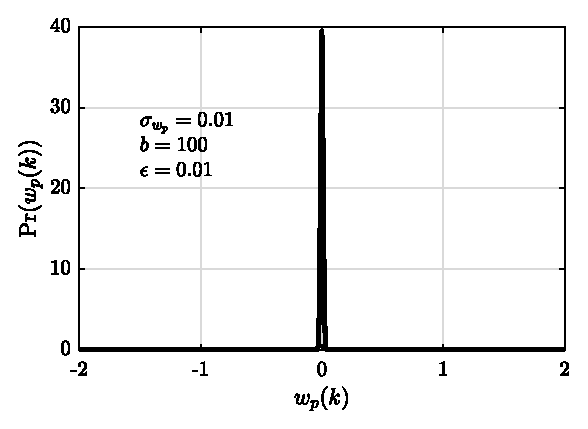
\includegraphics[width=9cm]{alpha-pdf-4.eps}
	\caption{Probability density of a random shock signal}
\end{figure}

The choice of $A(q^{-1})$ and $B(q^{-1})$ in (\ref{eq:RODD}) determines the nature of the RODD disturbance. For example, if $B(q^{-1})=1$ and $A(q^{-1})=1-q^{-1}$, $p(k)$ will be a random walk process with infrequent, large step changes, such as example (a) in Figure \ref{fig:RODDstep}.

\begin{figure}[htp] \label{fig:RODD-examples}
	%... figure contents...
\end{figure}

Denoting $\nabla=1-q^{-1}$, the \textit{RODD step-disturbance} process can be defined as

\begin{equation} \label{eq:RODD-step}
	p(k)= \frac{1}{\nabla}w_p(k)
\end{equation}

The following produces a \textit{RODD ramp-disturbance} consisting of a series of ramps with randomly-occurring changes in slope.

\begin{equation} \label{eq:RODD-ramp}
	p(k)= \frac{1}{\nabla^2}w_p(k)
\end{equation}

The following process with $0<a_1<1$ produces a RODD disturbance consisting of randomly-occurring decaying exponential changes.

\begin{equation} \label{eq:RODD-exp}
	p(k)= \frac{1}{(1-a_1q^{-1})\nabla}w_p(k)
\end{equation}

Examples of these RODD disturbances are also shown in Figure \ref{fig:RODDstep}. \textbf{TODO: Reference examples in chapter 2}

\subsection{Hidden Markov Models}

\textit{Hidden Markov models} (HMM) can be used to simulate a more diverse set of switching behaviours than those of the RODD model described in the previous section [CITE WONG \& LEE 2009]. A Markov process or Markov chain is a stochastic model used to describe a sequence of discrete events in which the probability of future events depends only on the current state [NEED A CITATION]. A HMM is a Markov model with states that are not fully observable (i.e. hidden or observed with a measurement error).

To illustrate the basic concept, we can define the state of the random shock generating process (\ref{eq:alpha2}) as a Markov model state $\gamma(k)$ with two possible values.

\begin{equation} \label{eq:gamma-k}
	\gamma(k) = 
	\begin{cases*}
		0: & no shock, \\
		1: & shock.
	\end{cases*}
\end{equation}

$\gamma(k)=0$ represents the state of the process when no shock occurs and $\gamma(k)=1$ represents the state when a shock occurs.

The switching of $\gamma(k)$ can then be defined by a Markov model \textit{transition matrix} $\Pi$ which describes the probabilities of transitioning from the state at time $k$ to the state at time $k+1$.

\begin{equation} \label{eq:Pi}
	\begin{split}
	\Pi = \left(\pi_{ij} \forall i,j\in \{1,2,...,n_j\}\right) \\
	\pi_{ij}=\Pr\left(\gamma(k)=j|\gamma(k-1)=i\right)
	\end{split}
\end{equation}

To simulate the random shock signal used in the RODD disturbance model (\ref{eq:alpha2}), the following transition probability matrix could be used.

\begin{equation} \label{eq:Pi-RODD-step}
	\Pi_{w_{p}} = \begin{bmatrix}
	1-\epsilon & \epsilon \\
	1-\epsilon & \epsilon
	\end{bmatrix}
\end{equation}

Since $w_{p}$ here is an independent random variable, it does not depend on the previous state. Therefore, the rows of the transition probability matrix are identical. 

The use of the Markov model thus allows transition probabilities which depend on the current state. For example, consider a disturbance where the signal switches infrequently between samples from two or more distributions with different parameters. The probabilities of switching from one distribution to another may be different. Such a disturbance process could be simulated with a hidden Markov model by conditioning the distribution from which $w_p(k)$ is sampled on the Markov state $\gamma(k)$.

\begin{equation} \label{eq:mog-example}
	\begin{split}
		w_p(k) \sim 
		\begin{cases*}
			\mathcal{N}\left(\mu_{w_p,1}, \sigma_{w_p,1}\right) & if $\gamma(k)=0$, \\
			\mathcal{N}\left(\mu_{w_p,2}, \sigma_{w_p,2}\right) & if $\gamma(k)=1$, \\
			... & ...\\
			\mathcal{N}\left(\mu_{w_p,n_j}, \sigma_{w_p,n_j}\right) & if $\gamma(k)=n_j-1$.
		\end{cases*} \\
	\Pr(\gamma(k)=j|\gamma(k-1)=i)=\pi_{ij} \forall i,j \in {1,2,...,n_j}
	\end{split}
\end{equation}

To make the notation more concise, let us allow the value of a time-varying discrete variable such as $A\in\left\{A_1,A_2,...,A_{n_j}\right\}$, be determined by the value of the discrete state variable $\gamma(k)$. Thus

\begin{equation} \label{eq:A-selection}
	A(\gamma(k)) = 
	\begin{cases*}
		A_1 & if $\gamma(k)=0$, \\
		A_2 & if $\gamma(k)=1$, \\
		... & ...\\
		A_{n_j} & if $\gamma(k)=n_j-1$.
	\end{cases*}
\end{equation}


With this notation, we can write (\ref{eq:mog-example}) more concisely.

\begin{equation} \label{eq:mog-example2}
	\begin{split}
		w_p(k) \sim \mathcal{N}\left(\mu_{w_p}(\gamma(k)), \sigma_{w_p}(\gamma(k))\right) \\
		\Pr(\gamma(k)=j|\gamma(k-1)=i)=\pi_{ij} \forall i,j \in {1,2,...,n_j}
	\end{split}
\end{equation}

where $\mu_{w_p}\in\left\{\mu_{w_p,1},\mu_{w_p,2},...,\mu_{w_p,n_j}\right\}$ and $\sigma_{w_p}\in\left\{\sigma_{w_p,1},\sigma_{w_p,2},...,\sigma_{w_p,n_j}\right\}$.

This model is known as a \textit{mixture of Gaussians} and can be considered a special-case of a HMM disturbance model [CITE WONG LEE].

The general HMM disturbance process can be described by the following \textit{Markov jump linear system} (MJLS) [CITE Costa 2005]. This is a state-space representation with time-varying system matrices $A(\gamma(k))$, $B(\gamma(k))$ and $C(\gamma(k))$.

\begin{equation} \label{eq:HMM}
	\begin{split}
	x_p(k+1)= A(\gamma(k))x_p(k)+B(\gamma(k))w_p(k) \\
	p(k)=C(\gamma(k))x_p(k) + e_p(k)
	\end{split}
\end{equation}

Allowing both $w_p(k)$ and $e_p(k)$ to switch as in (\ref{eq:mog-example2}), creates a very versatile stochastic model suitable for simulating a diverse family of disturbances.


\subsection{Other types of disturbances}

\begin{itemize}
	\item Discuss other possible models
	\item Describe the 
\end{itemize}



\section{State estimation}

\begin{itemize}
	\item Explain the problem of estimating RODDs using standard (e.g. Kalman) filters.
	\item Introduce multiple-model observers.
	\item Sub-optimal algorithms (Tugnait)
	\item Infrequent branching assumptions.
	\item Filter fusion - recursive Bayesian estimation for non-Gaussian processes - Generalized Pseudo-Bayesian (GPBn) methodology (Bar-Shalom and Li, 1993)
	\item Sequence pruning (adaptive) methods (AFMM).
	\item Explain how the multi-model observer concept can be used for any MJLS (time-varying A, B, C, D, Q, R matrices).
\end{itemize}

\section{System identification}

\begin{itemize}
	\item Explain Isaksson and Eriksson's perspective on standard system identification approach.
	\item Introduce other approaches—MLE, EM algorithm (Dempster et al., Wong \& Lee)
	\item Methods proposed by Bemporad (Fitting jump models, 2018 and Jump Box-Jenkins, 2020).
	\item Theory and challenges Costa book. Others?
	\item Variational Inference?
\end{itemize}

% Note: may remove this if we aren’t using any formal methods.

\section{Control strategies}

\begin{itemize}
	\item Optimal conrol—LQR, LQI for demonstration systems (linear, unconstrained).
	\item Certainty equivalence principle — E.g. using standard MPC.
	\item MPC techniques for switching systems.
\end{itemize}

\section{Grinding simulation model}

\begin{itemize}
	\item Describe model with references.
	\item Simplified flow diagram
	\item Population balance model approach - breakage and selection rates.
	\item Grate, transport delays and cyclone model.
	\item Assumptions
	\item Dynamic variables.
	\item Simulation setup - low level controls.
	\item Ore feed simulation.
	\item Figure: Particle size distributions of feed, recirculating load and product - this should help explain steady-state characteristics.
	\item Steady-state effects of ore properties on process performance - throughput, power, P80.
\end{itemize}

\section{Performance evaluation}

\begin{itemize}
	\item Tracking error of disturbance state and output estimates.
	\item Variance in steady-state.
	\item Root-mean-squared differences.
	\item Sensitivity to model errors.
	\item Closed loop stability - stability margins.
\end{itemize}

             % chapitre 1
%<articles>\include{chapitre1-articles}    % chapitre 1
%<!articles>\chapter{Methods}
\label{chap-methods}


\section{Disturbance models}

\subsection{Randomly-occurring deterministic disturbances}\label{subsec-RODD}

\textit{Randomly-occurring deterministic disturbances} (RODDs) \citep{macgregor_duality_1984} are a family of stochastic process models suitable for simulating various types of infrequently-occurring disturbances in discrete-time.  The structure of the RODD model is
\begin{equation} \label{eq:RODD}
	p(k)= \frac{B(q^{-1})}{A(q^{-1})}w_p(k),
\end{equation}
where $p(k)$ is the generated disturbance signal, $A(q^{-1})$ and $B(q^{-1})$ are arbitrary polynomial functions of the backward shift operator, $q^{-1}$, and $w_p(k)$ is a random variable generated by a switching system.

To generate randomly-occurring disturbances, the switching system,
\begin{equation} \label{eq:wpk1}
w_p(k) \sim 
\begin{cases*}
	0 & with probability $1-\epsilon$, \\
	\mathcal{N}\left(0, \sigma_{w_p}\right) & with probability $\epsilon$,
\end{cases*}
\end{equation}
may be used, where $w_p(k)$ is either 0 or is sampled from a normal distribution.  When the probability $\epsilon$ is low ($\epsilon<<1$), this system produces \textit{infrequent shocks}.

Alternatively, a mixture of two distributions may be used \citep{robertson_detection_1995}:
\begin{equation} \label{eq:wpk2}
w_p(k) \sim 
	\begin{cases*}
		\mathcal{N}\left(0, \sigma_{w_p}^2\right) & with probability $1-\epsilon$, \\
		\mathcal{N}\left(0, b^2\sigma_{w_p}^2\right) & with probability $\epsilon$.
	\end{cases*}
\end{equation}

In this formulation, $\sigma_{w_p}$ represents the standard deviation of the noise in periods between random shocks and $b$ is typically large so that the magnitude of the shocks is many times greater than $\sigma_{w_p}$. One benefit of (\ref{eq:wpk2}) is that the distribution of $w_p(k)$ is conditionally Gaussian, whereas in (\ref{eq:wpk1}) it has a non-smooth (i.e. degenerate) probability density function.

Figure \ref{fig:wpk-pdf} illustrates the probability density of $w_p(k)$ in the case of (\ref{eq:wpk2}) with $\sigma_{w_p}=0.01$, $b=100$, and $\epsilon=0.01$. Although it is difficult to discern from the plot, this is a mixture distribution with two components. The component that generates the infrequent shocks is barely visible because of its low probability. In this example, 99 percent of the probability lies within a narrow range (-0.036 < $w_p(k)$ < 0.036). However, the shocks, which occur with probability 0.01, have much higher amplitude ($b\sigma_{w_p}=1$).

\begin{figure}[htp]
	\centering
	\includegraphics[width=11.5cm]{wpk-pdf-4.pdf}
	\caption{Probability density of a random shock signal}
	\label{fig:wpk-pdf}
\end{figure}

When dealing with a system having more than one RODD, where each random shock is independent, the notation is
\begin{equation} \label{eq:wpik2}
	w_{p,i}(k) \sim 
	\begin{cases*}
		\mathcal{N}\left(0, \sigma_{w_p,i}^2\right) & with probability $1-\epsilon_i$, \\
		\mathcal{N}\left(0, b_i^2\sigma_{w_p,i}^2\right) & with probability $\epsilon_i$.
	\end{cases*},
\end{equation}
where $i \in \left\{1, 2, ..., n_p\right\}$.

The choice of $A(q^{-1})$ and $B(q^{-1})$ in (\ref{eq:RODD}) determines the nature of the RODD. For example, if $B(q^{-1})=1$ and $A(q^{-1})=1-q^{-1}$, $p(k)$ will be a random-walk process with infrequent, large step changes.

Denoting $\nabla=1-q^{-1}$, the RODD \textit{step-disturbance} process can be defined as
\begin{equation} \label{eq:RODD-step}
	p(k)= \frac{1}{\nabla}w_p(k)
\end{equation}

A RODD \textit{ramp-disturbance}, consisting of a series of ramps with randomly-occurring changes in slope, may be generated using
\begin{equation} \label{eq:RODD-ramp}
	p(k)= \frac{1}{\nabla^2}w_p(k).
\end{equation}

A RODD consisting of randomly-occurring decaying exponential changes may be generated using
\begin{equation} \label{eq:RODD-exp}
	p(k)= \frac{1}{(1-a_1q^{-1})\nabla}w_p(k),
\end{equation}
where  $0<a_1<1$.

A disturbance with a combination of different RODD types is also possible.  For example, a state-space representation of a RODD combining step changes and ramps is

\begin{equation} \label{eq:RODD-step-ramp}
	\begin{split}
		\mathbf{x}_p(k+1) & =\left[\begin{array}{cc}
			1 & 1 \\
			0 & 1
		\end{array}\right] \mathbf{x}_p(k) +\left[\begin{array}{cc}
			1 & 0 \\
			0 & 1
		\end{array}\right] \mathbf{w}_p(k) \\
		p(k) & =\left[\begin{array}{cc}
			1 & 0
		\end{array}\right] \mathbf{x}_p(k),
	\end{split}
\end{equation}

where $\mathbf{x}_p(k) \in \mathbb{R}^2$ is a state vector and $\mathbf{w}_p(k)$ is a vector of two independent random shock signals generated by (\ref{eq:wpk1}), with possibly different parameter values. Simulated examples of these RODDs are presented in figures \ref{fig:rodd-sim-plots} and \ref{fig:rodd-sim-plot2} in section \ref{chap-simulation}.

\subsection{Hidden Markov Models}

\textit{Hidden Markov models} (HMM) can be used to simulate a more diverse set of switching behaviours than those of the RODD model described in the previous section \citep{wong_realistic_2009}. A Markov process or Markov chain is a stochastic model used to describe a sequence of discrete events in which the probability of future events depends only on the current state. A HMM is a Markov model with states that are not fully observable (i.e. hidden or observed with a measurement error).

To illustrate the basic concept, we can define the state of the random shock generating process (\ref{eq:wpk2}) as a Markov model state $\gamma(k)$ with two possible values:
\begin{equation} \label{eq:gamma-k}
	\gamma(k) = 
	\begin{cases*}
		0: & no shock, \\
		1: & shock.
	\end{cases*}
\end{equation}

$\gamma(k)=0$ represents the state of the process when no shock occurs and $\gamma(k)=1$ represents the state when a shock occurs.

The switching of $\gamma(k)$ can then be defined by a \textit{transition matrix}, $\Pi$, which describes the probabilities of transitioning from the state at time $k$ to the state at time $k+1$:
\begin{equation} \label{eq:Pi}
	\begin{split}
	\Pi = \left(\pi_{ij} \forall i,j\in \{1,2,...,n_j\}\right) \\
	\pi_{ij}=\Pr\left(\gamma(k)=j|\gamma(k-1)=i\right).
	\end{split}
\end{equation}

For example, to simulate the random shock signal used in the RODD model (\ref{eq:wpk2}), the transition probability matrix
\begin{equation} \label{eq:Pi-RODD-step}
	\Pi_{w_{p}} = \begin{bmatrix}
	1-\epsilon & \epsilon \\
	1-\epsilon & \epsilon
	\end{bmatrix}
\end{equation}
is used. In this case, since $w_{p}(k)$ is an independent random variable, it does not depend on the previous state. Therefore, the rows of $\Pi_{w_{p}}$ are identical.

The use of the Markov model thus allows transition probabilities that depend on the current state. For example, consider a disturbance where the signal switches infrequently between samples from two or more distributions with different parameters. The probabilities of switching from one distribution to another may be different. Such a disturbance process could be simulated with a hidden Markov model by conditioning the distribution from which $w_p(k)$ is sampled on the Markov state $\gamma(k)$:
\begin{equation} \label{eq:mog-example}
	\begin{split}
		w_p(k) \sim 
		\begin{cases*}
			\mathcal{N}\left(\mu_{w_p,1}, \sigma_{w_p,1}\right) & if $\gamma(k)=0$, \\
			\mathcal{N}\left(\mu_{w_p,2}, \sigma_{w_p,2}\right) & if $\gamma(k)=1$, \\
			... & ...\\
			\mathcal{N}\left(\mu_{w_p,n_j}, \sigma_{w_p,n_j}\right) & if $\gamma(k)=n_j-1$.
		\end{cases*} \\
	\Pr(\gamma(k)=j|\gamma(k-1)=i)=\pi_{ij} \forall i,j \in {1,2,...,n_j}
	\end{split}
\end{equation}

To make the notation more concise, allow the value of a time-varying discrete variable such as $\sigma_{w_p} \in \left\{\sigma_{w_p,1}, \sigma_{w_p,2},..., \sigma_{w_p,n_j}\right\}$, be determined by the value of the Markov state $\gamma(k)$. Thus,
\begin{equation} \label{eq:A-selection}
	\sigma_{w_p}(\gamma(k)) = 
	\begin{cases*}
		\sigma_{w_p,1} & if $\gamma(k)=0$, \\
		\sigma_{w_p,2} & if $\gamma(k)=1$, \\
		... & ...\\
		\sigma_{w_p,n_j} & if $\gamma(k)=n_j-1$.
	\end{cases*}
\end{equation}


With this notation, (\ref{eq:mog-example}) can be written more concisely as
\begin{equation} \label{eq:mog-example2}
	\begin{split}
		w_p(k) \sim \mathcal{N}\left(\mu_{w_p}(\gamma(k)), \sigma_{w_p}(\gamma(k))\right) \\
		\Pr(\gamma(k)=j|\gamma(k-1)=i)=\pi_{ij} \forall i,j \in {1,2,...,n_j}.
	\end{split}
\end{equation}
where $\mu_{w_p}\in\left\{\mu_{w_p,1},\mu_{w_p,2},...,\mu_{w_p,n_j}\right\}$. This model is known as a \textit{mixture of Gaussians} and can be considered a special-case of a HMM-based disturbance model \citep{wong_disturbance_2007}.

The general HMM disturbance process is described by the following \textit{Markov jump linear system} (MJLS) \citep{costa_discrete-time_2005}. This is a state-space representation with time-varying system matrices $\mathbf{A}(\gamma(k))$, $\mathbf{B}(\gamma(k))$, and $\mathbf{C}(\gamma(k))$:
\begin{equation} \label{eq:HMM}
	\begin{split}
	\mathbf{x}_p(k+1) = \mathbf{A}(\gamma(k))x_p(k) + \mathbf{B}(\gamma(k))\mathbf{w}_p(k) \\
	\mathbf{p}(k) = \mathbf{C}(\gamma(k)) \mathbf{x}_p(k) + \mathbf{e}_p(k)
	\end{split}
\end{equation}

As well as $\mathbf{w}_p(k)$, $\mathbf{e}_p(k)$ may also be a switching random variable. This is a versatile dynamic model suitable for representing and simulating a diverse family of disturbances.

\subsection{Bounded disturbances}

The \textit{bounded random walk} (BRW) is a stochastic process proposed by \citep{nicolau_stationary_2002}. The discrete-time version has the difference equation

\begin{equation} \label{eq:brw}
		p(k+1) = p(k) + a(p(k)) + e(k)
\end{equation}

where $e(k)$ is a random noise with variance $\sigma_e^2$, and $a(p(k))$ is a function defined as

\begin{equation}
	a(x) = e^{\beta}\left(e^{-\alpha_{1}\left(x - \tau\right)} - e^{\alpha_{2}\left(x - \tau\right)}\right)
\end{equation}

where $\beta$, $\alpha_{1}$, and $\alpha_{2}$ are constants.  From (\ref{eq:brw}) it can be deduced that

\begin{equation}
	E(p(k+1)|p(k)) = p(k) + a(p(k)).
\end{equation}

Therefore $a(p(k))$ has the effect of an additive bias or adjustment to $p(k+1)$ which depends on $p(k)$. The shape of $a(x)$ depends on the constants. Figure \ref{fig:brw-a} shows $a(x)$ in the case where $\tau=100$, $\beta=-15$, $\alpha_{1}=3$, and $\alpha_{2}=3$.  From this, it is clear that in the vicinity of $x=\tau$, $a(x)\approx0$. When $a(p(k))=0$, (\ref{eq:brw}) is the equation for a random walk. However, outside a certain neighbourhood around $x=\tau$, $a(x)$ increases for low $x$ or decreases for high $x$. This has the effect of causing $p(k+1)$ to revert towards the mean ($\tau$) whenever $p(k)$ strays outside the neighbourhood. 

\begin{figure}[htp]
	\centering
	\includegraphics[height=5cm]{images/brw_a.pdf}
	\caption{A bounded random walk bias function}
	\label{fig:brw-a}
\end{figure}

Figure \ref{fig:brw-sim} shows a simulation of a bounded random walk with the parameter values as above, and for comparison, an unbounded random walk (labelled `RW') generated with the same noise input. The dashed lines at $p(k)=95$ and $p(k)=105$ roughly indicate the location of the lower and upper bounds which the BRW only marginally exceeds.

\begin{figure}[htp]
	\centering
	\includegraphics[height=5cm]{images/brw_sim.pdf}
	\caption{Examples of a bounded and unbounded random walk}
	\label{fig:brw-sim}
\end{figure}

Unlike a simple random walk, the BRW is stationary. \cite{nicolau_stationary_2002} derived a formula for the form of the unconditional probability distribution of the continuous-time BRW. Figure \ref{fig:brw-pdf} shows the normalized stationary probability density with the same parameter values as above. For comparison, the probability density of a random walk process after 20 sample periods is also shown. It can be seen that there is a significant probability that the random walk would exceed the bounds of this BRW after 20 sample periods. It can also be seen that the central part of the probability distribution of the BRW is flat, indicating that all values within the bounds are equally likely after a large number of samples, similar to a uniform probability distribution.

%\begin{equation}
%	p_{BRW}(x) \propto \sigma^{-2} \exp \left\{-\frac{2 e^{k}}{\sigma^{2}}\left(\frac{e^{-\alpha_{1}(x-\tau)}}{\alpha_{1}}+\frac{e^{\alpha_{2}(x-\tau)}}{\alpha_{2}}\right)\right\}
%\end{equation}

\begin{figure}[htp]
	\centering
	\includegraphics[height=5cm]{images/brw_pdf.pdf}
	\caption{Probability distributions of bounded and unbounded random walks}
	\label{fig:brw-pdf}
\end{figure}

However, the BRW as described by (\ref{eq:brw}) is not guaranteed to be stable.  For extreme values of $p(k)$, $|a(p(k))|$ may be greater than $2|p(k)|$.  This means that $|p(k)|$ will increase rapidly, leading to numerical errors in any practical implementation.  To avoid this, \cite{nicolau_stationary_2002} recommends adding a conditional regularizing step which causes reversion towards the mean, $\tau$, when the correction bias is too large. Instead of (\ref{eq:brw}), the conditional difference equation
\begin{equation} \label{eq:brw-reg}
	p(k+1) = \begin{cases*}
		p(k) + a(p(k)) + e(k) & if $\left|a(p(k)) \right| < 2\left| p(k) - \tau \right|$, \\
		\tau + \phi(p(k) - \tau) + e(k) & if $\left|a(p(k)) \right| \geq 2\left| p(k) - \tau \right|$
	\end{cases*}
\end{equation}
is used, where $\phi$ is a constant such that $0<\phi<1$. The size of $\phi$ determines how fast $p(k)$ reverts to $\tau$, the stationary mean of the BRW, when it is outside the stable region.

Since the BRW has a non-Gaussian probability distribution, analysis of the properties of any dynamical system with a BRW input is difficult. However, for simulation purposes, the BRW is a simple and practical solution to the problem of bounding a random variable.

The BRW concept can easily be extended to RODDs. For example, a RODD step disturbance (\ref{eq:RODD-step}) is a random walk with a switching noise variance (\ref{eq:wpk2}). The concern when trying to bound this disturbance is the large step change that occurs infrequently. Since the probability of the shock, as well as the sign and amplitude of the step, are independent random variables, a RODD step disturbance that happens to be at one of the bounds is as likely to step outside the bound as it is to step back inside the bounded region. Therefore, the conditional regularity used in the BRW (\ref{eq:brw-reg}) is even more important.


\section{State estimation}

State estimation is the task of estimating the values of the state variables of a dynamic model of a system given a set of measurements from the system. In process control applications, state estimates are required online (i.e. in real time), in order to provide the best possible estimate of the states at the current time (or a prediction of their values at the next time instant) in order to calculate an appropriate control action.

Consider the diagram of an input-output system model in Figure \ref{fig:model_diag_uwvy}. Here, $\mathbf{u}(k) \in \mathbb{R}^{n_u}$ is a vector of measured input variables at time instant $k$, $\mathbf{w}(k) \in \mathbb{R}^n$ is a vector of unmeasured state disturbances, $\mathbf{v}(k) \in \mathbb{R}^{n_y}$ is a vector of output disturbances or measurement errors, and $\mathbf{y}(k) \in \mathbb{R}^{n_y}$ is the vector of output variables. The box represents the mathematical model which relates the inputs to the outputs.

\begin{figure}[htp]
	\centering
	\includegraphics[width=8cm]{images/model_diag_uwvy.pdf}
	\caption{System model diagram}
	\label{fig:model_diag_uwvy}
\end{figure}

The most convenient form in which to represent discrete-time, linear, time-invariant, dynamical system models for state estimation and control purposes, is the state-space representation

\begin{equation} \label{eq:ss_rep_uwy}
	\begin{aligned}
		\mathbf{x}(k+1) = \mathbf{A} \mathbf{x}(k) + \mathbf{B} \mathbf{u}(k) + \mathbf{w}(k), \\
		\mathbf{y}(k) = \mathbf{C} \mathbf{x}(k) + \mathbf{v}(k).
	\end{aligned}
\end{equation}

where $\mathbf{x}(k) \in \mathbb{R}^n$ is a vector of state variables, $\mathbf{A} \in \mathbb{R}^{n \times n}$ is the state transition matrix, $\mathbf{B} \in \mathbb{R}^{n \times n_u}$ is the input matrix, $\mathbf{C} \in \mathbb{R}^{n_y \times n}$ is the output matrix.

\begin{figure}[htp]
	\centering
	\includegraphics[width=8cm]{images/model_diag_upwvy.pdf}
	\caption{System model with disturbance inputs and manipulatable inputs}
	\label{fig:model_diag_upwvy}
\end{figure}

The \textit{Kalman filter} \citep{kalman_new_1961} is the optimal estimator for a linear system in which the unmeasured disturbances and measurement errors are Gaussian random variables. The predictions of the states at the next time instant, $k+1$, calculated at the current time $k$, are given by
\begin{equation} \label{eq:xkp1_hat}
	\mathbf{\hat{x}}(k+1/k) = \mathbf{A} \mathbf{\hat{x}}(k/k-1) + \mathbf{B}\mathbf{u}(k) + 
	\mathbf{K}(k)\left[\mathbf{y}(k) - \mathbf{C} \mathbf{\hat{x}}(k/k-1)\right],
\end{equation}
where $\mathbf{\hat{x}}(k/k-1)$ is the previous prediction of the states at the current time, calculated in the previous time instant, $\mathbf{y}(k)$ is the current measurement of the output, and $\mathbf{K}(k) \in \mathbb{R}^{n \times n_y}$ is a correction gain matrix. An intuitive interpretation of the Kalman filter is that it iteratively updates the state estimates based on the difference between the output predicted by the system model, $\mathbf{C} \mathbf{\hat{x}}(k/k-1)$, and the output measurement ${y}(k)$.

In the case of a steady-state Kalman filter, $\mathbf{K}(k)$ is constant (time-invariant). However, in general, it is calculated at each time step using
\begin{equation} \label{eq:Kk}
	K(k) = \mathbf{A}\mathbf{P}(k/k-1)\mathbf{C}^\intercal \big(\mathbf{C}\mathbf{P}(k/k-1)\mathbf{C}^\intercal + \mathbf{R}\big)^{-1},
\end{equation}
where $\mathbf{P}(k/k-1)$ is the estimation error covariance matrix calculated in the previous time instant, and $\mathbf{R}$ is the covariance matrix of the measurement noises,
\begin{equation} \label{eq:R}
	\mathbf{R} = E\{ \mathbf{v}(k) \mathbf{v}^\intercal(k) \}.
\end{equation}

$\mathbf{P}(k/k-1)$ is updated every time step using
\begin{multline} \label{eq:Pk}
	\mathbf{P}(k+1/k) = \\ \mathbf{A}\big[\mathbf{P}(k/k-1)
	- \mathbf{P}(k/k-1)\mathbf{C}^\intercal\big(\mathbf{C}\mathbf{P}(k/k-1)\mathbf{C}^\intercal + 
	\mathbf{R}\big)^{-1}\mathbf{C}\mathbf{P}(k/k-1) \big]\mathbf{A}^\intercal + \mathbf{Q},
\end{multline}
where $\mathbf{Q}$ is the covariance matrix of estimation errors,
\begin{equation} \label{eq:Q}
	\mathbf{Q} = E\{ \mathbf{w}(k) \mathbf{w}^\intercal(k) \}.
\end{equation}

The state estimates, $\mathbf{\hat{x}}(k+1/k)$, are calculated recursively online, starting at time $k=0$, using (\ref{eq:xkp1_hat}), (\ref{eq:Kk}) and (\ref{eq:Pk}), provided that initial values of the state estimates, $\mathbf{\hat{x}}(0)$, and estimation error covariance matrix $\mathbf{P}(0)$, are available.

In the case where the system has additional disturbance inputs, $\mathbf{p}(k) \in \mathbb{R}^{n_p}$, as shown in Figure \ref{fig:model_diag_upwvy}, the state-space equations are modified to include these and the input matrix is split into two, $\mathbf{B}_u \in \mathbb{R}^{n \times n_u}$ and $\mathbf{B}_p \in \mathbb{R}^{n \times n_p}$,
\begin{equation} \label{eq:ss_rep_upwy}
	\begin{aligned}
		\mathbf{x}(k+1) = \mathbf{A} \mathbf{x}(k) + \mathbf{B}_u \mathbf{u}(k) + \mathbf{B}_p \mathbf{p}(k) + \mathbf{w}(k), \\
		\mathbf{y}(k) = \mathbf{C} \mathbf{x}(k) + \mathbf{v}(k).
	\end{aligned}
\end{equation}

For state estimation in the presence of disturbances, which is always the case in practice, a suitable model of the disturbances is needed. This additional model is shown in Figure \ref{fig:model_diag_wpupwvy} with an additional set of random variables $\mathbf{w}_p(k)$ at its input.

\begin{figure}[htp]
	\centering
	\includegraphics[width=12.5cm]{images/model_diag_wpupwvy.pdf}
	\caption{System with process model and disturbance model}
	\label{fig:model_diag_wpupwvy}
\end{figure}

A state-space representation of the combined system including the disturbance model can be constructed. This will be referred to as the \textit{augmented model},
\begin{equation} \label{eq:ss_rep_xa}
	\begin{aligned}
		\mathbf{x}_a(k+1) = \mathbf{A}_a \mathbf{x}_a(k) + \mathbf{B}_{a,u} \mathbf{u}(k) + \mathbf{B}_{a,w} \mathbf{w}_{a}(k), \\
		\mathbf{y}(k) = \mathbf{C}_a \mathbf{x}_a(k) + \mathbf{v}(k),
	\end{aligned}
\end{equation}
where $\mathbf{x}_a(k) \in \mathbb{R}^{n+n_p}$ is an augmented state vector which includes the states of both the process model and the disturbance model, and $\mathbf{w}_a(k) \in \mathbb{R}^{n+n_p}$ is an augmented vector of random variables (i.e. $\mathbf{w}(k)$ and $\mathbf{w}_p(k)$ combined).


\subsection{Multiple model approaches}

Although the random shock in a RODD is unmeasured, it may be observable from the measurements of the outputs of the system. However, as mentioned in Section \ref{chap-lit-review}, systems with RODDs pose problems for state estimation using standard Kalman filters due to the switching of the noise model parameters, namely, the variance of $w_p(k)$ (\ref{eq:wpk2}). As explained by \cite{robertson_detection_1995}, a trade-off must be made during the filter design between its ability to respond to the infrequent disturbance when it occurs, and its sensitivity to noise at other times.

Alternatively, a so-called \textit{multiple-model approach} may be considered \citep{buxbaum_recursive_1969, jaffer_estimation_1971}. Multi-model observers account for different possible hypotheses about the current and past states of the system and infer from these an overall `best' estimate of the current states. To achieve this, an independent Kalman filter is maintained for each hypothesis and a weighted average of the estimates by each filter is calculated using the conditional probabilities of each hypothesis given current and past measurements.

Let the number of Kalman filters be $n_f$ and the \textit{shock occurrence hypothesis} associated with Kalman filter $f$ at time instant $k$ be
\begin{equation} \label{eq:gammak}
	\gamma_{f}(k) \in \left\{0, 1 \right\} \forall{k \ge 0}.
\end{equation}

First, consider the case of estimating only one shock signal (\ref{eq:wpk2}). Therefore, $\gamma_{f}(k)$ is a scalar. The transition probabilities of the random shock are independent of previous shocks:
\begin{equation} \label{eq:Pr_gammak_given_gammakm1}
	\begin{aligned}
		& \Pr\left(\gamma_{f}(k)=0 \mid \gamma_{f}(k-1)\right) = 1-\epsilon, \\
		& \Pr\left(\gamma_{f}(k)=1 \mid \gamma_{f}(k-1)\right) = \epsilon.
	\end{aligned}
\end{equation}

After $k$ time steps, the complete shock occurrence hypothesis associated with filter $f$ is
\begin{equation} \label{eq:Gammak}
	\Gamma_f(k) = \left\{\gamma_f(0), \gamma_f(1), ..., \gamma_f(k) \right\}.
\end{equation}

The measurements up to time $k$ are
\begin{equation} \label{eq:Uk_Yk}
	\begin{aligned}
		\mathbf{U}(k)=\left\{\mathbf{u}(0), \mathbf{u}(1), ..., \mathbf{u}(k) \right\} \\
		\mathbf{Y}(k)=\left\{\mathbf{y}(0), \mathbf{y}(1), ..., \mathbf{y}(k) \right\}.
	\end{aligned}
\end{equation}

Assume that new measurement data is made available at each time instant. The probability of the shock sequence associated with filter $f$ given the data up to time $k-1$ can be calculated recursively:
\begin{multline} \label{eq:Pr_Gammakp1_given_Yk}
	\Pr(\Gamma_f(k) \mid \mathbf{Y}(k-1)) = 
	\Pr(\gamma_f(k) \mid \gamma_f(k-1)) \Pr(\Gamma_f(k-1) \mid \mathbf{Y}(k-1)).
\end{multline}
The conditional probability densities of the measurements $\mathbf{y}(k)$ are approximated by Gaussian distributions
\begin{equation} \label{eq:p_yk_given_Gammak_Ykm1}
	p(\mathbf{y(k)} \mid \Gamma_f(k), \mathbf{Y}(k-1)) \approx
	\mathcal{N}\left(\mathbf{y}(k), \mathbf{C} \mathbf{\hat{x}}_{f}(k/k-1), \mathbf{C} \mathbf{P}_f(k/k-1) \mathbf{C}^\intercal+\mathbf{R}\right)
\end{equation}
where $p(\cdot)$ here represents a probability density function, $\mathbf{\hat{x}}_{f}(k/k-1)$ and $\mathbf{P}_f(k/k-1)$ are the state estimates and estimate covariances of each Kalman filter at the previous time step, and $\mathcal{N}(\mathbf{y}, \mathbf{\mu}, \Sigma)$ is the multivariate normal probability density of $\mathbf{y}$ with mean $\mathbf{\mu}$ and variance $\Sigma$.

The estimate of the probability of the shock sequence $\Gamma_f(k)$ given the data up to time $k$ is
\begin{equation} \label{eq:Pr_Gammak_given_Yk}
	\Pr(\Gamma_f(k) \mid \mathbf{Y}(k)) = \frac{q_f(k)}{\sum_{f=1}^{n_f} q_f(k)},
\end{equation}
where
\begin{equation} \label{eq:qfk}
	q_f(k) = p(\mathbf{y}(k) \mid \Gamma_f(k), \mathbf{Y}(k-1)) \Pr(\Gamma_f(k) \mid \mathbf{Y}(k-1)).
\end{equation}

The Kalman filters for tracking each hypothesis use the state-space representation of the augmented system model (\ref{eq:ss_rep_xa}). 
However, in the case of a system with a RODD, the disturbance inputs include the non-Gaussian random variable, $\mathbf{w}_p(k)$, as well as the usual Gaussian disturbances on the rest of the states, $\mathbf{w}(k)$:
\begin{equation} \label{eq:wak}
	\mathbf{w}_a(k) = \begin{bmatrix}
		\mathbf{w}(k) \\
		\mathbf{w}_p(k)
	\end{bmatrix}.
\end{equation}

The system is therefore a \textit{hybrid dynamical system} because it has a switching noise covariance matrix. Define the set of possible covariance matrices as
\begin{equation} \label{eq:init_Q_R}
	\mathcal{Q} = \left\{\mathbf{Q}_0, \mathbf{Q}_1\right\},
\end{equation}

and, for convenient notation, let $\mathcal{Q}$ be indexed by the shock indicator variable $\gamma_f(k)$:
\begin{equation} \label{eq:init_Q}
	\mathcal{Q}(\gamma_f(k)) = 
	\begin{cases*}
		\mathbf{Q}_0 & \text{if} $\gamma_f(k)=0$, \\
		\mathbf{Q}_1 & \text{if} $\gamma_f(k)=1$.
	\end{cases*}
\end{equation}

At the start of simulation, filter $f$ has an initial estimate of the states, $\mathbf{\hat{x}}_f(0)$, and an initial estimate covariance $\mathbf{P}_f(0)$. At each time instant, starting at $k=0$, the filter correction gain is updated as in (\ref{eq:Kk})
\begin{equation} \label{eq:Kf}
	K_f(k) = \mathbf{A}\mathbf{P}_f(k/k-1)\mathbf{C}^\intercal \big(\mathbf{C}\mathbf{P}_f(k/k-1)\mathbf{C}^\intercal + \mathbf{R}\big)^{-1},
\end{equation}

the corrected state estimate at time $k+1$ is calculated as in \ref{eq:xkp1_hat}
\begin{equation} \label{eq:xfkp1_hat}
	\mathbf{\hat{x}}_f(k+1/k) = \mathbf{A} \mathbf{\hat{x}}_f(k/k-1) + \mathbf{B}\mathbf{u}(k) + 
	\mathbf{K}_f(k)\left[\mathbf{y}(k)-\mathbf{C} \mathbf{\hat{x}}_f(k/k-1)\right],
\end{equation}

and the estimation error covariance is updated using
\begin{multline} \label{eq:Pfk}
	\mathbf{P}_f(k+1/k) = \mathbf{A}\big[\mathbf{P}_f(k/k-1)
	- \mathbf{P}_f(k/k-1)\mathbf{C}^\intercal\big(\mathbf{C}\mathbf{P}_f(k/k-1)\mathbf{C}^\intercal \\ + 
	\mathbf{R}\big)^{-1}\mathbf{C}\mathbf{P}_f(k/k-1) \big]\mathbf{A}^\intercal + \mathcal{Q}(\gamma_f(k)). \\
\end{multline}

Note the difference between (\ref{eq:Pfk}) and (\ref{eq:Pk}).  Here, $\mathbf{P}_f(k+1/k)$ is dependent on $\gamma_f(k)$, which determines the noise covariance matrix used in the update, whereas in (\ref{eq:Pk}), $\mathbf{Q}$ is time invariant.

Finally, the multi-model observer estimate of the states in the next time instant is the sum of the $n_f$ Kalman filter estimates weighted by their conditional probabilities:
\begin{equation} \label{eq:x_hat}
	\mathbf{\hat{x}}(k+1/k) = \sum_{f=1}^{n_f} \mathbf{\hat{x}}_f(k+1/k) \Pr(\Gamma_f(k) \mid \mathbf{Y}(k))
\end{equation}

% TODO: in Robertson et al, they estimate x(k/k) not x(k+1/k).

Algorithm \ref{alg:afmm} is the iterative algorithm used to execute these computations.

\begin{algorithm}
	\caption{Multiple model observer calculations}  \label{alg:afmm}
	%\algorithmfootnote{$y_0$ denotes the initial value.}
	\begin{algorithmic}
			\Require $\mathbf{A},\mathbf{B},\mathbf{C},\mathbf{\hat{x}}(0), \mathbf{P}(0), \mathcal{Q}, \mathbf{R}, \epsilon, \mathbf{U}(N), \mathbf{Y}(N)$
			\State $\mathbf{\hat{x}}_1(0) \gets \mathbf{\hat{x}}(0)$  \Comment{Initialize Kalman filters}  % \footnotemark
			\State $\mathbf{P}_1(0) \gets \mathbf{P}(0)$
			\State $\Pr(\Gamma_1(k-1)|\mathbf{Y}(k-1))) \gets 1$
			\For{$f \gets 2, n_f$}
			\State $\mathbf{\hat{x}}_f(0) \gets \mathbf{\hat{x}}(0)$
			\State $\mathbf{P}_f(0) \gets 10^{10}\mathbf{P}(0)$
			\State $\Pr(\Gamma_f(k-1)|\mathbf{Y}(k-1))) \gets 1^{-10}$
			\EndFor
			\For{$k \gets 0, N$}
			\State $\Gamma_f(k), \mathbf{\hat{x}}_f(k), \mathbf{P}_f(k) \gets ...$ \Comment{Sub-optimal procedure occurs here}  % \footnotemark
			\For{$f \gets 1, n_f$}
			\State calculate $\Pr(\Gamma_f(k) \mid \mathbf{Y}(k))$ (\ref{eq:Pr_Gammakp1_given_Yk}, \ref{eq:p_yk_given_Gammak_Ykm1}, \ref{eq:Pr_Gammak_given_Yk}, \ref{eq:qfk})
			\State calculate $\mathbf{K}_f(k)$ (\ref{eq:Kf}) \Comment{Filter updates}
			\State calculate $\mathbf{\hat{x}}_f(k+1/k)$ (\ref{eq:xfkp1_hat})
			\State update $\mathbf{P}_f(k+1/k)$ (\ref{eq:Pfk})
			\EndFor
			\State calculate $\mathbf{\hat{x}}(k+1/k)$ (\ref{eq:x_hat}) \Comment{State estimate}
			\State calculate $\mathbf{P}(k+1/k)$ \Comment{Error covariance}  % \footnotemark
			\EndFor
		\end{algorithmic}
\end{algorithm}

% Version with footnotes - not working
%\begin{algorithm}
%	\caption{Multiple model observer calculations} \label{alg:afmm}
%	%\algorithmfootnote{$y_0$ denotes the initial value.}
%	\begin{algorithmic}
%		\Require $\mathbf{A},\mathbf{B},\mathbf{C},\mathbf{\hat{x}}(0), \mathbf{P}(0), \mathcal{Q}, \mathbf{R}, \epsilon, \mathbf{U}(N), \mathbf{Y}(N)$
%		\State $\mathbf{\hat{x}}_1(0) \gets \mathbf{\hat{x}}(0)$  \Comment{Initialize Kalman filters\footnotemark}
%		\State $\mathbf{P}_1(0) \gets \mathbf{P}(0)$
%		\State $\Pr(\Gamma_1(k-1)|\mathbf{Y}(k-1))) \gets 1$
%		\For{$f \gets 2, n_f$}
%		\State $\mathbf{\hat{x}}_f(0) \gets \mathbf{\hat{x}}(0)$
%		\State $\mathbf{P}_f(0) \gets 10^{10}\mathbf{P}(0)$
%		\State $\Pr(\Gamma_f(k-1)|\mathbf{Y}(k-1))) \gets 1^{-10}$
%		\EndFor
%		\For{$k \gets 0, N$}
%		\State $\Gamma_f(k), \mathbf{\hat{x}}_f(k), \mathbf{P}_f(k) \gets ...$ \Comment{Sub-optimal procedure occurs here\footnotemark}
%		\For{$f \gets 1, n_f$}
%		\State calculate $\Pr(\Gamma_f(k) \mid \mathbf{Y}(k))$ (\ref{eq:Pr_Gammakp1_given_Yk}, \ref{eq:p_yk_given_Gammak_Ykm1}, \ref{eq:Pr_Gammak_given_Yk}, \ref{eq:qfk})
%		\State calculate $\mathbf{K}_f(k)$ (\ref{eq:Kf}) \Comment{Filter updates}
%		\State calculate $\mathbf{\hat{x}}_f(k+1/k)$ (\ref{eq:xfkp1_hat})
%		\State update $\mathbf{P}_f(k+1/k)$ (\ref{eq:Pfk})
%		\EndFor
%		\State calculate $\mathbf{\hat{x}}(k+1/k)$ (\ref{eq:x_hat}) \Comment{State estimate}
%		\State calculate $\mathbf{P}(k+1/k)$ \Comment{Error covariance\footnotemark}
%		\EndFor
%	\end{algorithmic}
%\end{algorithm}
%
%\addtocounter{footnote}{-3} %3=n
%\stepcounter{footnote}\footnotetext{To initialize the bank of $n_f$ Kalman filters, initialize one with an available estimate and covariance of the initial state of the system and set the covariances of all others to high values to ensure they are eliminated as soon as better estimates are available.}
%\stepcounter{footnote}\footnotetext{At this point, the algorithm must extend the shock indicator sequences to the current time instant, while limiting the total number of hypotheses and filters according to a particular sub-optimal method such as the procedures described in section \ref{subsec-pruning} and \ref{subsec-fusion}.
%\stepcounter{footnote}\footnotetext{The estimation error covariance is not required by the algorithm. It may be calculated if needed.}

\subsection{Sub-optimal algorithms}

\begin{itemize}
	\item Sub-optimal algorithms (Tugnait)
	\item Approximation 1: Infrequently-occurring disturbances -> infrequent branching assumptions.
	\item Approximation 2: Infrequently-occurring disturbances -> less combinations of disturbances.
	\item Approximation 3: Filter fusion - 
	\item Recursive Bayesian estimation for non-Gaussian processes
	\item Generalized Pseudo-Bayesian (GPBn) methodology (Bar-Shalom and Li, 1993).
	\item Alternative sub-optimal approach: Sequence pruning (adaptive) methods 
	\item Describe branching and pruning procedure of AFMM.
	\item Explain how the multi-model observer concept can be used for any MJLS (time-varying A, B, C, D, Q, R matrices).
\end{itemize}

The problem that sub-optimal algorithms address is the inevitable increase in the number of hypotheses that must be modelled in an optimal multi-model observer. For a system with one RODD disturbance, the number of possible hypotheses doubles at each time step because each current hypothesis branches into two—one corresponding to the assumption of no shock in the next time period and the other to that of a shock. Figure \ref{fig:mm-obs-br} illustrates that after 3 time instants starting at $k=0$, eight hypotheses are needed to represent the possible shock sequences. For a system with two independent RODD disturbances, the number would be 64.

\begin{figure}[htp]
	\centering
	\includegraphics[height=7.5cm]{images/mm_obs_seq_br.pdf}
	\caption{Sequence branching}
	\label{fig:mm-obs-br}
\end{figure}


\subsubsection{Sequence fusion} \label{subsec-fusion}

\cite{robertson_detection_1995} propose a sub-optimal approach for RODD state estimation combining three approximations. The first is referred to as \textit{sequence fusion} or the \textit{generalized pseudo-Bayes algorithm} \citep{buxbaum_recursive_1969, jaffer_estimation_1971, tugnait_detection_1982}. This is based on the assumption that only recent differences in the shock hypothesis sequences are important for state estimation. Therefore, sequences which have the same values over the previous $f$ sample times, $\{\gamma(k-f+1), ...,  \gamma(k-1), \gamma(k)\}$, are combined. In other words, the maximum length of the unique sequences that must be modelled is $f$, which is known as the \textit{fusion horizon}. \textbf{TODO: $f$ clashes with use of $f$ as a filter index variable}

Secondly, they assume that the exact timing of the random shocks is not important and define \textit{detection intervals} of more than one sample period during which it is assumed that only one shock may occur. This is based on the observation that when the correction gain of a Kalman filter is increased, it tends to remain large for several sample periods. The probability of at least one random shock during a detection interval of length $d$ sample times is therefore
\begin{equation} \label{eq:p_gamma_d}
	\epsilon_d = 1 - (1 - \epsilon)^d.
\end{equation}

The probabilities of the modelled random shocks are then redefined as
\begin{equation} \label{eq:Pr_gamma_nd}
	\begin{aligned}
		\Pr\left(\gamma_{f}(k)=0\right) = \begin{cases*}
			1 - \epsilon_d & \text { for } $k = d, 2d, \ldots$ \\
			1 & \text { for } $k \ne d, 2d, \ldots$
		\end{cases*} \\
		\Pr\left(\gamma_{f}(k)=1\right) = \begin{cases*}
			\epsilon_d & \text { for } $k = d, 2d, \ldots$ \\
			0 & \text { for } $k \ne d, 2d, \ldots$
		\end{cases*} \\
	\end{aligned}
\end{equation}

Thirdly, they rely on the fact that the random shocks occur infrequently and therefore the probability that more than $m$ shocks occur during the fusion horizon is low, where $m$ may be 1 or a low number. This further reduces the number of filters required.

To illustrate this sequence fusion procedure, consider a simple example. Suppose there is one RODD to estimate and a sequence fusion algorithm is used with a detection interval of $d=3$ and a maximum number of shocks over the fusion horizon of $m=1$. Figure \ref{fig:mm-obs-seq-rob1} shows the four hypotheses that would be required in this case. Note that hypothesis 1 assumes no shocks at any time. Hypothesis 2 assumes shocks occur at times $k=0,9,18,...$. Hypothesis 3 assumes shocks occur at times $k=3,12,21,...$, and so on. After $f=9$ sample periods the sequences repeat indefinitely. 
\begin{figure}[htp]
	\centering
	\includegraphics[height=5.3cm]{images/mm_obs_seq_rob1.pdf}
	\caption{Sequence fusion example 1 ($d=3$, $m=1$, $f=9$)}
	\label{fig:mm-obs-seq-rob1}
\end{figure}
If a shock actually occurred in the system at time $k=4$, for example, then the algorithm should estimate that hypothesis 3 is the most likely because this assumes a shock occurred at $k=3$, which is the close to reality.

Figure \ref{fig:mm-obs-seq-rob2} illustrates a second example of the sequence fusion algorithm with $m=2$ and a longer detection interval, $d=5$.  Note that this also has four hypotheses and that hypothesis 4 includes the case of two shocks within the fusion horizon. As in the previous example, if a true shock occurred at time $k=4$, the estimated most likely hypothesis should be hypothesis 3 because it assumes one shock occured at $k=5$, which is close to reality.

\begin{figure}[htp]
	\centering
	\includegraphics[height=5.3cm]{images/mm_obs_seq_rob2.pdf}
	\caption{Sequence fusion example 2 ($d=5$, $m=2$, $f=10$)}
	\label{fig:mm-obs-seq-rob2}
\end{figure}

\cite{robertson_detection_1995} describe a systematic procedure to choose the $f$, $d$, and $m$ parameters, and give the formula for the total probability of the modelled hypotheses up to time $k=nd$:
\begin{equation} \label{eq:p_gamma}
	\operatorname{Pr}\left(\sum_{i=1}^{n} \gamma(i d) \leq m\right) = \sum_{j=0}^{m} \binom{n}{j} \epsilon_p^{n-j}(1-\epsilon_p)^{j},
\end{equation}
where $\binom{n}{j}$ represents the number of possible combinations of $j$ shocks in $n$ intervals. They recommend that the total probability modelled should be at least 0.99 to ensure that only low-probability hypotheses are ignored.

In a later paper, \cite{robertson_method_1998} describe a variation to the sequence fusion algorithm described above.  Rather than assuming that the shock occurs in the first sample period of each detection interval, as shown in Figures \ref{fig:mm-obs-seq-rob1} and \ref{fig:mm-obs-seq-rob2}, they propose to represent the shock as a sequence of $d$ smaller shocks such that the total variance over the detection interval is the same as that of one shock. They claim that this improved the performance of the algorithm in simulations.

To implement this, first define a new variable to represent whether or not at least one shock occurs during the $n$\textsuperscript{th} detection interval:

\begin{equation} \label{eq:deltak}
	\delta(n) = \begin{cases*}
		0 & \text{if} $\sum_{k=(n-1) d}^{n d-1} \gamma_{k}=0$, \\
		1 & \text{if} $\sum_{k=(n-1) d}^{n d-1} \gamma_{k}\ge0$.
	\end{cases*}
\end{equation}

Then, replace the random shock variable used at each sample time, $w_p(k)$ (\ref{eq:wpk2}), with:
\begin{equation} \label{eq:wpdk}
	w_{p,d}(k) \sim 
	\begin{cases*}
		\mathcal{N}\left(0, \sigma_{w_p}^2\right) & \text{when} $\delta(n) = 0$, \\
		\mathcal{N}\left(0, \frac{b^2\sigma_{w_p}^2}{d}\right) & \text{when} $\delta(n) = 1$.
	\end{cases*}
\end{equation}

Note that the variance of a single shock, $b^2\sigma_{w_p}^2$, is divided by the interval length $d$.

\subsubsection{Sequence pruning} \label{subsec-pruning}

\textit{Sequence pruning} is the selective branching and deletion of shock hypotheses that have a low likelihood given the current measurements. The \textit{adaptive forgetting through multiple models} (AFMM) algorithm by \cite{andersson_adaptive_1985}, which was used by \cite{eriksson_classification_1996} for RODD estimation, uses sequence pruning to limit the number of filters required. In this algorithm, the current set of hypotheses are ranked at each time step, according to their conditional probabilities calculated using (\ref{eq:Pr_Gammak_given_Yk}). The hypothesis with the lowest probability is then pruned with the caveat explained below. The most probable hypothesis is allowed to branch but all other hypotheses are advanced assuming no shock occurs in the next time period (i.e. all but one of their branches are pruned). This makes sense in the case of RODD disturbances because the probability of a shock is low. Thus, the total number of hypotheses and filters is capped at a fixed number, $n_f$.

The caveat mentioned above, is that no hypothesis may be eliminated less than $n_{min}$ time steps after being created. This is to prevent good hypotheses from being eliminated before the conditional probabilities have been properly estimated, which can take more than one sample period. For this reason, $n_f$ must be at least sufficient to accommodate the \textit{minimum life}, $n_{min}$, of new hypotheses. Note that in the case of systems with more than one RODD disturbance, the number of branches of the most likely sequence is more than two, therefore a larger number of sequences will be pruned at each sample time.

To illustrate the sequence pruning procedure, consider the diagram in Figure \ref{fig:mm-obs-seq-erik}. This shows the possible evolution of the hypothesis sequences in response to an actual shock sequence consisting of one shock at time $k=4$.  The most likely hypotheses at each time instant, identified by the circles with thicker outlines, branch into two at the next time instant. After the limit of five hypotheses is reached, one hypothesis is pruned at each sample time and replaced by a new branched hypothesis at the next sample time. At time $k=6$, hypothesis 2 becomes the most likely based on the available measurements at that time. Also note that no new branches are terminated in less than two sample times.

\begin{figure}[htp]
	\centering
	\includegraphics[height=7.5cm]{images/mm_obs_seq_erik.pdf}
	\caption{Sequence pruning example ($n_f=5$, $n_{min}=2$)}
	\label{fig:mm-obs-seq-erik}
\end{figure}

The AFMM algorithm by \cite{gustafsson_estimation_1993} includes a procedure for online estimation of the measurement noise covariance using a forgetting factor to control the speed of adaptation of the estimates. This component was not implemented in this work since it is assumed the measurement noise is time invariant.

\section{System identification}

Outline notes:
\begin{itemize}
	\item Explain Isaksson and Eriksson's perspective on standard system identification approach.
	\item Explain distinction between system detection or 'discrimination' and system identification, reference Isaksson and Eriksson's paper on disturbance classification (whether disturbance at input or output of process).
	\item Introduce other approaches—MLE, EM algorithm (Dempster et al., Wong \& Lee)
	\item Methods proposed by Bemporad (Fitting jump models, 2018 and Jump Box-Jenkins, 2020).
	\item Theory and challenges Costa book. Others?
	\item In recent years, numerical methods to overcome the intractability of the probabilistic integral have received a lot of attention.
	\item Sequential Monte-Carlo methods, (incl. particle filtering), Stochastic Variational Inference, ... (read Special issue in IEEE control magazine for an overview of these methods)
\end{itemize}

% Note: may remove this if we aren’t using any formal methods.

\section{Control strategies}

In this work, the goal is to test the performance of different observers in a closed-loop feedback control application (not to evaluate different control strategies). Therefore, only one control strategy is considered. According to the \textit{separation principle} of estimation and control, the control strategy may be designed independently of the observer. The controller is designed using the same model of the augmented system, including the plant model and disturbance models. However, the switching behaviour of the random shock variable used in the RODD is not explicitly considered in the control design. The estimates of the model states produced by the observer are assumed to be optimal, i.e. the expected values, and their uncertainty is not taken into account by the control algorithm or in its design.


\subsection{Model predictive control}

\textit{Model predictive control} (MPC) is a well known and widely used multi-variable control algorithm used in industrial applications. This is largely due to the fact that constraints can be imposed on the manipulatable variables and control variables, as well as its intuitive design and the ease with which it can be tuned to achieve control objectives \citep{maciejowski_predictive_2002}. Although it is a computationally complex algorithm, numerous proven commercial products exist to enable its implementation.

MPC utilizes a prediction equation based on the dynamic model of the system to find feasible future trajectories of the system outputs as a function of the manipulatable variables and the states of the model at the current. The length of the prediction horizon, $H_p$, is defined in terms of the number sample times starting at the next time instant, $k+1$. The predicted outputs over the prediction horizon, calculated at the current time $k$, are denoted $\hat{\textbf{y}}(k+i / k)$ for $i=1,2,...,H_p$. The length of the control horizon, $H_c$, is defined starting at the current time, $k$, and the manipulatable inputs are denoted $\mathbf{u}(k+i-1)$ for $i=1,2,...,H_c$. The control horizon is usually shorter than the prediction horizon, in which case, $\mathbf{u}(k+j)=\mathbf{u}(k+H_c-1)$ for $j=H_c,H_c+1,...,H_p$.

The constrained optimization problem, which is solved at each time step, is
\begin{align} \label{eq:mpc-opt}
	\begin{split}
		\min _{\mathbf{u}(k), \mathbf{u}(k+1), \ldots, \mathbf{u} (k+H_c-1)}
		& \quad \sum_{i=1}^{H_{p}}[\mathbf{\hat{y}}(k+i / k) - \mathbf{r}(k+i)]^\intercal \mathbf{\Phi} [\mathbf{\hat{y}}(k+i / k) - \mathbf{r}(k+i)] \\
		& \qquad + \sum_{i=1}^{H_{c}}[\Delta \mathbf{u}(k+i-1)]^\intercal \mathbf{\Lambda} [\Delta \mathbf{u}(k+i-1)] \\
			\end{split} \\
		\text { subject to: }
		&\ \mathbf{u}_{min} \leq \mathbf{u}(k+j-1) \leq \mathbf{u}_{max} \quad  j=1,2, \dots, H_{c} \label{eq:mpc-cons-1}, \\
		& \Delta \mathbf{u}_{min} \leq \Delta \mathbf{u}(k+j-1) \leq \Delta \mathbf{u}_{max} \quad j=1,2, \dots, H_{c}, \label{eq:mpc-cons-2} \\
		& \mathbf{y}_{min} \leq \mathbf{\hat{y}}(k+j / k) \leq \mathbf{y}_{max} \quad  j=1,2, \dots, H_{p}, \label{eq:mpc-cons-3}
\end{align}
where $\mathbf{r}(k+i)$ for $i=1,2,...,H_p$ is the reference output trajectory, and $\Delta \mathbf{u}(k)$ is the change in the manipulatable variable at time $k$, defined as $\Delta \mathbf{u}(k) = \mathbf{u}(k) - \mathbf{u}(k-1)$. The tunable parameters are $H_p$, $H_c$, $\mathbf{\Phi}$, and $\mathbf{\Lambda}$, and the constraints are $\mathbf{u}_{min}$, $\mathbf{u}_{max}$, $\Delta \mathbf{u}_{min}$, $\Delta \mathbf{u}_{max}$, $\mathbf{y}_{min}$, and $\mathbf{y}_{max}$. Note that the last constraint (\ref{eq:mpc-cons-3}) only guarantees that the estimate of the system output will not violate the constraints. This does not imply that the true system output will respect them at all times.

Once a solution to the optimization problem is found, only the control actions at the current time, $\mathbf{u}(k)$, are transmitted to the plant. The procedure is then repeated every future time instant to compute the subsequent control actions. This is referred to as a \textit{receding horizon control}.


\section{Grinding simulation model}

Outline notes:
\begin{outline}
    \1 Assumptions and limitations: constant breakage rate model, relationships between speed, media, trajectories, filling level and breakage not captured.
	\1 Describe grate, transport delays and cyclone model.
	\1 Outline any significant changes made from Edgar's model
	\1 Figure: simulation results showing steady-state characteristics - e.g. power, grind, and throughput vs. fill level and speed.
	\1 Figure \ref{fig:coarse_fine_psd_plot}: Particle size distributions of feed, recirculating load and product - this should help explain steady-state characteristics.
	\1 Figure - Step responses of main process variables to changes in ore properties.
	\1 Selection of particle size distribution as the disturbance variable for this work.
	\1 Steady-state characteristics with operating points (grind curves)\\
\end{outline}


A dynamic simulation model of the primary grinding circuit of a gold mine in Quebec is used to simulate the effects of changes in ore feed properties over time. The model was developed by \cite{perez_garcia_dynamic_2020} following the methodology described by \cite{grimble_dynamic_2010} and was calibrated to match the operating data from the real plant \citep{perez-garcia_systematic_2020}. The SAG mill component is a \textit{population balance model} with 24 discrete size intervals for ore particles with constant specific-energy selection rates (i.e. breakage rates are proportional to total energy consumption) and a constant breakage matrix.

Figure \ref{fig:sag-diag} is a simplified diagram of the simulated circuit, consisting of a feed conveyor, SAG mill, pump box, pump, and a bank of hydro-cyclones.
\begin{figure}[htp]
	\centering
	\includegraphics[width=11cm]{images/sag-circuit-diag.pdf}
	\caption{Simplified process flow diagram}
	\label{fig:sag-diag}
\end{figure}
For the purposes of this work, two ore streams with different PSDs were configured to feed the circuit. Each stream is a different mix of two different ores. One ore has a fine PSD and the other is coarse. The mix for stream \#1 (`mix 1') consists of 22.83\% coarse ore (\textit{mix factor} of 0.2283) and mix \#2 is an even mix of both ores (mix factor of 0.5). Figure \ref{fig:coarse_fine_psd_plot} shows the PSDs of the two ore sources and the two mixtures.

\begin{figure}[htp]
	\centering
	\includegraphics[width=9cm]{images/coarse_fine_psd_plot.pdf}
	\caption{Ore particle size distributions}
	\label{fig:coarse_fine_psd_plot}
\end{figure}

The SAG mill water addition set-point is set by ratio control to a ratio of the fresh ore feed rate. This ratio may be manipulated by the control system. The pump-box level has a PI (proportional-integral) controller to control the level to a fixed set-point by manipulating the water addition rate set-point. The discharge pump speed is fixed. Conveyor speed is adjusted automatically in response to the fresh ore feed rate. Total ore feed rate and the SAG rotational speed set-point may also be manipulated by a control system.

The main measurable process variables are mill weight, power consumption, circulating load flow rate, and the solids-content (\%) of the cyclone feed. The P80 (80\% passing size) of the ground product leaving the cyclone overflow is also measured. Mill filling level and many other simulation variables are available for analysis but are assumed to be unmeasured in the real operation and therefore not available for process control.

Zero-mean Gaussian measurement noises are added to the output variables to simulate measurement errors. The parameters for these noises and other information on all the process variables are shown in Table X. Except for the measurement noises and the input disturbances described in subsequent sections, the model itself is deterministic.

%TODO: Table of process variables and normal operating points, limits etc.

Although some of these process variables would likely be sampled at higher rates in practice, it is assumed, for simplicity, that they are all sampled at the same rate of 1 sample every 3 minutes (i.e. a sampling period of 0.05 hours). This was deemed to be a typical sampling rate of a standard online particle size analyser that would be used for the P80 measurement.


\section{Performance evaluation}

Outline notes:
\begin{itemize}
	\item Comparing disturbance state estimate to true disturbance (simulation only).
	\item Tracking error: Mean-squared difference of output estimates. (or use RMSE?)
	\item Partitioning of simulation outputs into 'transition periods' and steady-state periods.
	\item Variance of output estimate in steady-state (no disturbances).
	\item Mean-squared differences in estimates (similar to variance but with no bias).
	\item Sensitivity to model errors, observer parameters.
	\item Closed loop stability - stability margins.
\end{itemize}

             % chapitre 2, etc.
%<articles>\chapter{<Titre du chapitre ou de l'article>}     % numéroté
\label{chap-}                   % étiquette pour renvois (à compléter!)

\section{Résumé}

\begin{otherlanguage*}{french}
  <Résumé de l'article en français. Obligatoire.>
\end{otherlanguage*}

\section{Abstract}

\begin{otherlanguage*}{english}
  <English abstract of the paper. Optional, but recommended.>
\end{otherlanguage*}

<Texte du chapitre ou de l'article.>

\bibliographystyle{}              % style de la bibliographie
\bibliography{}                   % production de la bibliographie
    % chapitre 2, etc.
% !TEX encoding = UTF-8 Unicode
\chapter*{Conclusion}           % ne pas numéroter
\label{chap-conclusion}         % étiquette pour renvois
\phantomsection\addcontentsline{toc}{chapter}{\nameref{chap-conclusion}} % inclure dans TdM

\textbf{NOT COMPLETE}

\begin{itemize}
	\item Summarize results
	\item Summarize issues/drawbacks and potential ways to mitigate them.
	\item Identify gaps and suggest areas of further research/data collection.
	\item Reiterate potential benefits and need to quantify these.
\end{itemize}

% Text from IFAC paper
While the multi-model observer has a number of clear advantages over a single Kalman filter, its limitations are important to recognize. Firstly, the higher variance of the noise model during the transitions, which is needed for a fast response, also increases the variance of the estimates during these periods, resulting in larger errors---46\% higher than those of KF3 during transition periods.

Secondly, the multiple-model algorithm is limited to infrequently-occurring disturbances where the disturbance model is known. Finally, the complexity of the algorithm is a significant disadvantage from the perspective of practical implementation.




            % conclusion

\appendix                       % annexes le cas échéant

\chapter{Additional results and sensitivity analysis}     % numérotée
\label{chap-Annex}                   % étiquette pour renvois (à compléter!)

\section{Multiple model observer algorithms}

\begin{itemize}
	\item Multi-model algorithm.
\end{itemize}

\section{Tuning of sequence fusion algorithm 1995 variant}

The sequence fusion algorithm evaluated in section \ref{section:sim-obs-lin} is based on \cite{robertson_method_1998}. However, Robertson and coworkers published results in 1995 \citep{robertson_detection_1995} using a slightly different version of this algorithm. Table \ref{tb:obs-sim1-popt-SF95} shows the results of a parameter search for the earlier version of the algorithm using the same simulation data used to tune the 1998 algorithm.

\begin{table}[hb]
	\begin{center}
		\caption{Multi-model observer parameter search results – MMKF-SF95.} \label{tb:obs-sim1-popt-SF95}
		% See: https://texblog.org/2019/06/03/control-the-width-of-table-columns-tabular-in-latex/
		\begin{tabular}{p{0.05\textwidth}>{\centering\arraybackslash}p{0.07\textwidth}>{\centering\arraybackslash}p{0.07\textwidth}>{\centering\arraybackslash}p{0.07\textwidth}>{\centering\arraybackslash}p{0.07\textwidth}>{\centering\arraybackslash}p{0.24\textwidth}}
			$n_f$ & $n_m$ & $n_d$ & $n_h$ & $\beta$ & $\text{RMSE}(\hat{Y}_i(N),Y_i(N))$  \\
			\hline
			% Results with seed = 6, nT = 5000
			15 &   1 &   3 &   6 & 0.9035 & 0.1156 \\
			15 &   2 &   3 &  16 & 0.9044 & 0.1156 \\
			15 &   3 &   3 &  26 & 0.9044 & 0.1156 \\
			15 &   1 &   1 &  16 & 0.9904 & 0.1168 \\
			15 &   2 &   1 & 121 & 0.9996 & 0.1168 \\
			15 &   1 &   5 &   4 & 0.8861 & 0.1186 \\
			15 &   2 &   5 &   7 & 0.8864 & 0.1186 \\
			15 &   3 &   5 &   8 & 0.8864 & 0.1186 \\
			9 &   3 &   3 &   8 & 0.9415 & 0.1188 \\
			9 &   2 &   3 &   7 & 0.9415 & 0.1188 \\
			\hline
		\end{tabular}
	\end{center}
\end{table}

From these results it can be seen that the parameter tunings are quite similar to those in Table \ref{tb:obs-sim1-popt-SF} for the 1998 variant of the algorithm. However, the best RMSE value achieved by the 1995 algorithm (0.1156) is slightly higher than the best achieved by the 1998 variant (0.1089) in this case.

Figure \ref{fig:rod-obs-sim1-yest-all-seed-RMSE-box-SF95} shows the results of both observers on different pseudo-random simulation results. This supports the finding by Robertson et al. that the 1998 variant of the algorithm performs better.

\begin{figure}[htp]
	\centering
	\includegraphics[width=12cm]{images/rod_obs_sim1_all_seed_y_err_box_SF95.pdf}
	\caption{Comparison of sequence fusion algorithm variants}
	\label{fig:rod-obs-sim1-yest-all-seed-RMSE-box-SF95}
\end{figure}



\section{Tuning of KF3 for MIMO linear system} \label{section:annex-sim-2-KF-tuning}

As described in Chapter \ref{chap-simulation}, a standard Kalman filter was tuned to minimize the RMSE of the output estimates using 5000 data samples from the $2\times2$ linear system. Since the system is symmetrical and the two RODDs have the same parameters, it was assumed that the two observer parameters, $\sigma_{w_p,1,\text{opt}}$ and $\sigma_{w_p,2,\text{opt}}$ must also be identical. This assumption simplified the search process since only one optimum value needed to be found.

Figure \ref{fig:sim-sys-2x2-KF3-tuning-sens} shows the variation in the RMSEs of the four model state estimates with the parameters. In this case, the choice of optimal parameter value was not as straight-forward as in the case of the SISO system with one RODD. The minimum RMSE for each state occurs at different values of  1 and 2 is achieved when $\sigma_{w_p,1,\text{opt}}=\sigma_{w_p,2,\text{opt}}=0.0075$

\begin{figure}[htp]
	\centering
	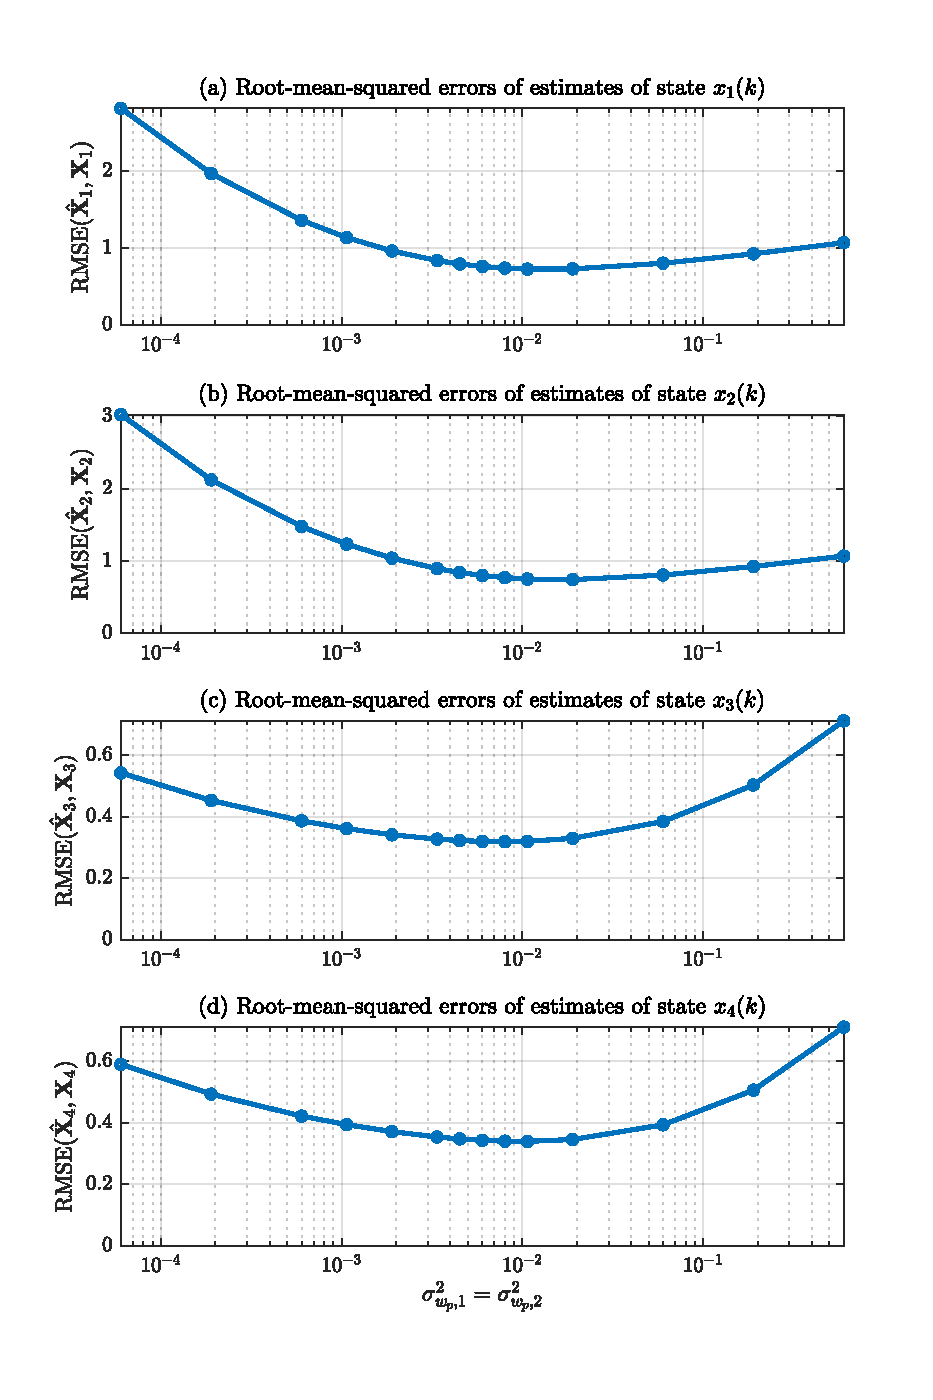
\includegraphics[width=14cm]{images/rod_obs_sim2_3KF_Q_seed_0.pdf}
	\caption{Tuning of Kalman filter KF3 – $2\times2$ system}
	\label{fig:sim-sys-2x2-KF3-tuning}
\end{figure}
	

\section{Sensitivity analyses}

\subsection{Pseudo-random numbers}

Many of the simulation results are sensitive to the initialization of the pseudo-random number generator (PRNG) used to simulate random processes. In particular, the RODD step disturbance (\ref{eq:wpk2}) is simulated by generating three pseudo-random sequences, two random noise sequences and a random binary sequence to simulate the infrequent shocks.  Since the random shocks are infrequent and tend to have a large magnitude, their effect on the simulation results can be significant.

To visualize this effect, consider the plot in Figure \ref{fig:rod-obs-sim-1-3KF-seed-crmse-statsplot}. This shows the RMSE of the output estimates of the three Kalman filters described in Section \ref{sim-obs-lin-1} for 10 simulations, each generated with a different \textit{seed}—the seed is a scalar argument used to initialize the PRNG algorithm in a unique state. The RMSE is calculated for every simulation duration, $t_N=0.5,1,1.5,...,2500$. The coloured areas represent the range between the lowest and the highest RMSE obtained for the 10 different simulations of each duration. The dark lines represent the median values.

\begin{figure}[htp]
	\centering
	\includegraphics[width=14cm]{images/rod_obs_sim1_3KF_seed_crmse_statsplot.pdf}
	\caption{Effect of random variables on the RMSE results.}
	\label{fig:rod-obs-sim-1-3KF-seed-crmse-statsplot}
\end{figure}

As expected, the differences in the results due to PRNG initialization are smaller the greater the length of the simulation. However, the magnitude of the differences is not the same for each observer. The RMSE values of KF1, which has the lowest gain, are more sensitive to the random initialization than the other two filters. Therefore it is not possible to estimate the expected value of the RMSE of KF1 from a single simulation of this duration---a longer simulation or a larger number of simulations would be needed. On the other hand, the variations in the RMSEs of KF2 and KF3 are significantly lower. After the full length of the simulations ($t_N=2500$), the RMSE of KF2 is between -0.0039 (-2.5\%) and 0.0019 (1.3\%) of the median value, which is $0.1550$.  That of KF3 is between -0.0035 (-4.0\%) / 0.0047 (5.3\%) of the median, 0.0889.  Therefore it is reasonable to conclude that the RMSE of KF3 is consistently about 0.05 lower than that of KF2. Note that the RMSEs of KF2 and KF3 reported in Section \ref{sim-obs-lin-1} are \alert{0.XXXX} and \alert{0.XXXX}. These values are both within the minimum and maximum values from this sensitivity analysis (in fact, the simulation output used to produce the main results is one of the 10 shown here).

A similar sensitivity analysis was carried out on the results of the Kalman Filter tuning shown in Figure \ref{eq:sim-sys-siso-KF3-Q}, where KF3 was tuned using a set of 5000 input-output samples from the system. Figure \ref{fig:sim-sys-siso-KF3-sensitivity} shows the variation in this result when ten different sets of pseudo-random simulation data are used.  Although there is considerable variation in the RMSE values for each parameter value, the best overall choice of $\sigma_{w_p}$ to achieve the lowest average error across all 10 simulations was found to be the same as that of the single simulation (0.01).

\begin{figure}[htp]
	\centering
	\includegraphics[width=14cm]{images/rod_obs_sim1_3KF_Q_statplot.pdf}
	\caption{Sensitivity of Kalman filter tuning – SISO system}
	\label{fig:sim-sys-siso-KF3-sensitivity}
\end{figure}

Figure \ref{fig:sim-sys-2x2-KF3-tuning-sens} shows the results of a similar sensitivity analysis on the results presented in Figure \ref{fig:sim-sys-2x2-KF3-tuning}.

\begin{figure}[htp]
	\centering
	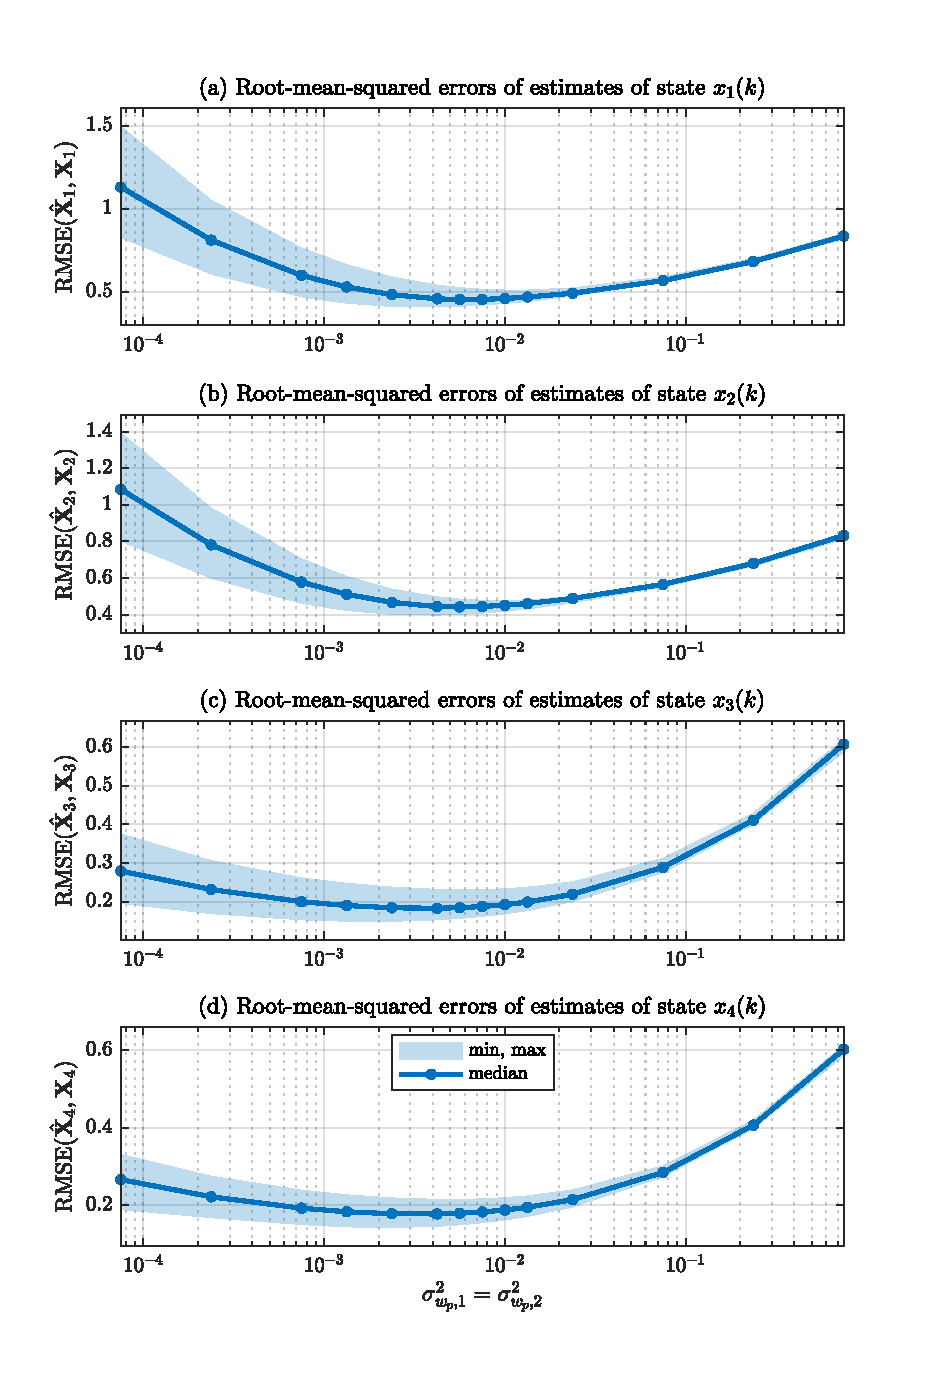
\includegraphics[width=14cm]{images/rod_obs_sim2_3KF_Q_statplot.pdf}
	\caption{Sensitivity of Kalman filter tuning – $2\times2$ system}
	\label{fig:sim-sys-2x2-KF3-tuning-sens}
\end{figure}

                % annexe A

%<!articles>\bibliography{}                 % production de la bibliographie
%<!articles>
\end{document}
%</gabarit>
%
% ^^A Gabarits des parties du document
%<*resume>
\chapter*{Résumé}               % ne pas numéroter
\label{chap-resume}             % étiquette pour renvois
\phantomsection\addcontentsline{toc}{chapter}{\nameref{chap-resume}} % inclure dans TdM

\begin{otherlanguage*}{french}
  <Texte du résumé en français. Obligatoire.>
\end{otherlanguage*}
%</resume>
%
%<*abstract>
\chapter*{Abstract}             % ne pas numéroter
\label{chap-abstract}           % étiquette pour renvois
\phantomsection\addcontentsline{toc}{chapter}{\nameref{chap-abstract}} % inclure dans TdM

\begin{otherlanguage*}{english}
  <Text of English abstract. Optional, but recommended.>
\end{otherlanguage*}
%</abstract>
%
%<*remerciements>
\chapter*{Remerciements}        % ne pas numéroter
\label{chap-remerciements}      % étiquette pour renvois
\phantomsection\addcontentsline{toc}{chapter}{\nameref{chap-remerciements}} % inclure dans TdM

<Texte des remerciements en prose.>
%</remerciements>
%
%<*avantpropos>
\chapter*{Avant-propos}         % ne pas numéroter
\label{chap-avantpropos}        % étiquette pour renvois
\phantomsection\addcontentsline{toc}{chapter}{\nameref{chap-avantpropos}} % inclure dans TdM

<Texte de l'avant-propos. Obligatoire dans une thèse ou un mémoire par
articles.>
%</avantpropos>
%
%<*introduction>
\chapter*{Introduction}         % ne pas numéroter
\label{chap-introduction}       % étiquette pour renvois
\phantomsection\addcontentsline{toc}{chapter}{\nameref{chap-introduction}} % inclure dans TdM

<Texte de l'introduction. La thèse ou le mémoire devrait normalement
débuter par une introduction. Celle-ci est traitée comme un chapitre
normal, sauf qu'elle n'est pas numérotée.>
%</introduction>
%
%<*chapitre>
\chapter{<Titre du chapitre ou de l'article>}     % numéroté
\label{chap-}                   % étiquette pour renvois (à compléter!)

%<articles>\section{Résumé}
%<articles>
%<articles>\begin{otherlanguage*}{french}
%<articles>  <Résumé de l'article en français. Obligatoire.>
%<articles>\end{otherlanguage*}
%<articles>
%<articles>\section{Abstract}
%<articles>
%<articles>\begin{otherlanguage*}{english}
%<articles>  <English abstract of the paper. Optional, but recommended.>
%<articles>\end{otherlanguage*}
%<articles>
<Texte du chapitre ou de l'article.>
%<articles>
%<articles>\bibliographystyle{}              % style de la bibliographie
%<articles>\bibliography{}                   % production de la bibliographie
%</chapitre>
%
%<*conclusion>
\chapter*{Conclusion}           % ne pas numéroter
\label{chap-conclusion}         % étiquette pour renvois
\phantomsection\addcontentsline{toc}{chapter}{\nameref{chap-conclusion}} % inclure dans TdM

<Texte de la conclusion. Une thèse ou un mémoire devrait normalement
se terminer par une conclusion placée avant les annexes, le cas
échéant. La conclusion est traitée comme un chapitre normal, sauf
qu'elle n'est pas numérotée.>
%</conclusion>
%
%<*annexe>
\chapter{<Titre de l'annexe>}     % numérotée
\label{chap-}                   % étiquette pour renvois (à compléter!)

<Texte de l'annexe.>
%</annexe>
% \fi
